\documentclass{inputs/mc2015}
%
%=================================================================================================
% new commands
% +++++++++++++++++++++++++++++++++++++++++++++++++++++++++++++++++++++++++++++++++++++++++++++++++
\newcommand{\nc}{\newcommand}

\renewcommand{\div}{\mbold{\nabla}\! \cdot \!}
\newcommand{\grad}{\mbold{\nabla}}
\newcommand{\divv}[1]{\boldsymbol{\nabla}^{#1}\! \cdot \!}
\newcommand{\gradd}[1]{\mbold{\nabla}^{#1}}
\newcommand{\mbold}[1]{\boldsymbol#1}
% latex shortcuts
\newcommand{\bea}{\begin{eqnarray}}
\newcommand{\eea}{\end{eqnarray}}
\newcommand{\be}{\begin{equation}}
\newcommand{\ee}{\end{equation}}
\newcommand{\bal}{\begin{align}}
\newcommand{\eali}{\end{align}}
\newcommand{\bi}{\begin{itemize}}
\newcommand{\ei}{\end{itemize}}
\newcommand{\ben}{\begin{enumerate}}
\newcommand{\een}{\end{enumerate}}
\usepackage{amsthm}
\newtheorem*{remark}{Remark}
% DGFEM commands
\newcommand{\jmp}[1]{[\![#1]\!]}                     % jump
\newcommand{\mvl}[1]{\{\!\!\{#1\}\!\!\}}             % mean value
\newcommand{\keff}{\ensuremath{k_{\textit{eff}}}\xspace}
% shortcut for domain notation
\newcommand{\D}{\mathcal{D}}
% vector shortcuts
\newcommand{\vo}{\mbold{\Omega}}
\newcommand{\vr}{\mbold{r}}
\newcommand{\vn}{\mbold{n}}
\newcommand{\vnk}{\mbold{\mathbf{n}}}
\newcommand{\vj}{\mbold{J}}
\newcommand{\eig}[1]{\| #1 \|_2}
%
\newcommand{\EI}{\mathcal{E}_h^i}
\newcommand{\ED}{\mathcal{E}_h^{\partial \D^d}}
\newcommand{\EN}{\mathcal{E}_h^{\partial \D^n}}
\newcommand{\ER}{\mathcal{E}_h^{\partial \D^r}}
\newcommand{\reg}{\textit{reg}}
%
\newcommand{\norm}{\textrm{norm}}
\renewcommand{\Re}{\textrm{Re}}
\newcommand{\Pe}{\textrm{P\'e}}
\renewcommand{\Pr}{\textrm{Pr}}
%
\newcommand{\resi}{R}
%\newcommand{\resinew}{\tilde{D}_e}
\newcommand{\resinew}{\widetilde{\resi}}
\newcommand{\resisource}{\widetilde{\resi}^{source}}
\newcommand{\matder}[1]{\frac{\textrm{D} #1}{\textrm{D} t}}
%
\newcommand{\Gammakj}{\Gamma_{k \to j}}

% extra space
\newcommand{\qq}{\quad\quad}
% common reference commands
\newcommand{\eqt}[1]{Eq.~(\ref{#1})}                     % equation
\newcommand{\eqts}[1]{Eqs.~(\ref{#1})}                     % equations
\newcommand{\fig}[1]{Fig.~\ref{#1}}                      % figure
\newcommand{\tbl}[1]{Table~\ref{#1}}                     % table
\newcommand{\sct}[1]{Section~\ref{#1}}                   % section
\newcommand{\app}[1]{Appendix~\ref{#1}}                   % appendix
\newcommand{\lem}[1]{Lemma~\ref{#1}}                   % lemma
\newcommand{\theo}[1]{Theorem~\ref{#1}}                   % theorem
%
\newcommand{\ie}{i.e.,\@\xspace}
\newcommand{\eg}{e.g.,\@\xspace}
\newcommand{\psc}[1]{{\sc {#1}}}
\newcommand{\rs}{\psc{R7}\xspace}
%
\newcommand\br{\mathbf{r}}
%\newcommand{\tf}{\varphi}
\newcommand{\tf}{b}
%
%\renewcommand{\dim}{\ensuremath{\texttt{dim}}\xspace}
%
\newcommand{\tcr}[1]{\textcolor{red}{#1}}
\newcommand{\tcb}[1]{\textcolor{blue}{#1}}
  \newcommand{\tcg}[1]{\textcolor{green}{#1}}
\newcommand{\mt}[1]{\marginpar{ {\tiny #1}}}

\newtheorem{theorem}{Theorem}[section]
\newtheorem{lemma}[theorem]{Lemma}

%%%%%%%%%%%%%%%%%%%%%%%%%%%%%%%%%%%%%%%%%%%%%%%%%%%%%%%%%%%%%%%%%%%%%
\usepackage[T1]{fontenc}         % Use T1 encoding instead of OT1
\usepackage[utf8]{inputenc}      % Use UTF8 input encoding
\usepackage{microtype}           % Improve typography
\usepackage{booktabs}            % Publication quality tables
\usepackage{amsmath}
\usepackage{amssymb}
\usepackage{mathrsfs}
% more math
\usepackage{amsfonts}
\usepackage{amstext}
\usepackage{amsbsy}
\usepackage{mathbbol} 
\usepackage{graphicx}
\usepackage{float}
\usepackage[exponent-product=\cdot]{siunitx}
\usepackage[colorlinks,breaklinks]{hyperref}
\hypersetup{linkcolor=black, citecolor=black, urlcolor=black}
\usepackage{lineno}
\linenumbers

\usepackage{lipsum}


\usepackage{color}
\usepackage{caption}
\usepackage{subcaption}
\usepackage{mathrsfs}
% more math
\usepackage{amsfonts}
\usepackage{amstext}
\usepackage{amsbsy}
\usepackage{mathbbol} 


\def\equationautorefname{Eq.}
\def\figureautorefname{Fig.}

%%%%%%%%%%%%%%%%%%%%%%%%%%%%%%%%%%%%%%%%%%%%%%%%%%%%%%%%%%%%%%%%%%%%%
% Insert authors' names and short version of title in lines below

\authorHead{Marc O. Delchini, Jean C. Ragusa, Ray A. Berry}
\shortTitle{Pressure wave simulations with RELAP-7}

%%%%%%%%%%%%%%%%%%%%%%%%%%%%%%%%%%%%%%%%%%%%%%%%%%%%%%%%%%%%%%%%%%%%%
\begin{document}

%\title{Application of the reactor system code RELAP-7 to single- and two-phase flow water-hammer problems}
\title{Simulations of single and two-phase pressure waves with the RELAP-7 system code}

\author{Marc O. Delchini}
\affil{
  Reactor and Nuclear Systems Division\\
  Oak Ridge National Laboratory\\
  Oak Ridge, TN, 37831\\
  delchinimg@ornl.gov}
\author{Jean C. Ragusa}
\affil{
  Department of Nuclear Engineering\\
  Texas A\&M University\\
  College Station, TX 77843\\
  jean.ragusa@tamu.edu}

\author{Ray A. Berry}
%\author{David Andrs}
%\author{Richard Martineau}
\affil{
  Idaho National Laboratory\\
	Idaho Falls, ID 83415\\
  ray.berry@inl.gov
}

\maketitle

\begin{abstract}

%Evaluation of pressure waves has been a field of interest for many years in nuclear reactors and currently relies on a variety of computer codes such as RELAP-5 (REF), TRACE to name a few. 
Propagation of pressure waves in single and two-phase flows is of key interest for nuclear safety analyses, reactor design, construction and life extension of nuclear reactors. In this work, we assess the capabilities of RELAP-7, the next-generation nuclear reactor system code, to solve single- and two-phase flows developing pressure waves. RELAP-7 is based on a 7-equation, two-phase flow model, with distinct phasic pressures. It is well established that these hyperbolic conservation laws can develop shocks and discontinuities and thus, require a stabilization 
numerical method. The all-Mach flow Entropy Viscosity Method (EVM) is now employed in RELAP-7 as a viscous stabilization approach. 
%The entropy viscosity technique is a viscous regularization technique: adequate dissipation terms (viscous fluxes) are 
%added to the governing laws while ensuring the entropy minimum principle still holds. Viscosity coefficients modulate the magnitude of the 
%added dissipations such that they are large in shock regions and vanishingly small elsewhere. 
In this paper, we briefly describe the implementation of the EVM and use open-literature test cases that exhibit pressure waves to show that the entropy viscosity method performs adequately for these single- and two-phase cases. \\
%Method are demonstrated in the system code RELAP-7 by simulating pressure-wave propagation phenomena with single- and two-phase flow conditions taken from the published litereature. 
%
\emph{Key Words}:  RELAP-7 ; seven-equation model; entropy viscosity method ; low-Mach flow ; pressure waves ; single phase flows ; two-phase flows.
\end{abstract}

%%%%%%%%%%%%%%%%%%%%%%%%%%%%%%%%%%%%%%%%%%%%%%%%%%%%%%%%%%%%%%%%%%%%%%%%%%%%%
\section{Introduction}\label{sec:intro}
%%%%%%%%%%%%%%%%%%%%%%%%%%%%%%%%%%%%%%%%%%%%%%%%%%%%%%%%%%%%%%%%%%%%%%%%%%%%%
%
%\begin{itemize}
%\item objective: test Relap-7 with pressure-waves phenomena.
%\item list of situations encountered in nuclear reactors that involve pressure wave phenomena (see Soloko. for details).
%\item bibliography: includes papers that deal with water-hammer tests and also with pressure-wave phenomena.
%\item 
%\end{itemize}
%
The proper simulation of pressure waves in nuclear reactors has been a field of interest for many years. Currently, nuclear reactor safety relies on a variety of system-level computer codes such as RELAP-5 \cite{relap5}, TRACE \cite{trace} and WAHA \cite{waha-manual}, to name a few. Pressure waves, or pressure shocks, can occur in single- and two-phase flows and are important in the design and safety assessment of nuclear reactors. Several examples of destructive pressure wave propagation in nuclear reactor coolant systems are described in \cite{watkins-berry-1979}. Most of them result from variations of the following three scenarios, (i) check valve closures, (ii) slug flow in a voided line and (iii) steam bubble collapse. For instance, the rapid, intentional or accidental, closing of a turbine valve causes pressure waves that can lead to cavitation and pipe failure if the pressure variations exceed the manufacturer's specifications. Other pressure waves are caused by the rupture of a pressurized pipe or loss-of-coolant accident (LOCA): an expansion wave propagates in the pipe towards the reactor core system which could threaten the integrity of the reactor. A possible path towards validating a computer code for the simulation of pressure waves could be (i) to run shock tube tests that are commonly used in the literature to assess the robustness and the accuracy of a numerical method, and (ii) to validate the physical models by running benchmark tests such as waterhammer tests. In the past decades, several studies have been performed to assess the capabilities of system codes to calculate the propagation of pressure waves in piping systems. Studies on pressure wave propagation have showed that the system code RELAP-5 can achieve sufficient accuracy when using sufficiently small time steps and grid size, even though the code was not initially designed for such purpose \cite{tiselji-gale}. Waterhammer benchmark tests have also been simulated with the system codes RELAP-5 \cite{Serre-bestion, bestion-serre-2012, Sokolowski-Koszela} and CATHARE \cite{cathare} and have shown a good agreement with experimental data. More recently, the computer code WAHA was used to simulate waterhammer experiments \cite{waha} and the experiment by Takeda and Toda \cite{costa-tiselji}. 
%Computer codes are commonly used to study pressure wave propagation in nuclear hydraulic systems and validated against benchmarks (Edward's pipe (REF), single- and two-phase flow water-hammer benchmark).

The objective of this work is to assess the current capabilities of the RELAP-7 system code (Reactor Excursion and Leak Analysis Program) \cite{Berry_Peterson_2014} to solve rapid pressure waves that can occur in nuclear reactors during transients and accident scenarios. RELAP-7 is the next-generation nuclear reactor system analysis code under development at the Idaho National Laboratory (INL) and is based on the modern scientific framework  MOOSE \cite{MOOSE} (Multi-Physics Object Oriented Simulation Environment) that is itself built upon the PETSc and LibMesh libraires, among others.
%The RELAP-7 code \cite{Berry_Peterson_2014} is built using modern scientific software libraries (the Multi-Physics Object Oriented Simulation Environment MOOSE \cite{MOOSE}, 
%itself built upon PETSc and LibMesh, among others).  
%
%\tcb{Equations in RELAP-7 and numerical methods} \\ 
The primary basis for RELAP-7's governing theory includes the single-phase Euler equations \cite{Toro} and the 7-equation two-phase flow model of \cite{SEM, Berry_MC_2014}. It is well established that hyperbolic conservation laws can develop shocks and discontinuities \cite{Leveque} and, therefore, require stabilization of the discretized equations. For the single-phase Euler equations, numerous numerical methods are available in the literature both for discontinuous and continuous discretization schemes
\cite{Toro, Lapidus_paper, LMP, Lapidus_book, Roe, SUPG}. Until recently and to the best of our knowledge, the 7-equation model was primarily spatially discretized using discontinuous schemes with approximate 
Riemann solvers derived using well-established approaches for single-phase flows, while using an upwind-type flux for the non-conservative terms 
\cite{Saurel_2001a, Saurel_2001b, Li_2004, Zein_2010, Ambroso_2012}. Such an approach is made possible thanks to the hyperbolic nature of the 7-equation model. As opposed to two-phase flow models assuming pressure-equilibrium between phases that are ill-posed in a Cauchy sense \cite{stewart-wendroff-1984}, the seven-equation model has seven unconditionally real eigenvalues and a set of right eigenvectors that are independent in some limits \cite{coquel_herard}. Characteristics can also be derived and used to implement boundary conditions. Another advantage of the seven-equation model over the more traditional two-phase flow models used in nuclear engineering, is the presence of the volume fraction equation that should allow better accuracy when simulating waterhammers. Additionally, the seven-equation model can successively devolves to the six-equation model, the five-equation model of Kapila \cite{Kapila_2001} and the homogeneous equilibrium model (HEM) by successively relaxing the phasic pressures, velocities and temperatures. From a numerical prospective, however, the seven-equation model remains challenging because of the large number of equations to solve and the presence of non-conservative terms.
In RELAP-7, the conservation laws, i.e., the single- and two-phase conservation laws, are discretized using a \emph{continuous Galerkin finite element method} and the resulting discrete equations are stabilized using a recently developed artificial viscosity called the Entropy Viscosity Method (EVM) \cite{jlg1, jlg2}.
%One of the identified advantage of the seven-equation two-phase flow model over the six-equation model is its well-possesses that allows the use of high-order numerical method for better accuracy.
%and implements the single phase Euler equations and the Seven-equation two-phase flow model that are both well-posed conservation laws. The all-Mach flow Entropy Viscosity Method is now implemented and employed in RELAP-7 as a stabilization numerical method for both above models and allow to solve for flows developing pressure waves while ensuring high-order accuracy for smooth flows.
%
%Single- and two-phase flow pressure wave problems are simulated using RELAP-7 (Reactor Excursion and Leak Analysis Program) \cite{Berry_Peterson_2014},. 
%
%Water hammer, or hydraulic shock, is a pressure surge or wave caused when a fluid in motion is forced to stop or change direction abruptly. 
%In nuclear power plants, water hammers commonly occur 
%in case of an inflow of sub-cooled water into pipes or other parts of the equipment, which are filled with steam or steam-water mixture; they also
%happen as the consequence of valve closing or opening actions or of breaks in pipes, with single phase or two-phase flow. 
% when a valve closes suddenly at an end of a pipe system, and a pressure wave propagates in the pipe. 

%The RELAP-7 code \cite{Berry_Peterson_2014} is built using modern scientific software libraries (the Multi-Physics Object Oriented Simulation Environment MOOSE \cite{MOOSE}, 
%itself built upon PETSc and LibMesh, among others).  
%%
%The primary basis for RELAP-7's governing theory includes single-phase Euler equations \cite{Toro} and the 7-equation two-phase flow model of \cite{SEM, Berry_MC_2014}. 
%This two-phase flow model is strictly hyperbolic, as opposed to the 6-equation model RELAP-5.  
%It is well established that hyperbolic conservation laws can develop shocks and discontinuities \cite{Leveque} and, thecoquel_herardore, require stabilization 
%of the discretized equations. For single-phase Euler equations, numerous numerical methods are available both for discontinuous and continuous discretization schemes 
%\cite{Toro, Lapidus_paper, LMP, Lapidus_book, Roe, SUPG}. Until recently, the 7-equation model was primarily discretized in space using discontinuous schemes with approximate 
%Riemann solvers derived using well-established approaches for single-phase flows, while using an upwind-type flux for the non-conservative terms 
%\cite{Saurel_2001a, Saurel_2001b, Li_2004, Zein_2010, Ambroso_2012}. 
%%
%In RELAP-7, the conservation laws are discretized using a \emph{continuous Galerkin finite element method} and the resulting discrete equations are stabilized using 
%the Entropy Viscosity Method \cite{jlg1, jlg2}.
%  that is independent of the type of spatial discretization (finite volume, continuous or discontinuous finite elements, ...) and thus may be applied ubiquitously.
 The EVM is a viscous regularization technique wherein adequate dissipation terms (viscous fluxes) are added to the governing laws while ensuring 
that the minimum entropy principle holds. Viscosity coefficients modulate the magnitude of the added dissipations such that they are large in shock regions and vanishingly 
small elsewhere. The entropy viscosity coefficients are taken proportional to the entropy production while, at the same time, being bounded from above by a first-order 
viscosity coefficient that reduces the spatial discretization to be similar to a first-order Godunov scheme (the latter being known to be overly dissipative but monotone 
\cite{Toro}). Hence, entropy production in shocks will result in large viscosity coefficients and thus will avoid spurious oscillations. In order to solve for 
low-Mach flows \cite{LowMach1, LowMach2, LowMach3}, the original version of the EVM was modified and new definitions of the viscosity coefficients 
were proposed to ensure well-scaled dissipative terms in the low-Mach asymptotic limit while preserving the capabilities of the method to resolve shocks and discontinuities 
\cite{Marco_dissertation, Marco_paper_low_mach}. The same approach was used to extend the method to the 7-equation two-phase flow model 
\cite{Marco_paper_7_equ, Marco_dissertation}. 

The remaining of this paper is organized as follows. In \sct{sct:model}, the single- and two-phase flow models, regularized with the EVM, are recalled along with the all-Mach flow definitions of the viscosity coefficients. 
%After providing the spatial and temporal discretization method in \sct{sec:disc}, 
After briefly detailing the spatial and temporal discretization methods, numerical results of flows developing pressure waves taken from the published literature and obtained with the system code RELAP-7 are presented in \sct{sec:results}. A set of shock tube tests \cite{Sokolowski-Koszela} are run to assess the robustness and the accuracy of the EVM when using the stiffened/ideal gas equation of state and steam-water tables.
%Water hammer-like tests are also investigated \cite{Serre-bestion}.
%
%Tests include a set of single- and two-phase flow shock tubes \cite{Sokolowski-Koszela} that are commonly used in the literature to assess the robustness and accuracy of a numerical method. Then, and water-hammer test-like \cite{Serre-bestion}.
%We focused on single- and two-phase flow shock tubes taken from the published literature \cite{Sokolowski-Koszela, Serre-bestion} and also 
%tests taken from the published literature \cite{Sokolowski-Koszela, Serre-bestion} and developing pressure waves are presentedRELAP-7 is assessed against single and two-phase flow problems developing pressure waves and water-hammer like tests taken from the published literature .

%
%%%%%%%%%%%%%%%%%%%%%%%%%%%%%%%%%%%%%%%%%%%%%%%%%%%%%%%%%%%%%%%%%%%%%%%%%%%%%
%%%%%%%%%%%%%%%%%%%%%%%%%%%%%%%%%%%%%%%%%%%%%%%%%%%%%%%%%%%%%%%%%%%%%%%%%%%%%
\section{Single phase and two-phase flow models}\label{sct:model}
%%%%%%%%%%%%%%%%%%%%%%%%%%%%%%%%%%%%%%%%%%%%%%%%%%%%%%%%%%%%%%%%%%%%%%%%%%%%%
%%%%%%%%%%%%%%%%%%%%%%%%%%%%%%%%%%%%%%%%%%%%%%%%%%%%%%%%%%%%%%%%%%%%%%%%%%%%%
%
In this section, the single- and the two-phase flow models implemented in RELAP-7 are recalled, along with their viscous regularization via the EVM
and the definition of the viscosity coefficients that are appropriate for all-Mach flows. % definition of used in the application of the numerical method called the Method (EVM). 
%
%------------------------------------------------------------------------------------------------------------------
\subsection{1-D Euler equations with viscous regularization}\label{sec:single-model}
%------------------------------------------------------------------------------------------------------------------
The conservative form of the 1-D Euler equations \cite{Toro} is implemented in RELAP-7 \cite{Berry_Peterson_2014} and used to simulate single-phase flows in light water reactors. An equation of state ($eos$) that depends upon the the specific volume $v = \rho^{-1}$ and 
specific internal energy $e$ serves as a closure relation to compute the pressure, $P = eos(v, e)$. Stabilization of the scheme is ensured by the Entropy Viscosity Method (EVM), with its extension to be an all-Mach flow numerical method \cite{Marco_paper_low_mach, Marco_dissertation}. The 1-D Euler equations with the viscous regularization and the definition of the viscosity coefficients used in the application of the EVM and implemented in RELAP-7 are recalled in \eqt{eq:euler-eq} through (\ref{eq:single-visc-def}). The viscous regularization terms are denoted by the dissipative flux $\mbold D$ on the right-hand side.
%
\begin{subequations}\label{eq:euler-eq}
\begin{equation}
\partial_t \mbold U + \partial_x \mbold F \left( \mbold U \right) = \partial_x \mbold D \left( \mbold U \right) \, ,
\end{equation}
\text{where}
\begin{equation}
\mbold U = \left[ 
\begin{array}{l}
\rho \\
\rho u \\
\rho E  \\
\end{array}
\right], \,
%
\mbold F \left( \mbold U \right) = \left[ 
\begin{array}{l}
\rho u \\
\rho u^2 + P \\
u \left( \rho E + P \right)  \\
\end{array}
\right]
\end{equation}
\text{and}
\begin{equation}
\mbold D \left( \mbold U \right) = \left[ 
\begin{array}{l}
 f \\
 g + uf \\
 h + ug - 0.5 u^2 f \\
\end{array}
\right]\, , 
\end{equation}
\end{subequations}
%
where $E$ and $u$ are the specific total energy and the velocity of the fluid, respectively. The partial derivatives with respect to time and space are denoted by $\partial_t$ and $\partial_x$. The expressions for the dissipative terms, $f$, $g$, and $h$, were obtained by deriving the entropy residual and applying the minimum entropy principle \cite{jlg}:
%
\begin{equation}
f = \kappa \partial_x \rho , \ g = \mu \rho \partial_x u, \text{  and  } h = \kappa \partial_x \left( \rho e \right) \, . 
\end{equation}
%
Definitions of the viscosity coefficients $\mu$ and $\kappa$, given later in \eqt{eq:single-visc-def}, are derived in \cite{Marco_paper_low_mach} using a non-dimensionalization of Euler equations in order to retrieve well-scaled dissipative terms for any Mach number (so that adequate stabilization is provided in supersonic, transonic and low-Mach flows). Each viscosity coefficient is computed from an upper bound denoted by the subscript $max$, and an entropy viscosity coefficient denoted by the subscript $e$. The upper-bound viscosity coefficient is defined proportional to the maximum eigenvalue of the hyperbolic system and is designed to be over-dissipative and similar to a first-order Godunov scheme (\eqt{eq:visc-def-max}). The entropy viscosity coefficient is set proportional to the entropy residual, $R_e(x,t)$.
%, and a jump denoted by $J$. 
The entropy residual is known to be peaked in the shock region \cite{Leveque} and thus can be used to detect and track shocks. As proposed in \cite{Marco_paper_low_mach} and recalled in \eqt{eq:ent-res}, the entropy residual is computed locally using pressure, density, sound speed, $c$, as follows:
%
\begin{equation}\label{eq:ent-res}
R_e(x,t) = \frac{DP}{Dt} - c^2\frac{D\rho}{Dt} \, ,
\end{equation}
%
where $\frac{D (\cdot)}{Dt} := \partial_t(\cdot) + u  \partial_x(\cdot)$ is the material derivative. 
%The jump $J$ is function of the the jump of pressure and density gradients across the face shared by two cells of the mesh and its definition is given in \eqt{eq:jump}:
%%
%\begin{equation}\label{eq:jump}
%J = \max \left( |u| [[ \partial_x P ]], \, |u| (Mc)^2 [[ \partial_x \rho ]] \right) \, .
%\end{equation}
%%
%$[[ x ]]$ denotes the jump of the quantity $x$ across a face and $M = |u| / c$ is the Mach number. 
The all-Mach flow definition of the viscosity coefficients $\mu$ and $\kappa$ proposed in \cite{Marco_paper_low_mach} is now recalled:
%
\begin{subequations}\label{eq:single-visc-def}
\begin{align}\label{eq:single-visc-def-mu}
\mu(x,t) = \min \left( \mu_{max}(x,t), \, \mu_e(x,t) \right) \ \ \text{ and } \ \ \kappa(x,t) = \min \left( \kappa_{max}(x,t), \, \kappa_e(x,t) \right)
\end{align}
\text{where}
\begin{align}\label{eq:visc-def-max}
\mu_{max}(x,t) = \kappa_{max}(x,t) = \tfrac{1}{2} \Delta x \left( |u| + c \right)\, ,
\end{align}
\begin{align}\label{eq:visc-def-ent}
%\mu_e(x,t) = \frac{h^2}{\norm_\mu} \max \left( R_e(x,t), J \right)\, ,
\mu_e(x,t) = \frac{\Delta x^2 R_e(x,t)}{\norm_\mu}\, , \quad 
%\kappa_e(x,t) = \frac{h^2}{\norm_\kappa} \max \left( R_e(x,t), J \right)
\kappa_e(x,t) = \frac{\Delta x^2 R_e(x,t)}{\norm_\kappa} 
\end{align}
\text{with}
\begin{equation}
\norm_\kappa = \norm_\mu = \rho \left( \max ( \bar{|u|}, u ) \right)^2\, 
\end{equation}
%\text{and}
%\begin{equation}
%\norm_\kappa = \norm_\mu
%\end{equation}
\end{subequations}
%
%\tcb{replace h with $\Delta x$} \\ 
where $\Delta x$ is the grid size. The normalization parameters, $\norm_\mu$ and $\norm_\kappa$, appearing in the definition of the entropy viscosity coefficient $\mu_e$ and $\kappa_e$, respectively, are function of the average velocity over the computational domain $\bar{|u|}$, the local velocity, u, and the local density $\rho$. This definition was chosen to ensure the correct scaling of the viscosity coefficients in the vicinity of the shock as detailed in \cite{Marco_paper_low_mach}, and also to avoid dividing by zero when the fluid is at locally at rest. Note that other normalization functions were proposed
%the Mach number $M$ through the functions $a(M)$. In this paper, $a(M)$ is set to $\max( |\bar{u}|,  )$ 
in Eq.~(28) of \cite{Marco_paper_low_mach}. 
%an expression for $a(M)$ is proposed and used for both functions in this paper as well. 
%\tcr{is this correct? I think we are mostly using the shock function, the low-mach paper spends more time describing the Mach function, which is not used much here, right?} \tcb{You are right, done}
%
%------------------------------------------------------------------------------------------------------------------
\subsection{1-D Seven-Equation two-phase flow model with viscous regularization}\label{sec:two-phase-model}
%------------------------------------------------------------------------------------------------------------------
%
RELAP-7 \cite{Berry_Peterson_2014} uses the seven-equation two-phase flow model \cite{SEM} to simulate the behavior of two-phase flows in light water reactors. In this model, each phase is treated as being compressible, exhibits independent thermodynamical and mechanical properties, and is described by its own equation of state, $P_k = eos_k(\rho_k,e_k)$, $k$ being the phase index. This system of equations is hyperbolic and has seven real eigenvalues. The 1-D 7-equation model is recalled in \eqt{eq:sem-eq} for a liquid phase in interaction with a gas phase denoted by the subscript $liq$ and $gas$, respectively. Equations for the vapor phase can be devised from \eqt{eq:sem-eq} by simply substituting the subscripts $_{liq}$ to $_{gas}$ and $_{gas}$ to $_{liq}$.
%
%
\begin{subequations}\label{eq:sem-eq}
\begin{equation}
\partial_t \mbold U_{liq} + \partial_x \mbold F \left( \mbold U_{liq} \right) = \mbold N \left( \mbold U_{liq}, \, \mbold U_{gas} \right) + \mbold R \left( \mbold U_{liq}, \, \mbold U_{gas} \right) +  \partial_x \mbold D \left( \mbold U_{liq} \right) + \mbold S \left( \mbold U_{liq}, \, \mbold U_{gas} \right)\, ,
\end{equation}
\text{where}
%
\begin{equation}
\mbold U_{liq} = \left[ 
\begin{array}{l}
 \alpha_{liq} \\
( \alpha \rho )_{liq} \\
( \alpha \rho u )_{liq} \\
( \alpha \rho E )_{liq}  \\
\end{array}
\right], \,
%
\mbold F \left( \mbold U_{liq} \right) = \left[ 
\begin{array}{l}
 0 \\
( \alpha \rho u )_{liq} \\
( \alpha \rho u^2 + \alpha P )_{liq} \\
( \alpha u )_{liq} \left( \rho E + P \right)_{liq}  \\
\end{array}
\right], \,
\end{equation}
%
\begin{equation}
\mbold N \left( \mbold U_{liq}, \, \mbold U_{gas} \right) = \left[ 
\begin{array}{l}
 - u_{int} \partial_x \alpha_{liq} \\
 0 \\
P_{int} \partial_x \alpha_{liq} \\
P_{int} u_{int} \partial_x \alpha_{liq}  \\
\end{array}
\right], \,
\end{equation}
%
\begin{equation}
\mbold R \left( \mbold U_{liq}, \, \mbold U_{gas} \right) = \left[ 
\begin{array}{l}
 \mu_P \left( P_{gas} - P_{liq} \right)\\
0 \\
 \mu_P \left( P_{gas} - P_{liq} \right)\\
 \mu_P \bar{u}_{int} \left( P_{gas} - P_{liq} \right) + \lambda_u \bar{P}_{int} \left( u_{liq} - u_{gas} \right) - A_{int} h_{conv,liq} (T_{liq} - T_{int})\\
\end{array}
\right], \,
\end{equation}
%
\begin{equation}
\mbold S \left( \mbold U_{liq}, \, \mbold U_{gas} \right) = \left[ 
\begin{array}{l}
\Gamma A_{int} / \rho_{int} \\
 \Gamma A_{int} \\
\Gamma A_{int} u_{int} \\
\Gamma A_{int} E_{int} \\
\end{array}
\right] \, ,
\end{equation}
%
\text{and}
\begin{equation}\label{eq:diss-terms}
\mbold D\left( \mbold U_{liq} \right) = \left[ 
\begin{array}{l}
 l_{liq} \\
 ( f + \rho l )_{liq} \\
 ( g + uf + \rho u l)_{liq} \\
 ( h + ug + 0.5 u^2 f + \rho E l)_{liq} \\
\end{array}
\right] \, .
\end{equation}
\end{subequations}
%
The liquid volume fraction is denoted by  $\alpha_{liq}$ and the vapor volume fraction is computed from the algebraic relation $\alpha_{gas} = 1 - \alpha_{liq}$. The mass transfer between the liquid and vapor phases, $\Gamma$, the interfacial density, $\rho_{int}$ and the total energy $E_{int}$ are defined in Section 3.2.3 of \cite{Berry_Peterson_2014}. Following \cite{SEM}, the pressure ($P_{int}$) and velocity ($u_{int}$) interfacial variables, their respective average value $\bar{P}_{int}$ and $\bar{u}_{int}$, and the relaxation coefficients, $\mu_P$ and $\lambda_u$, are functions of the liquid and vapor acoustic impedances denoted by $Z_k = \rho_k c_k$ with $k = \{ liq, \ vap \}$, and computed with the following expressions:
%
\begin{subequations}
\label{eq:int_variables_def}
\begin{align}
  \label{E-R:83}
  P_{int} &= \bar{P}_{int} + \frac{Z_{liq}Z_{gas}}{Z_{liq}+Z_{gas}} sgn \left( \partial_x \alpha_{liq} \right) \cdot (u_{gas}-u_{liq}) \,,
  \\
  \bar{P}_{int} &= \frac{Z_{gas} P_{liq}+Z_{liq}P_{gas}}{Z_{liq}+Z_{gas}} \,,
 \\
  \label{E-R:84}
  u_{int} &= \bar{u}_{int} +  sgn \left( \partial_x \alpha_{liq}\right) \frac{P_{gas}-P_{liq}}{Z_{liq}+Z_{gas}} \,,
  \\
  \bar{u}_{int} &= \frac{Z_{liq} u_{liq}+Z_{gas} u_{gas}}{Z_{liq}+Z_{gas}} \, ,
  \\
  \mu_P &= \frac{A_{int}}{Z_{liq}+Z_{gas}} \, 
  \text{and }
  \lambda_u = \frac{1}{2} \mu_P Z_{liq} Z_{gas} \, ,
\end{align}
\end{subequations}
%
where the function $sgn(x)$ returns the sign of the variable $x$ and $A_{int}$ is the specific interfacial area that can be computed from a correlation; see, for instance, \cite{SEM}. The phasic heat transfer $h_{conv,k}$ is computed from a flow regime map that is detailed in Section 6.3 of \cite{Berry_Peterson_2014}. The interfacial temperature $T_{int}$ is defined as the saturation temperature for the interfacial pressure $P_{int}$. All other variables were previously defined and interphase mass transfer has been neglected. As for the single-phase Euler equations (\sct{sec:single-model}), the dissipative terms given in the vector $\mbold D\left( \mbold U_{liq} \right)$ have been derived from the minimum entropy principle and have the following definitions:
%
\begin{subequations}
\begin{equation}
l_{liq} = \beta_{liq} \partial_x \alpha_{liq} , \, f_{liq}= ( \alpha \kappa )_{liq} \partial_x \rho_{liq} , 
\end{equation}
\begin{equation}
 g_{liq} = ( \alpha \mu \rho )_{liq} \partial_x u_{liq} \, \text{ and } h_{liq} = ( \alpha \kappa )_{liq} \partial_x \left( \rho e \right)_{liq} \, . 
\end{equation}
\end{subequations}
%
The positive viscosity coefficients for the liquid phase $\beta_{liq}$, $\mu_{liq}$ an $\kappa_{liq}$ are defined by investigating the non-dimensionalized 7-equation two-phase flow model and performing a low-Mach asymptotic limit \cite{Marco_paper_7_equ}. The viscosity coefficients $\mu_{liq}$ and $\kappa_{liq}$ are found identical to the one given in \eqt{eq:single-visc-def} for the single-phase Euler equation (this is expected since the 7-equation model degenerates to Euler equations when one phase disappears). The approach employed to define the viscosity coefficient $\beta_{liq}$ is similar to the logic followed for hyperbolic scalar equations \cite{jlg1, jlg2}: an entropy equation can be derived from the volume fraction equation and used in the definition of the viscosity coefficient $\beta_{liq}$ . Following the work by Guermond et al. \cite{jlg1, jlg2}, one obtains:
%
\begin{subequations}
\begin{equation}
\beta_{liq}(x,t) = \min \left( \beta_{max, liq}(x,t), \, \beta_{e, liq}(x,t) \right)
\end{equation}
%
\text{with}
%
\begin{equation}
\beta_{max, liq}(x,t) = \tfrac{1}{2} \Delta x | u_{int}(x,t) |
\end{equation}
%
\text{and}
%
\begin{equation}
%\beta_{e,liq}(x,t) =  h^2 \frac{\max \left( | R_{\alpha,liq}(x,t) |, J_{\alpha_{liq}} \right)}{|| \alpha_{liq} - \bar{\alpha}_{liq}||_\infty},
\beta_{e,liq}(x,t) =  \frac{\Delta x ^2 | R_{\alpha,liq}(x,t) |}{|| \alpha^2_{liq}/2 - \bar{\alpha}^2_{liq}/2||_\infty},
\end{equation}
where the entropy residual associated to the volume fraction equation is:
\begin{equation}
\label{eq:beta_def}
R_{\alpha,liq}(x,t) =   \frac{1}{2} \left( \frac{\partial \alpha_{liq}^2}{\partial t} + u_{int} \frac{\partial \alpha_{liq}^2}{\partial x} \right) \, ,
\end{equation} 
\end{subequations}
% 
%and $J_{\alpha_{liq}}$ denotes the inter element jump of the gradient of the volume fraction. 
and overbar $(\bar{\cdot})$ denotes the domain-averaged value of any given quantity. %the liquid volume fraction over the entire computational domain.
%
%%%%%%%%%%%%%%%%%%%%%%%%%%%%%%%%%%%%%%%%%%%%%%%%%%%%%%%%%%%%%%%%%%%%%%%%%%%%%%
%%%%%%%%%%%%%%%%%%%%%%%%%%%%%%%%%%%%%%%%%%%%%%%%%%%%%%%%%%%%%%%%%%%%%%%%%%%%%%
%\section{Spatial and Temporal Discretizations} \label{sec:disc}
%%%%%%%%%%%%%%%%%%%%%%%%%%%%%%%%%%%%%%%%%%%%%%%%%%%%%%%%%%%%%%%%%%%%%%%%%%%%%%
%%%%%%%%%%%%%%%%%%%%%%%%%%%%%%%%%%%%%%%%%%%%%%%%%%%%%%%%%%%%%%%%%%%%%%%%%%%%%%
%%
%In this section, we briefly describe the spatial and temporal discretizations and the solution techniques 
%used to solve the system of equations presented in \sct{sec:single-model} and \sct{sec:two-phase-model}. For conciseness, the two systems of 
%equations can be recast under the following form:
%\begin{equation}
%\label{eq:form}
%\partial_t \mathbf{U} + \div \mathbf{F} \left( \mathbf{U} \right) = \mathbf{R} \left( \mathbf{U} \right) + \mathbf{N} \left( \mathbf{U} \right) + \div \mathbf{D} (\mathbf{U}) \grad \mathbf{U}
%\end{equation}
%where $\mathbf{U}$ is the solution vector, $\mathbf{F}$ denotes the inviscid flux, $\div D (\mathbf{U}) \grad \mathbf{U}$ is the dissipative flux and $\mathbf{N} \left( \mathbf{U} \right)$ and $\mathbf{R} \left( \mathbf{U} \right)$ contain the non-conservative and relaxation terms. The terms $\mathbf{N} \left( \mathbf{U} \right)$ and $\mathbf{R} \left( \mathbf{U} \right)$ only appear in the two-phase flow model described in \sct{sec:two-phase-model}. 
%%
%%===================================================================================================
%\subsection{Spatial and Temporal Discretizations} \label{sec:spatial-disc}
%%===================================================================================================
%%
%The system of equations given in \eqt{eq:form} is discretized using a continuous Galerkin finite element 
%method and temporal integrators available through the MOOSE multiphysics framework \cite{MOOSE}.
%%
%%---------------------------------------------------------------------------------------------------
%\subsubsection{Continuous Finite Elements} 
%%---------------------------------------------------------------------------------------------------
%%
%In order to apply the continuous finite element method, \eqt{eq:form} is multiplied by a test function 
%$\mathbf W(\vec{r})$, integrated by parts and each integral is decomposed into a sum of integrals over 
%each element $K$ of the discrete mesh $\Omega$. The following weak form is obtained:
%\begin{multline}\label{eq:cfem}
%\sum_K \int_{K} \partial_t \mathbf U \, \mathbf W - \sum_K \int_{K} \vec{\mathbf F}(\mathbf U) \cdot \grad \mathbf W + \int_{\partial \Omega} \vec{\mathbf F}(\mathbf U) \cdot \vec{n} \, \mathbf W - \sum_K \int_{K} \mathbf S \, \mathbf W  \\
%+ \sum_K \int_{K} D(\mathbf U) \grad \mathbf U \cdot \grad \mathbf W 
%- \int_{\partial \Omega} D(\mathbf U) \grad \mathbf U \cdot \vec{n} \, \mathbf W = 0 \,.
%\end{multline}
%The integrals over the elements $K$ are evaluated using a numerical quadrature rule. The MOOSE framework 
%provides a wide range of test functions and quadrature rules. Linear Lagrange polynomials are employed 
%as test functions in the results section.
%%
%%---------------------------------------------------------------------------------------------------
%\subsubsection{Temporal integration} 
%%---------------------------------------------------------------------------------------------------
%%
%The MOOSE framework offers both first- and second-order explicit and implicit temporal integrators. 
%In all of the numerical examples presented in \sct{sec:results}, the temporal derivative  will be 
%evaluated using the second-order, backward difference temporal integrator BDF2 \cite{bdf2}. By considering three 
%consecutive solutions, $\mathbf U^{n-1}$, $\mathbf U^n$ and $\mathbf U^{n+1}$, at times $t^{n-1}$, $t^n$ and $t^{n+1}$, respectively, BDF2 can be expressed as:
%\begin{equation}
%\label{eq:BDF2}
%\int_{K} \partial_t \mathbf U \, \mathbf  W = \int_{K} \left( \omega_0 \mathbf U^{n+1}  + \omega_1 \mathbf U^n + \omega_2 \mathbf U^{n-1} \right) \mathbf W \,,
%\end{equation}
%with
%\begin{multline}
%\omega_0 =\frac{2\Delta t^{n+1}+\Delta t^n}{\Delta t^{n+1} \left( \Delta t^{n+1}+\Delta t^n \right)} \, , \ 
%\omega_1 = -\frac{\Delta t^{n+1}+\Delta t^n}{\Delta t^{n+1} \Delta t^n}  \, , \\
%\text{ and } \omega_2 = \frac{\Delta t^{n+1}}{\Delta t^n \left( \Delta t^{n+1} + \Delta t^n \right)} \nonumber
%\end{multline}
%where $\Delta t^{n} = t^n-t^{n-1}$ and $\Delta t^{n+1} = t^{n+1}-t^{n}$.
%%
%%---------------------------------------------------------------------------------------------------
%\subsection{Boundary conditions} \label{sec:bc}
%%---------------------------------------------------------------------------------------------------
%%
%Boundary conditions are implemented by performing a characteristic decomposition to compute the 
%appropriate flux at the boundaries in RELAP-7 and was inspired by the method described in \cite{SEM}. 
%Weakly enforced boundary conditions are used for all of the boundary types.
%
%For each numerical solution presented in \sct{sec:results}, the type of boundary conditions used 
%will be specified. The artificial diffusion coefficient $D(\mathbf  U)$ is set to zero at the boundary of the computational 
%domain so that the boundary term 
%$\int_{\partial \Omega} D(\mathbf  U) \grad \mathbf  U \cdot \vec{n} \, \mathbf W$ stemming from the 
%integration by parts of the artificial dissipative terms in \eqt{eq:cfem} is ignored.
%%
%%---------------------------------------------------------------------------------------------------
%\subsection{Solver} \label{sec:solver}
%%---------------------------------------------------------------------------------------------------
%%
%A Jacobian-free-Newton-Krylov (JFNK) method is used to solve for the solution at the end of each time step. 
%An approximate Jacobian matrix of the discretized equations was derived and implemented as a preconditioner. Obtaining the 
%matrix entries requires that the partial derivatives of pressure with respect to the conservative variables 
%be known (this is relatively simple for the stiffened and ideal gas equations of state but may be more 
%complex for general equations of state). The contributions of the artificial dissipative terms to the 
%Jacobian matrix are approximated by lagging the viscosity coefficients (computing them with the previous solution iterate). 
%For instance, this is shown in \eqt{eq:jac_diss_term} for the dissipative terms present in the continuity equation:
%\begin{equation}
%\label{eq:jac_diss_term}
%\frac{\partial}{\partial \mathbf U} \left( \kappa \div \rho \grad W \right) \simeq \kappa \frac{\partial}{\partial \mathbf U} \left( \div \rho \grad W \right),
%\end{equation}  
%where $\mathbf  U$ denotes any of the conservative variables and $W$ denotes the component of $\mathbf  W$ associated with the 
%continuity equation. In the above, we have neglected $\frac{\partial \kappa}{\partial \mathbf U}$.
%
%%%%%%%%%%%%%%%%%%%%%%%%%%%%%%%%%%%%%%%%%%%%%%%%%%%%%%%%%%%%%%%%%%%%%%%%%%%%%
%%%%%%%%%%%%%%%%%%%%%%%%%%%%%%%%%%%%%%%%%%%%%%%%%%%%%%%%%%%%%%%%%%%%%%%%%%%%%
\section{1-D numerical results}\label{sec:results}
%%%%%%%%%%%%%%%%%%%%%%%%%%%%%%%%%%%%%%%%%%%%%%%%%%%%%%%%%%%%%%%%%%%%%%%%%%%%%
%%%%%%%%%%%%%%%%%%%%%%%%%%%%%%%%%%%%%%%%%%%%%%%%%%%%%%%%%%%%%%%%%%%%%%%%%%%%%
%
%\begin{itemize}
%\item various tests: single and two phase flows with IGEOS and IAPWS957.
%\item mesh sensitivity analyses for shock tubes.
%\item pressure waves for a close pipe: two-phase flow model. 
%\end{itemize}
%
We now present numerical results of tests involving pressure waves to assess the capabilities of the EVM implemented in the system code RELAP-7 \cite{Berry_Peterson_2014}. After briefly describing the spatial and temporal discretizations, various single- and two-phase flow tests are studied in \sct{sec:1-phase-shock-tube} and \sct{sec:2-phase-problems}, respectively, using the Ideal gas equation of state and the the IAPWS95 Spline Based Table Lookup (see section 3.2.7 of \cite{Berry_Peterson_2014}). The tests presented in this section are taken from published literature \cite{Sokolowski-Koszela, Serre-bestion}.
%
%We now present results of pressure wave tests commonly known as Sod shock tubes for the single- and two-phase flow models in \sct{sec:single-num-res} and \sct{sec:two-num-res}, respectively, with the objective of testing adequacy of the Entropy Viscosity Method when computing typical reactor flows. These results are preliminary works for the simulation of single- and two-phase flow water hammers situations. The numerical results were obtained with the system code RELAP-7 that implements the single- and two-phase flow models described in \sct{sct:model} using the spatial and temporal discretization techniques \sct{sec:spatial-disc} (BDF2 and linear test functions).
%
%In the numerical results presented in this section, the fluid properties are computed either from the Stiffened Gas equation of state with parameters taken from \cite{SGEOS} for the liquid and gas phases, or from IAPWS (REF). For each test, information regarding the initial conditions and the running parameters will be provided along with relevant plots. 

%For each test case, the velocity, density and pressure profiles are provided at different times of the simulation. Since the Entropy Viscosity Method is used, we also plot the viscosity coefficients, $\kappa$, $\mu$ and $\kappa_{max}$.
%
%---------------------------------------------------------------------------------------------------
\subsection{Spatial and temporal discretizations} \label{sec:spatial-disc}
%---------------------------------------------------------------------------------------------------
%
%\tcb{I removed the section dealing with the spatial and temporal discretization and replace it by a subsection below} \\ 
The system of equations presented in \sct{sct:model} are discretized using a continuous Galerkin finite element 
method and temporal integrators available through the MOOSE multiphysics framework \cite{MOOSE}.
The MOOSE framework 
provides a wide range of test functions and quadrature rules. Linear Lagrange polynomials are employed 
as test functions in the results of \sct{sec:results} and the discretized equations are integrated with a second-order Gauss quadrature rule.
% It also offers both first- and second-order explicit and implicit temporal integrators. 
In all of the numerical examples presented here, the temporal derivative  will be 
evaluated using the second-order, backward difference temporal integrator BDF2 \cite{bdf2}.

Boundary conditions are implemented by performing a characteristic decomposition to compute the 
appropriate flux at the boundaries in RELAP-7 and was inspired by the method described in \cite{SEM}. 
Weakly (Neumann) or strongly (Dirichlet) enforced boundary conditions are used for the boundary types.
For each numerical solution presented in \sct{sec:results}, the type of boundary conditions used 
will be specified. 
%The artificial diffusion coefficient $D(\mathbf  U)$ is set to zero at the boundary of the computational 
%domain so that the boundary term 
%$\int_{\partial \Omega} D(\mathbf  U) \grad \mathbf  U \cdot \vec{n} \, \mathbf W$ stemming from the 
%integration by parts of the artificial dissipative terms in \eqt{eq:cfem} is ignored.
The numerical methods are discussed in details in \cite{Berry_Peterson_2014}.

A Jacobian-free-Newton-Krylov (JFNK) method is used to solve for the solution at each time step. 
An approximate Jacobian matrix of the discretized equations was derived and implemented \emph{as a preconditioner}. Obtaining the 
matrix entries requires that the partial derivatives of pressure with respect to the conservative variables 
be known (this is relatively simple for the stiffened and ideal gas equations of state, for instance, but may be more 
complex for general equations of state). The contributions of the artificial dissipative terms to the 
Jacobian matrix are approximated by lagging the viscosity coefficients (i.e., by computing them using the previous Newton solution iterate). 
%
%---------------------------------------------------------------------------------------------------
\subsection{Single-phase test cases} \label{sec:1-phase-shock-tube}
%---------------------------------------------------------------------------------------------------
%
Single-phase shock tubes are commonly used in the literature to assess the robustness of a numerical method. In this section, numerical results of shock tubes with air (\sct{sec:air-1-phase-shock-tube}), vapor (\sct{sec:vap-1-phase-shock-tube}) and liquid water (\sct{sec:liq-water-1-phase-shock-tube}) are presented when using the EVM as a stabilizing method in the system code RELAP-7. 
%Simulation of a liquid water single-phase water hammer is also investigated in \sct{sec:liq-water-1-phase-hammer}. 
All numerical presented in this section are run with linear polynomials as test functions, a second-order Gaussian quadrature rul, and the BDF2 temporal integrator BDF2 using the RELAP-7 system code. % implementing the system of equations detailed in \sct{sct:model}.
%
%---------------------------------------------------------------------------------------------------
\subsubsection{Ideal gas shock tube problem} \label{sec:air-1-phase-shock-tube}
%---------------------------------------------------------------------------------------------------
%
The first test presented in this paper consists of an adiabatic 1-D pipe of length $L=10 \ m$ filled with air and discretized with a uniform mesh.  A diaphragm located at a midpoint separates a high pressure chamber ($P=2 \ MPa$) and low pressure chamber ($P=1 \ MPa$). A wall boundary condition is set at the left and right ends of the 1-D pipe but should not affect the numerical solution since the final time is chosen so that the waves do not reach one of the boundaries. The air properties are computed from the Ideal gas equation of state (IGEOS) with $\gamma=1.4$ and $R=287.058\ J/(kg \cdot K)$. Initially, the air is at rest and is at the same temperature $T=297 \ K$ in the left and right chambers. At $t = 0 \ s$, the diaphragm is removed and three waves are triggered: a shock wave, a contact wave and a rarefaction wave. This problem is a typical Riemann problem with an analytical solution and was simulated with the RELAP-5 system code in Section 2.1 of \cite{Sokolowski-Koszela} with 100 and 200 nodes. Numerical results of this test simulated with the system code RELAP-7 and employing the EVM are presented in \fig{fig:air-tube-plots}. The transient is run until $t=10^{-2} \ s$ with a Courant-Friedrichs-Lewy (CFL) condition of 0.1 for meshes of $100$, $200$, $400$, and $800$ cells. 
%\tcr{you said you would give the bcs used for each test case...} \tcb{I do, in blue}
%
\begin{figure}[H]
        \centering
        \begin{subfigure}[b]{0.5\textwidth}
                \centering
                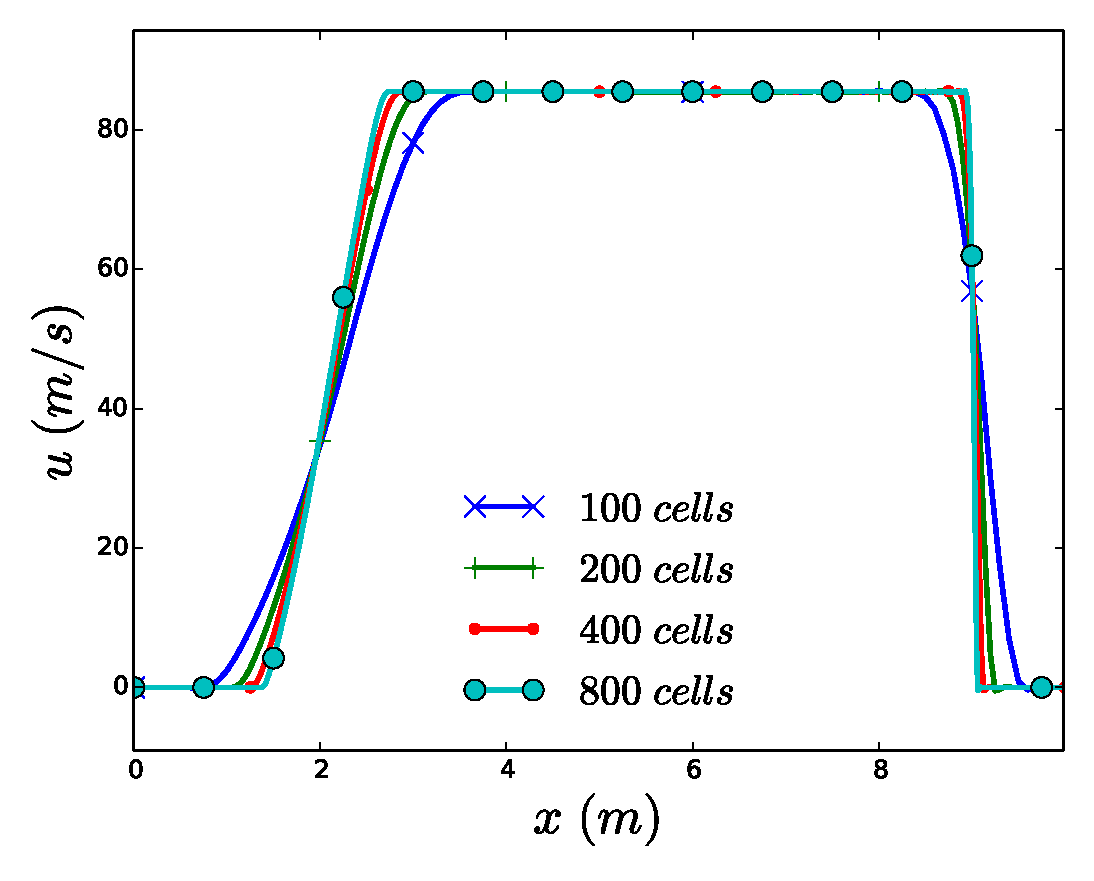
\includegraphics[width=\textwidth]{figures/air-shock-tube-velocity-plot.eps}
                \caption{Velocity}
                \label{fig:air-tube-plots-vel}
        \end{subfigure}%
        \begin{subfigure}[b]{0.5\textwidth}
                \centering
                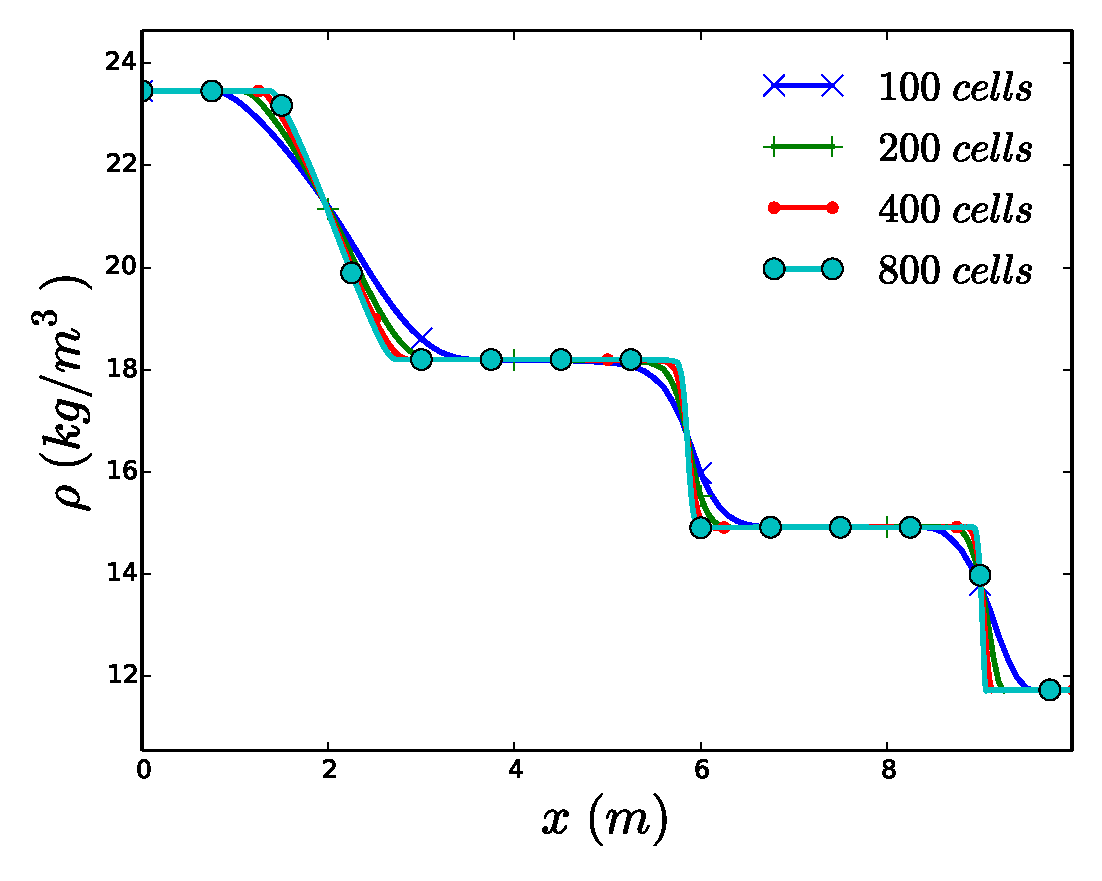
\includegraphics[width=\textwidth]{figures/air-shock-tube-density-plot.eps}
                \caption{Density}
                \label{fig:air-tube-plots-dens}
        \end{subfigure}
        
        \begin{subfigure}[b]{0.495\textwidth}
                \centering
                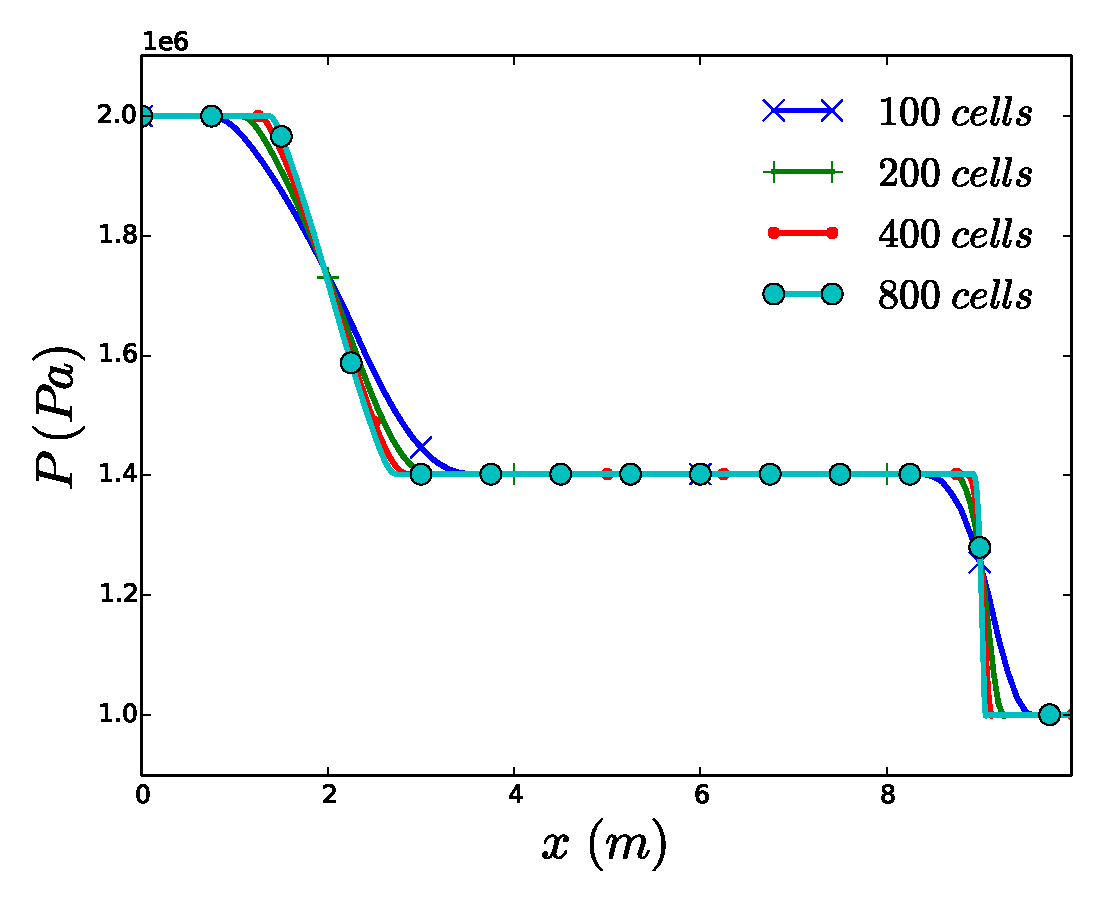
\includegraphics[width=\textwidth]{figures/air-shock-tube-pressure-plot.eps}
                \caption{Pressure}
                \label{fig:air-tube-plots-press}
        \end{subfigure}        
        \begin{subfigure}[b]{0.495\textwidth}
                \centering
                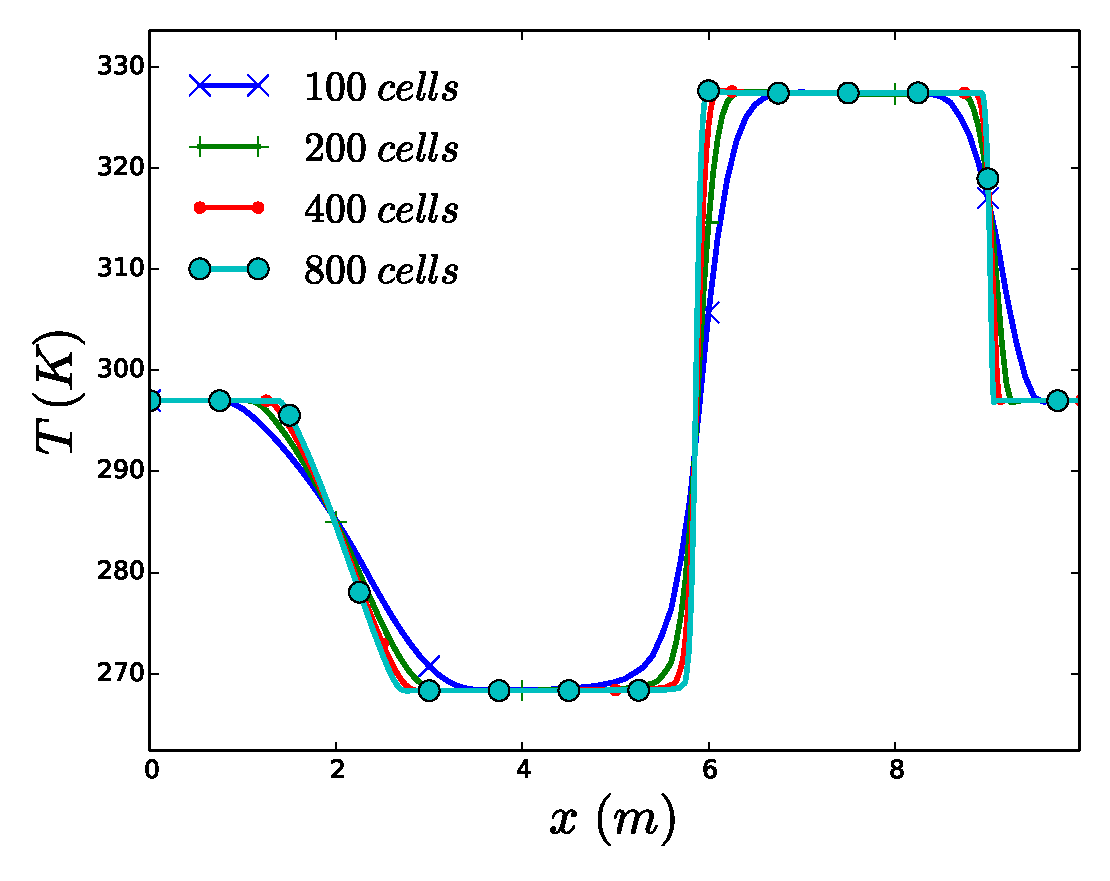
\includegraphics[width=\textwidth]{figures/air-shock-tube-temperature-plot.eps}
                \caption{Temperature}
                \label{fig:air-tube-plots-temp}
        \end{subfigure}
        \caption{Numerical solutions of an air shock tube at $t=10^{-2} \ s$ for mesh with $100$, $200$, $400$ and $800$ cells.}\label{fig:air-tube-plots}
\end{figure}
%
The velocity, density, pressure and temperature profiles are shown in \figs{fig:air-tube-plots-vel} to \ref{fig:air-tube-plots-temp} for different mesh sizes. The contact ($x  \simeq 6 \ m$) and shock ($x  \simeq 9 \ m$) waves do not display any instabilities, are better resolved as the mesh is refined and compare well against the numerical solutions obtained with RELAP-5 and presented in Section 2.1 of \cite{Sokolowski-Koszela}. To investigate the influence of the CFL condition on the numerical solution, the air shock tube test is run on mesh of $200$ cells with three different CFL conditions, $0.1$, $0.5$ and $1.0$. Numerical results of the density are presented in \fig{fig:air-tube-conv-plots-dens} and shown that a CFL condition ranging from $0.1$ to $1$ does not have significant effect on the numerical solution besides the presence of an overshoot in the shock area for CFL $=1.0$. The EVM adds the right amount of dissipation to the solution to stabilize it. In \fig{fig:air-tube-conv-plots-vel}, the air shock tube test is run with the EVM and the first-order viscosity (FOV) using a mesh of $200$ cells and a CFL condition of 0.1. The FOV is obtained by setting $\mu(x,t) = \mu_{max}(x,t)$ in \eqt{eq:single-visc-def-mu} and is known to be over-dissipative whereas the EVM is designed to achieve high-order accuracy with smooth solutions and stabilize a shock wave without smoothing a contact wave. In \fig{fig:air-tube-conv-plots-vel}, the contact and the shock waves are better resolved when using the EVM; the solution obtained with the FOV over-dissipates both the contact and the shock waves.
%
\begin{figure}[H]
    \centering
    \begin{subfigure}[b]{0.49\textwidth}
            \centering
            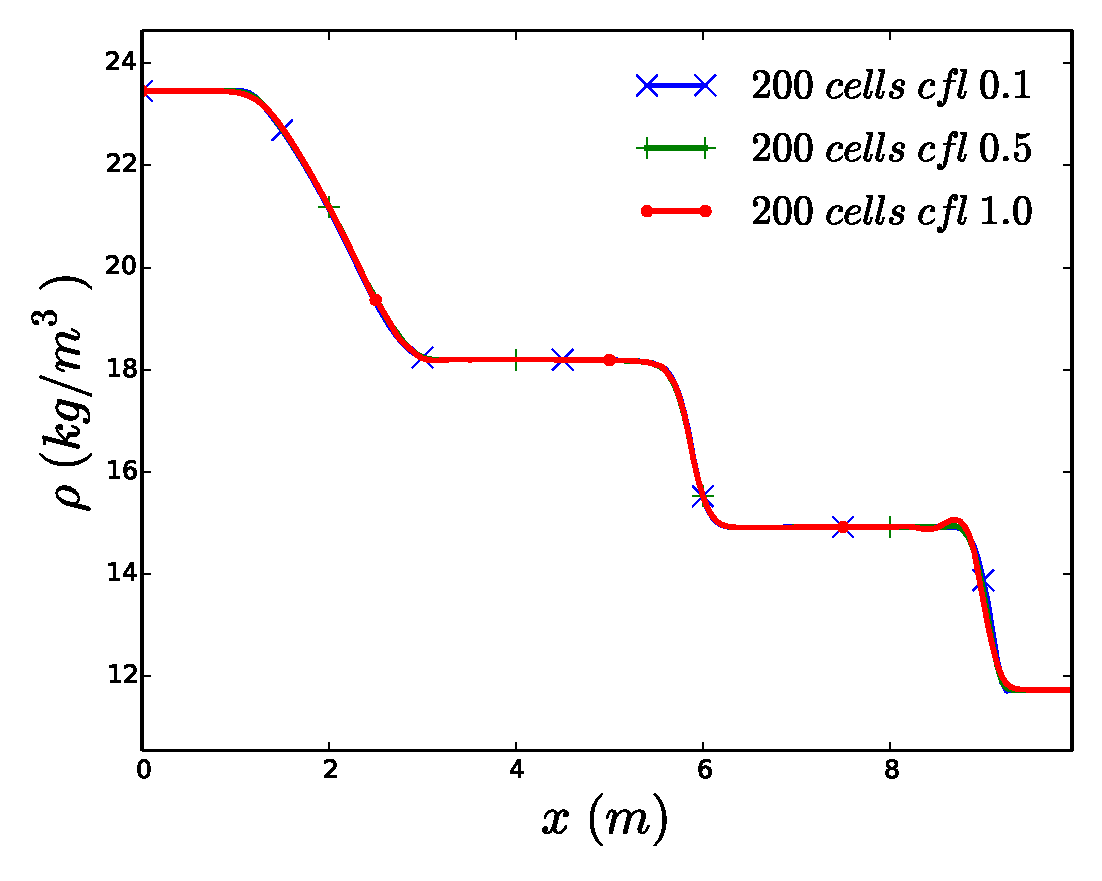
\includegraphics[width=\textwidth]{figures/air-shock-tube_out_displaced-200-cells-cfl-1-0-pts0-density-plot.eps}
            \caption{}
            \label{fig:air-tube-conv-plots-dens}
    \end{subfigure}
    \begin{subfigure}[b]{0.49\textwidth}
            \centering
            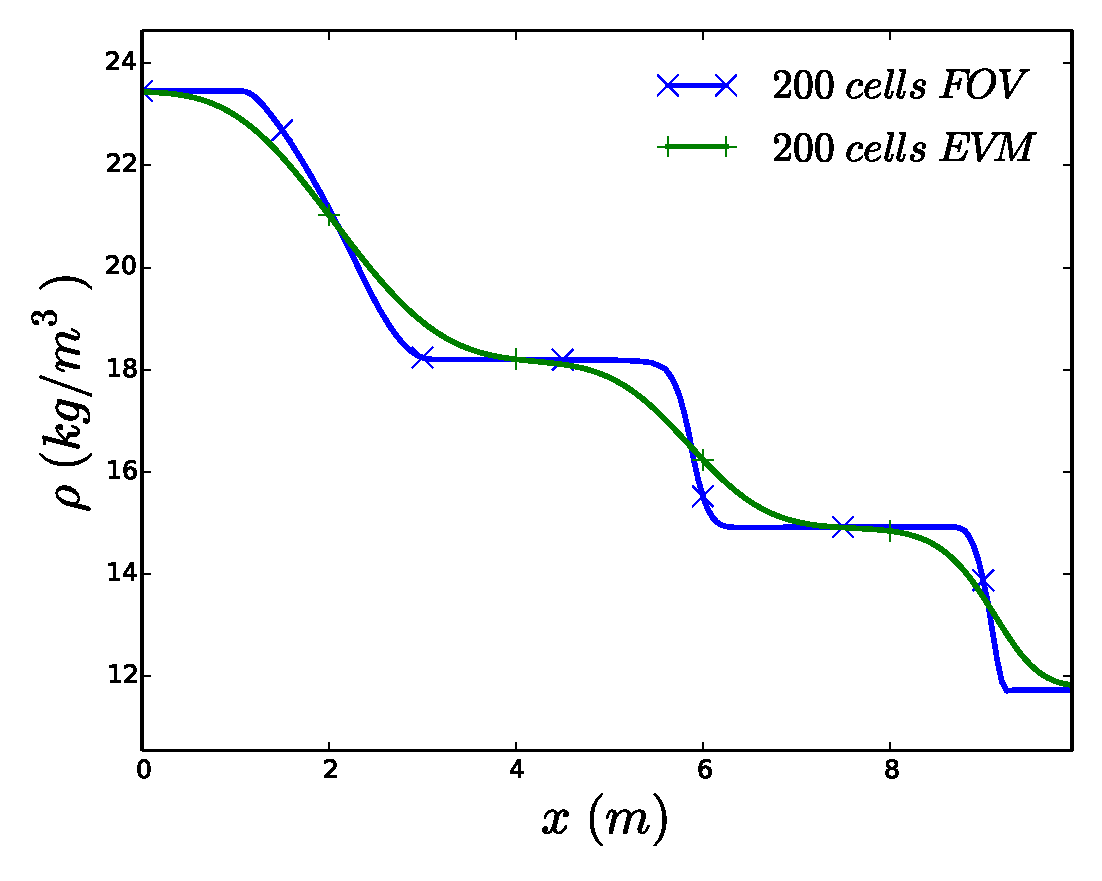
\includegraphics[width=\textwidth]{figures/air-shock-tube_out_displaced-200-cells-cfl-0-1-fo-pts0-density-plot.eps}
            \caption{}
            \label{fig:air-tube-conv-plots-vel}
    \end{subfigure}%
    \caption{Density profile of an air shock tube at $t=10^{-2} \ s$ for mesh with $200$ cells.}\label{fig:air-tube-conv-plots}
\end{figure}    
%
%---------------------------------------------------------------------------------------------------
\subsubsection{Vapor shock tube problem} \label{sec:vap-1-phase-shock-tube}
%---------------------------------------------------------------------------------------------------
%
%\tcb{correct IAPWS in the paper and add details about the bcs} \\
The second test consists of a single-phase vapor shock tube in a pipe of length $L=2 \ m$ and was proposed in \cite{waha-manual, Sokolowski-Koszela}. The 1-D pipe is discretized with a uniform mesh and wall boundary conditions are applied to the left and right ends. A diaphragm located at $x=1 \ m$ separates a high pressure chamber ($P=2 \ MPa$ and $T=486.5 \ K$) and a low pressure chamber ($P=1 \ MPa$ and $T=453.1 \ K$). The vapor properties are computed from the IAPWS95 Spline Based Table Lookup (see section 3.2.7 of \cite{Berry_Peterson_2014}). At $t=0 \ s$, the diaphragm is removed and the vapor initially at rest starts to develop contact, rarefaction and shock waves. The transient is run until $t=1.5 \cdot 10^{-3} \ s$ with a CFL of 0.1. Numerical results are presented in \fig{fig:vapor-tube-plots} for meshes of $100$, $200$, $400$, and $800$ cells.
%
\begin{figure}[H]
        \centering
        \begin{subfigure}[b]{0.5\textwidth}
                \centering
                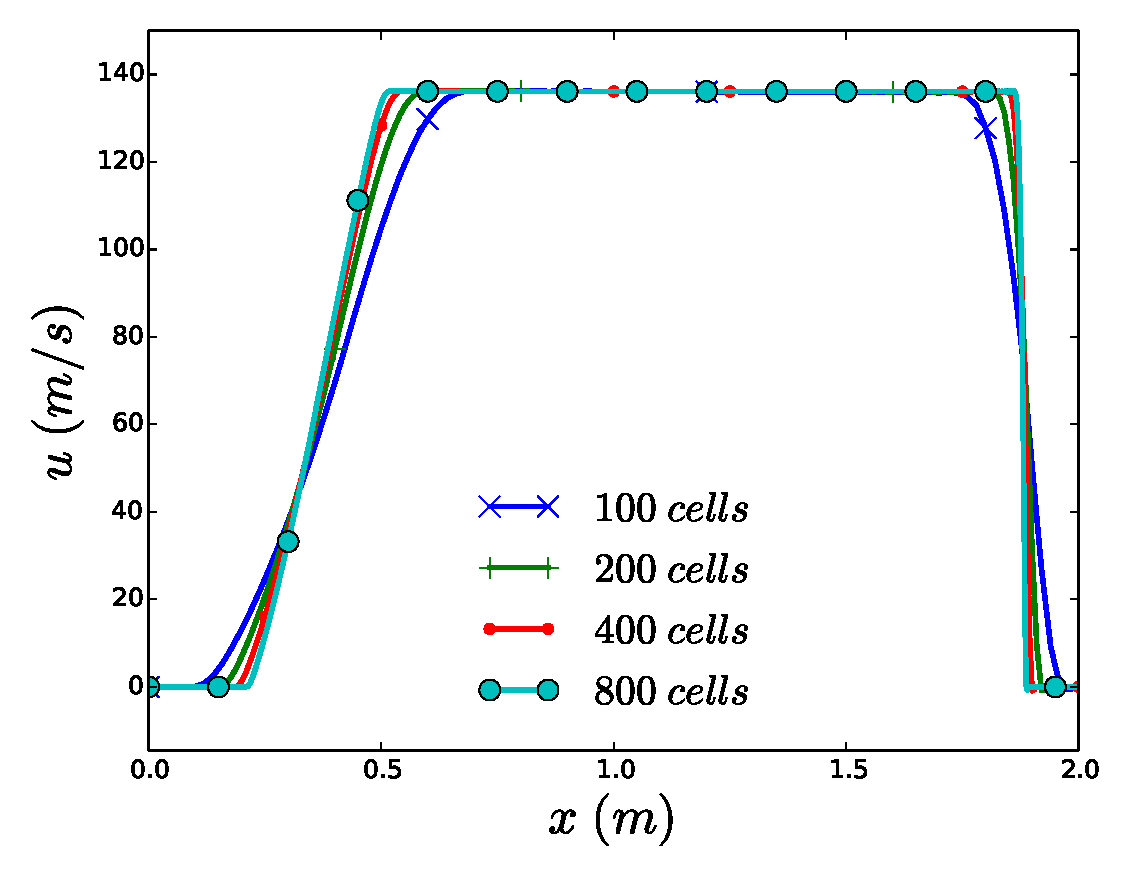
\includegraphics[width=\textwidth]{figures/vapor-mesh-sensitivity-velocity-plot.eps}
                \caption{Velocity}
                \label{fig:vapor-tube-plots-vel}
        \end{subfigure}%
        \begin{subfigure}[b]{0.5\textwidth}
                \centering
                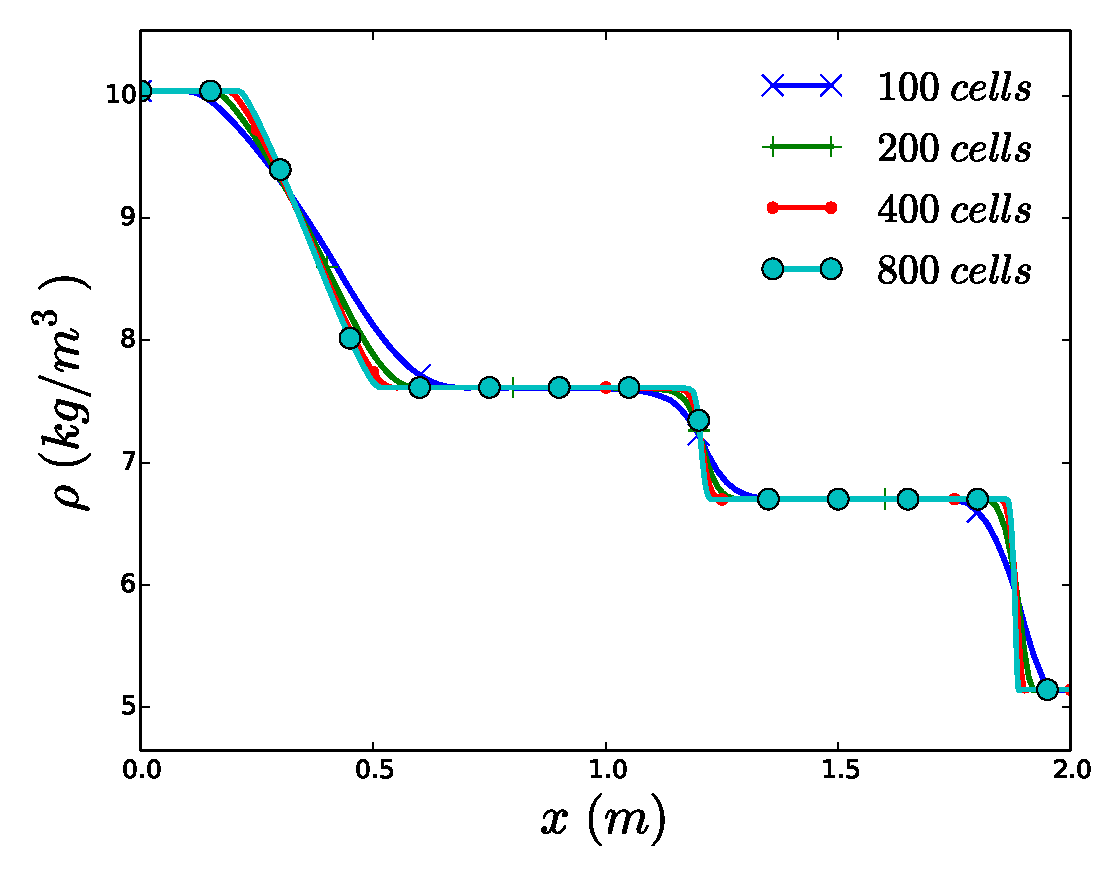
\includegraphics[width=\textwidth]{figures/vapor-mesh-sensitivity-density-plot.eps}
                \caption{Density}
                \label{fig:vapor-tube-plots-dens}
        \end{subfigure}
        
        \begin{subfigure}[b]{0.495\textwidth}
                \centering
                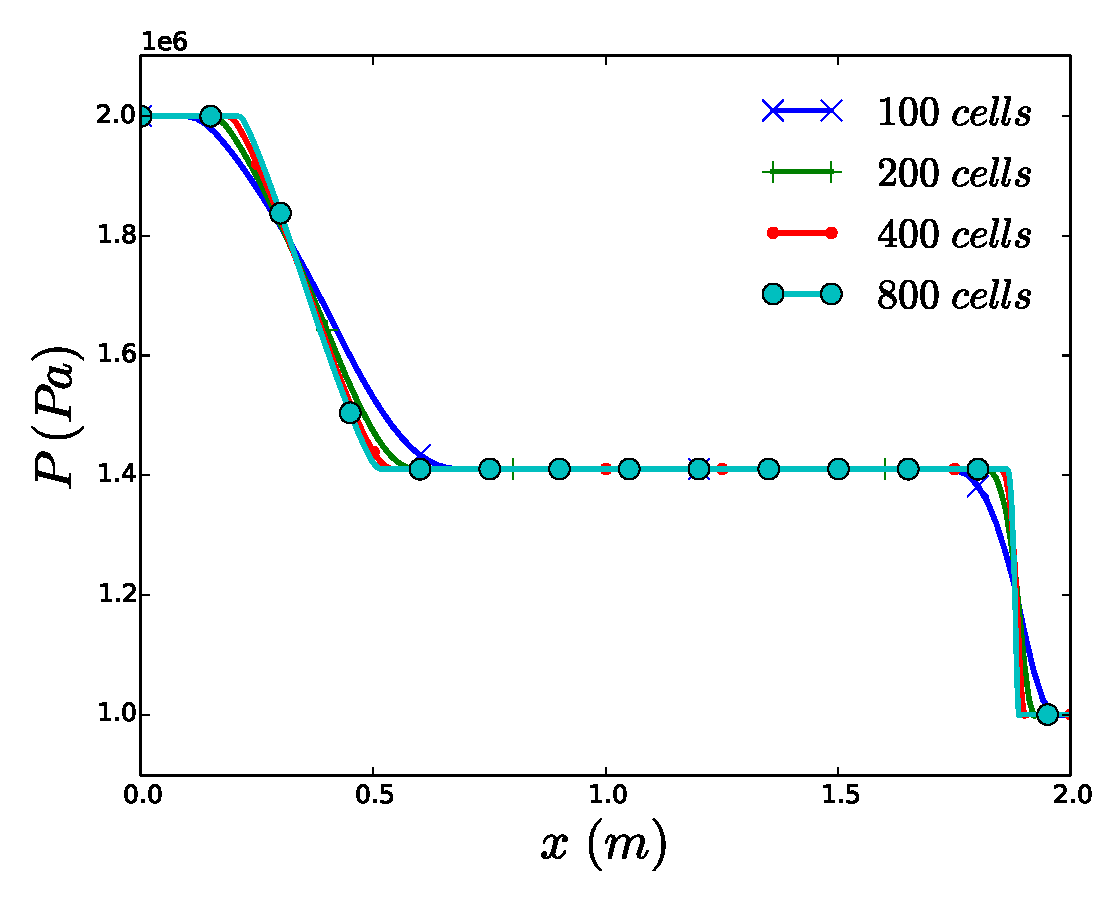
\includegraphics[width=\textwidth]{figures/vapor-mesh-sensitivity-pressure-plot.eps}
                \caption{Pressure}
                \label{fig:vapor-tube-plots-press}
        \end{subfigure}        
        \begin{subfigure}[b]{0.495\textwidth}
                \centering
                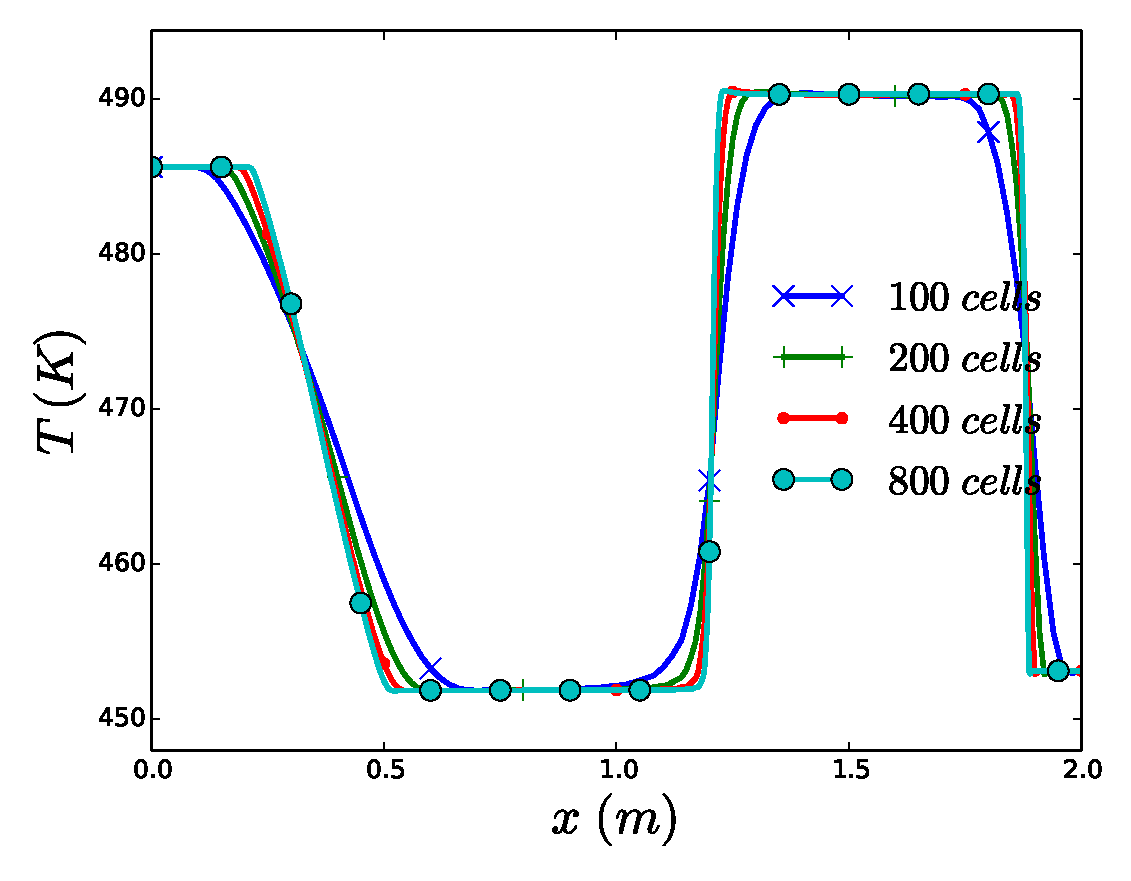
\includegraphics[width=\textwidth]{figures/vapor-mesh-sensitivity-temperature-plot.eps}
                \caption{Temperature}
                \label{fig:vapor-tube-plots-temp}
        \end{subfigure}
        \caption{Numerical solutions of a vapor shock tube at $t=1.5 \cdot 10^{-3} \ s$ for mesh with $100$, $200$, $400$ and $800$ cells.}\label{fig:vapor-tube-plots}
\end{figure}
%
The velocity, density, pressure and temperature profiles are shown in \figs{fig:vapor-tube-plots-vel} to \ref{fig:vapor-tube-plots-temp}. Once again, the numerical solutions do not shown any significant undershoot and overshoot in the contact ($x \simeq 1.2 \ m$) and shock ($x \simeq 1.9 \ m$) regions. The mesh sensitivity analysis of the numerical solution yields the same conclusion as in \sct{sec:air-1-phase-shock-tube}, i.e., the shock and contact waves are better resolved when refining the mesh. The reader can refer to Section 2.2 of \cite{Sokolowski-Koszela} for results of the same vapor shock tube test run with RELAP-5 on a mesh discretized with 200 nodes. The main difference between RELAP-5 and RELAP-7 results lie in the accuracy of the solution in the shock region. The RELAP-5 results display a peak in the post-shock region. The same sensitivity study to the CFL conditions and the numerical method (EVM versus FOV) were performed and yielded the same results as in \sct{sec:air-1-phase-shock-tube}.
%
%---------------------------------------------------------------------------------------------------
\subsubsection{Liquid water shock tube problem} \label{sec:liq-water-1-phase-shock-tube}
%---------------------------------------------------------------------------------------------------
%
In this problem numerical solution of a liquid water shock tube in a pipe of length $L = 10 \ m$ discretized with a uniform mesh is presented. The initial conditions consist of two chambers separated by a diaphragm. The left and right chambers are filled with high ($P=10\ MPa$) and low ($P=0.1\ MPa$) pressure water, respectively. Wall boundary conditions are set to the left and right ends of the 1-D pipe. The water is initially at rest and at the same temperature ($T=300\ K$) in both chambers. The liquid properties are computed from the IAPWS95 Spline Based Table Lookup (see section 3.2.7 of \cite{Berry_Peterson_2014}). At $t=0\ s$, the diaphragm is removed and the flow develops. The transient is run with a CFL condition of 0.1 until $t=1.64 \cdot 10^{-3} \ s$ for mesh with $100$, $200$, $400$, and $800$ cells. This test was previously run with the system code RELAP-5 and the computer code DRAKO \cite{drako} on a mesh discretized with 180 nodes. 
%these results are available in Section 2.3 of \cite{Sokolowski-Koszela}. 
Numerical solutions of the water shock tube test obtained with RELAP-7 are presented in \figs{fig:liquid-tube-plots} at $t=1.64 \cdot 10^{-3} \ s$.
%
\begin{figure}[H]
        \centering
        \begin{subfigure}[b]{0.5\textwidth}
                \centering
                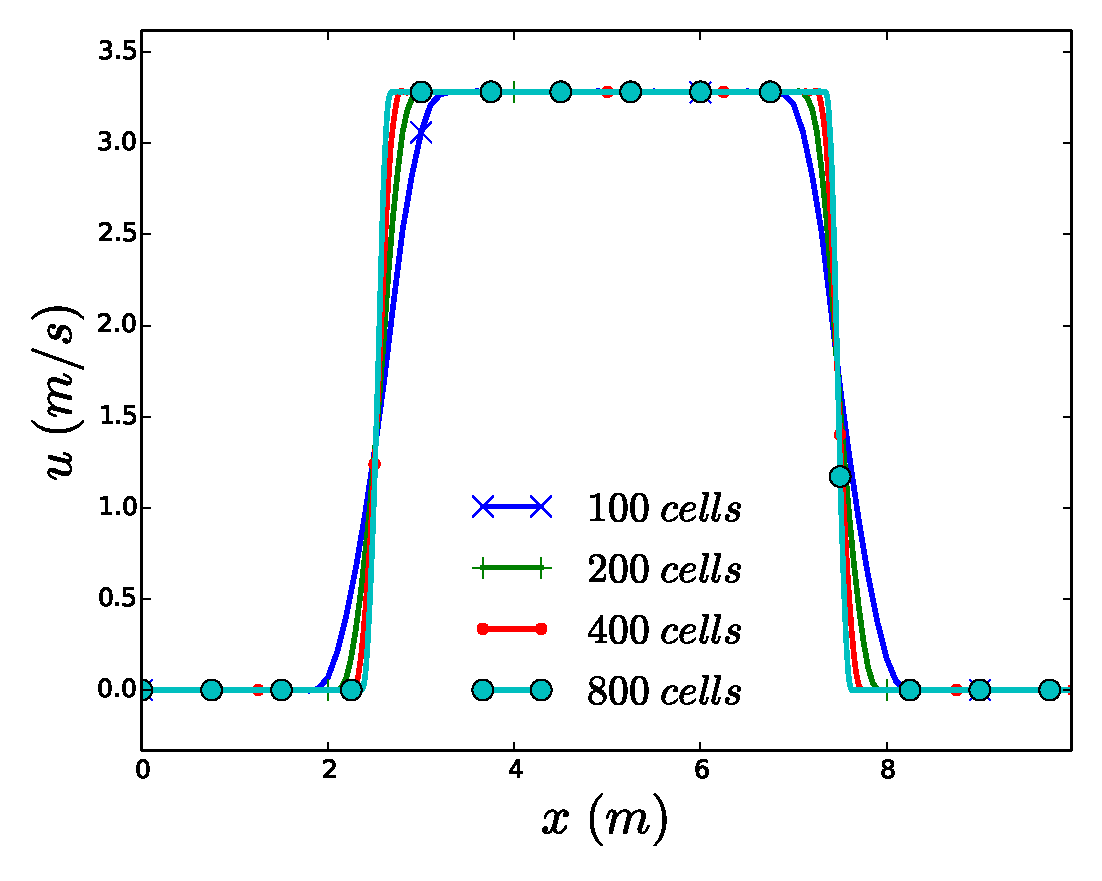
\includegraphics[width=\textwidth]{figures/liquid-mesh-sensitivity-velocity-plot.eps}
                \caption{Velocity}
                \label{fig:liquid-tube-plots-vel}
        \end{subfigure}%
        \begin{subfigure}[b]{0.5\textwidth}
                \centering
                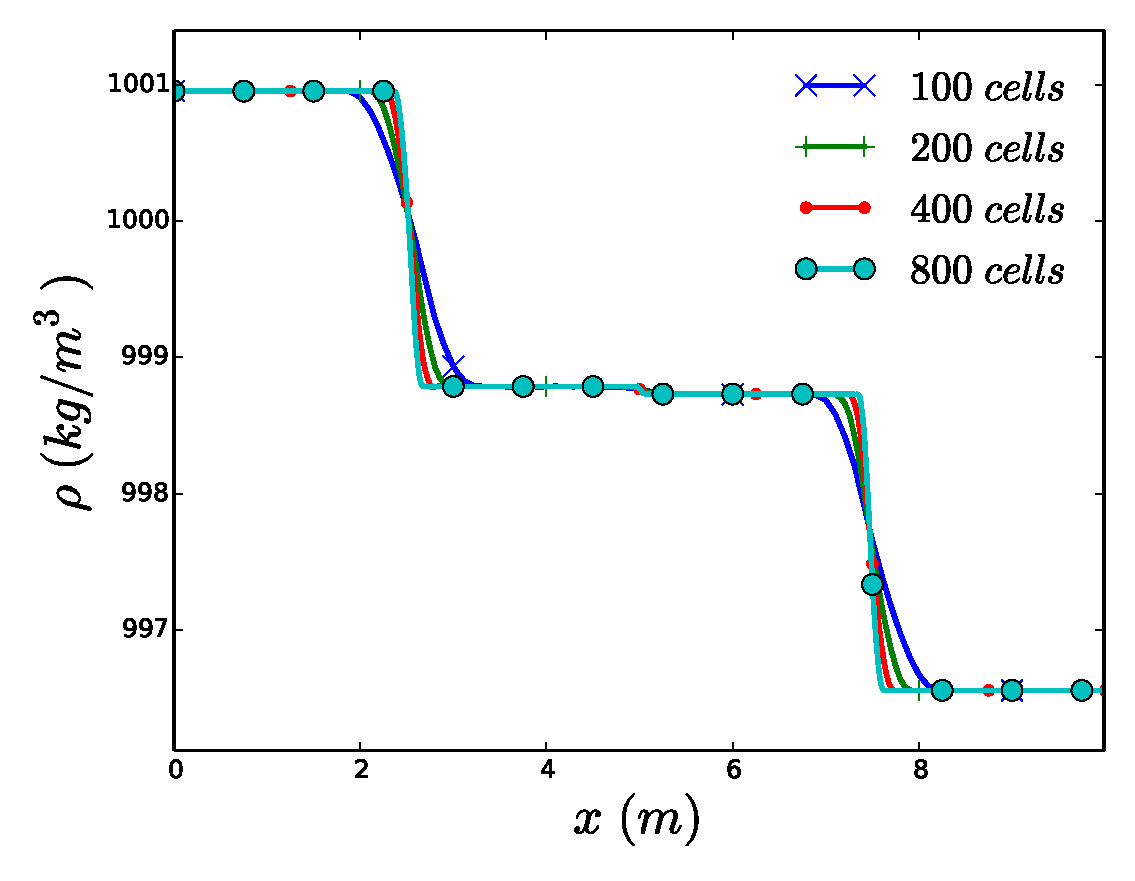
\includegraphics[width=\textwidth]{figures/liquid-mesh-sensitivity-density-plot.eps}
                \caption{Density}
                \label{fig:liquid-tube-plots-dens}
        \end{subfigure}
        
        \begin{subfigure}[b]{0.495\textwidth}
                \centering
                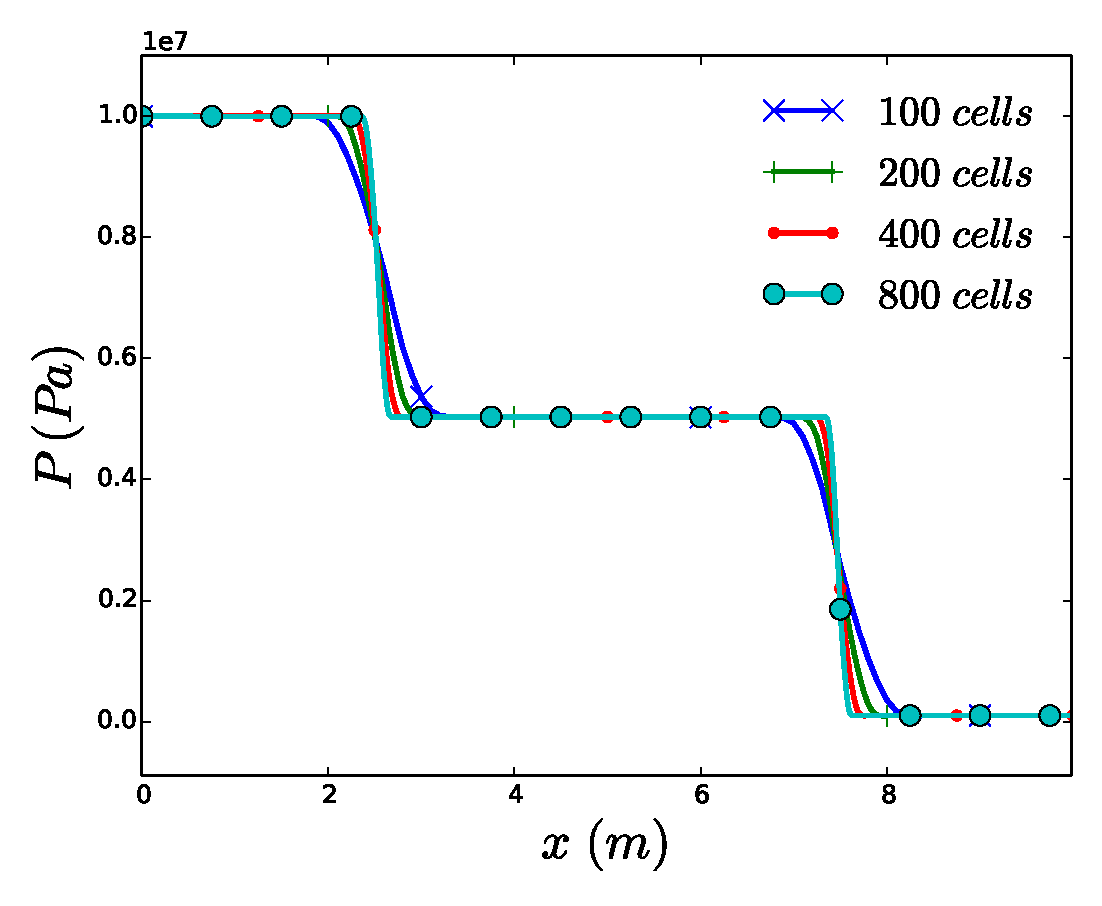
\includegraphics[width=\textwidth]{figures/liquid-mesh-sensitivity-pressure-plot.eps}
                \caption{Pressure}
                \label{fig:liquid-tube-plots-press}
        \end{subfigure}        
        \begin{subfigure}[b]{0.495\textwidth}
                \centering
                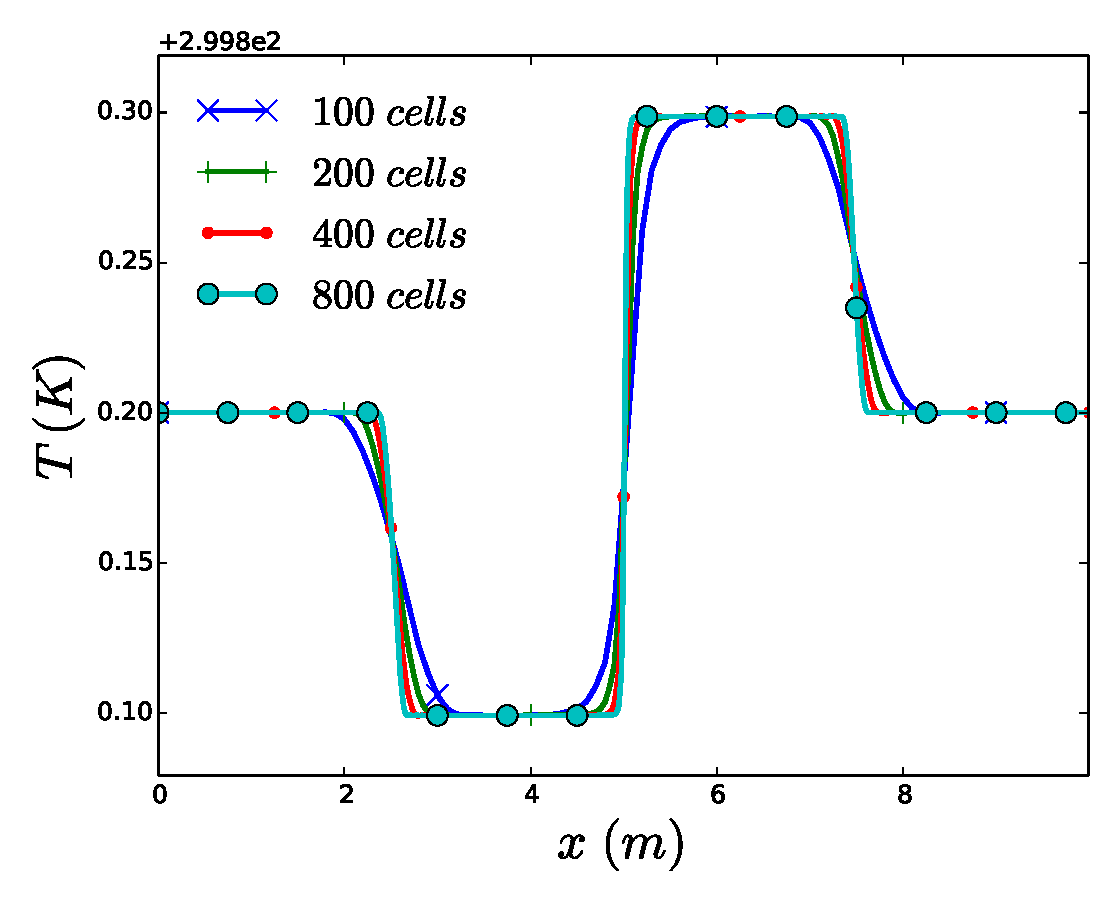
\includegraphics[width=\textwidth]{figures/liquid-mesh-sensitivity-temperature-plot.eps}
                \caption{Temperature}
                \label{fig:liquid-tube-plots-temp}
        \end{subfigure}
        \caption{Numerical solutions of a liquid shock tube at $t=1.64 \cdot 10^{-3} \ s$ for mesh with $100$, $200$, $400$ and $800$ cells.}\label{fig:liquid-tube-plots}
\end{figure}
%
The profiles of the velocity, the density, the temperature and the pressure do not show any instability in the shock ($x \simeq 7.5 \ m$) and contact ($x=\simeq5 \ m$) regions. The discontinuities are better resolved when refining the mesh and do not display significant under- or over-shoots. The numerical solutions presented in \fig{fig:liquid-tube-plots} compare well to the ones obtained with the system code RELAP-5 and the computer code DRAKO shown in Section 2.3 of \cite{Sokolowski-Koszela}. This shock tube test shows the capabilities of the EVM to stabilize liquid water pressure waves.
%
%%---------------------------------------------------------------------------------------------------
%\subsubsection{ Liquid water single-phase water hammer} \label{sec:liq-water-1-phase-hammer}
%%---------------------------------------------------------------------------------------------------
%%
%We now investigate a single-phase liquid water hammer test, i.e. vapor is not generated during the simulation. This test was run with the system code CATHARE \cite{cathare} and results are presented in \cite{Serre-bestion}. The geometry consists of a vertical water tank connected to a horizontal pipe of length L = 36 m and diameter d = 19.05 mm. Initially, the pressure, the temperature and the velocity are uniform and set to P = 3 MPa, V = 0.2786 m/s and T = 488.75 K, respectively. At t = 0 s, a valve is closed at the right end of the pipe, causing a pressure wave to form and travel back and force in the pipe. This test is of interest since the amplitude of the initial over pressure, $\Delta P$ (the pressure simulated at the location of the valve right after it closes), and the period of the phenomenon, $T$, have analytical solutions \cite{Wylie-Streeter-1993}: $\Delta P \simeq \rho c \Delta V = 302633  \ Pa$ and $T = 4 L / c = 0.1125 \ s$ where c is the speed of sound and $\rho$ is the fluid density. These analytical values will be used to compare against the numerical data obtained with the system code RELAP-7. The single-phase liquid water hammer test is run until t = 0.25 s with a CFL of 0.1. The water pressure is monitored at the valve position, i.e. x = 36 m, as a function of time and plotted in \fig{fig:liquid-water-hammer-press-time}.
%\begin{figure}[H]
%        \centering
%        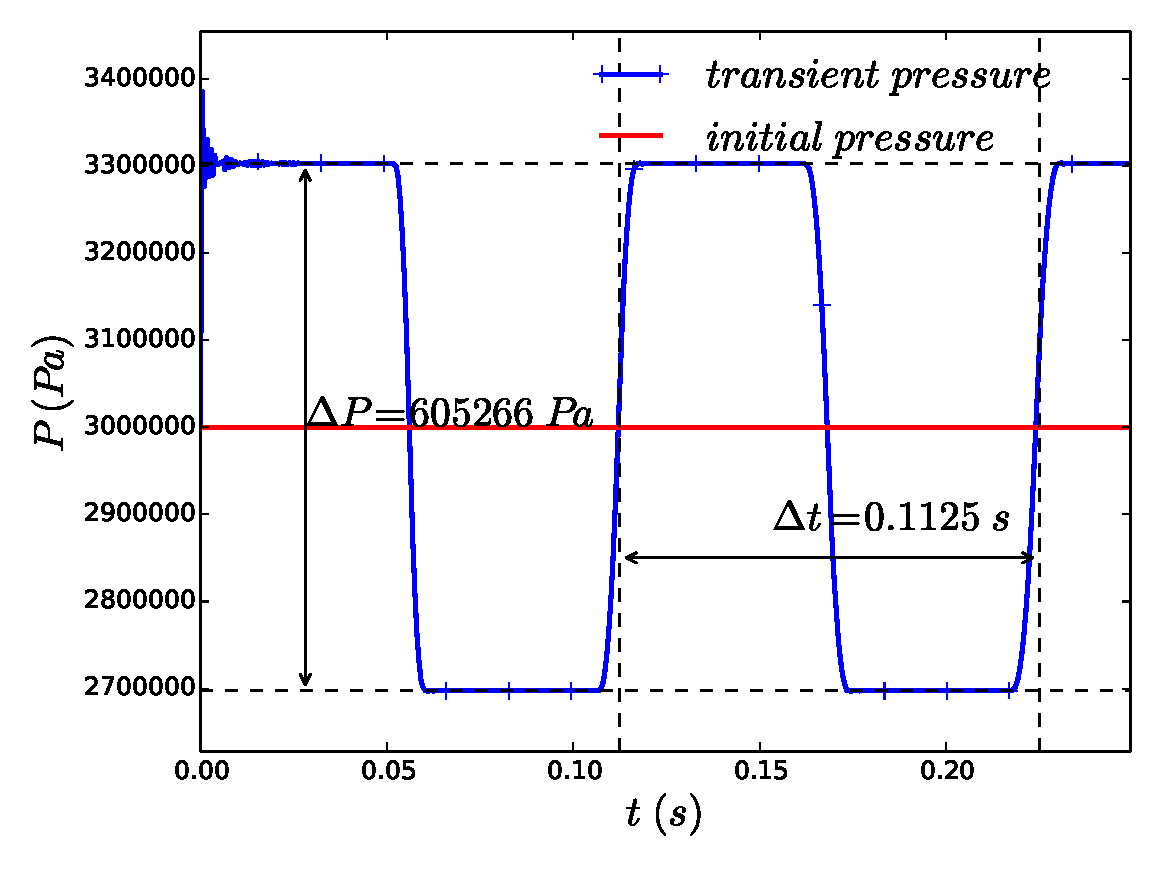
\includegraphics[width=\textwidth]{figures/liquid-water-hammer-pressure-vs-time.eps}
%        \caption{Water pressure as a function of time.}
%        \label{fig:liquid-water-hammer-press-time}
%\end{figure}
%In \fig{fig:liquid-tube-plots-temp}, the water pressure initially increases to stabilize to a value close to 3.3 MPa. The pressure wave travels to the left end of the pipe, is reflected at x = 0 m and travels back to the valve located at x = 36 m. Once, the pressure wave reaches the valve location for the second time, a period is completed and represented by a vertical dashed line at t = 0.1125 s in \fig{fig:liquid-tube-plots-temp} which is in agreement with the analytical value. During this period, the pressure varies between $P_{max} = 3.3 \ MPa$ and $P_{min} = 2.7 \ MPa$.
%

%---------------------------------------------------------------------------------------------------
\subsection{Two-phase test cases} \label{sec:2-phase-problems}
%---------------------------------------------------------------------------------------------------
%
We now present results of a two-phase shock tube obtained with the seven-equation model described in \sct{sec:two-phase-model}. % The EVM is used to stabilize the numerical solution in the presence of shock waves and other discontinuities. 
%Results presented in this section include a two-phase flow shock tube (\sct{sec:2-phase-shock-tube}). 
The objective of this section is to assess the performance of the EVM when simulating two-phase flows developing pressure waves and to recover numerical results previously published in the literature. Once again, all numerical presented in this section are obtained with the RELAP-7 system code and run with linear polynomials as test functions, a second-order Gaussian quadrature rul, and the BDF2 temporal integrator BDF2. \\
%using the RELAP-7 system code implementing the system of equations detailed in \sct{sct:model}. \\
%%
%%---------------------------------------------------------------------------------------------------
%\subsubsection{Two-phase shock tubes} \label{sec:2-phase-shock-tube}
%%---------------------------------------------------------------------------------------------------
%%
We investigate the same two-phase flow shock tube as in \cite{Sokolowski-Koszela, waha-manual}. The geometry is made of a 1-D pipe of length $L = 100\ m$ discretized with an uniform mesh with wall boundary conditions applied to the left and right ends. The initial conditions consist of a left $(P, u, T, \alpha_{vap})_{left} = (15 \ MPa, 0. \ m/s, 615.3 \ K, 0.1)$ and a right $(P, u, T, \alpha_{vap})_{right} = (10 \ MPa, 0. \ m/s, 584.2 \ K, 0.5)$ chamber filled with a mixture of liquid water and vapor. The fluid properties are computed from the IAPWS95 Spline Based Table Lookup (see section 3.2.7 of \cite{Berry_Peterson_2014}). Friction forces are not accounted for in this test. The interfacial area $A_{int}$ used to compute the relaxation parameters $\mu_P$, and $\lambda_u$ defined in \eqt{eq:int_variables_def} is set to $10^6 \ m^{-1}$ which ensures mechanical equilibrium between phases. Because of the very large interfacial area and the mass transfer between the two phases, thermal equilibrium is also achieved. Consequently, under the previous assumptions, the seven-equation model devolves to the homogeneous equilibrium mode (HEM) where the phasic pressures, velocities, and temperatures are equal. It will allow for comparison with the numerical solutions obtained with RELAP-5 \cite{Sokolowski-Koszela} and WAHA \cite{waha-manual} for the same two-phase shock tube as the two codes imply almost immediate mass, momentum and energy inter-phase transfer when using large inter-phase drag and heat transfer coefficients, causing the phasic velocities and temperatures to be nearly identical. 
%\tcr{is this correct that in RELAP-5 the phasic velocities are almost identical?} \tcb{ It is when the drag coefficients is set to a large value.}
%Two sets of simulations are performed. First, the interfacial heat transfer coefficient $h_{int}$ is set to zero while the pressure $\mu_P$ and velocity $\lambda_u$ relaxation coefficients are computed from \eqt{eq:int_variables_def} with $A_{int}=10^6$ and thus large enough to ensure mechanical equilibrium between the two phases, i.e. the phasic velocities and pressures are equal. Under these assumptions, the seven-equation model devolves to the five-equation model of Kapila (REF). This set of simulations is referred to as (1) below. In the second set of simulations, denoted set (2), the interfacial heat transfer coefficient is no longer set to zero but to a value large enough to ensure thermodynamic equilibrium between the two phases, i.e. $T_{vap} = T_{liq}$. The pressure and velocity relaxation parameters are unchanged with respect to the first set of simulations making the seven-equation model devolves to the homogeneous equilibrium model (HEM) (REF). The reader can refer to results of the same test previously obtained with the WAHA code (Section 8.2.1 of \cite{waha-manual}) and with the RELAP-5 system code \cite{Sokolowski-Koszela} for comparison. 
At $t = 0\ s$, the membrane located in the middle of the pipe is removed and the flow develops. The transient is run until $t = 0.081\ s$ with a CFL of 0.1 on successive uniform meshes discretized with 100, 200, and 400 cells. Numerical results obtained with RELAP-7 are showed in \fig{fig:2p-shock-tube-plots-hem-kapila}.
%The same two-phase flow shock tube was previously run with RELAP-5 and WAHA system codes in \cite{Sokolowski-Koszela, waha-manual}. 
%We first present a comparison between (1) and (2) for meshes discretized with 100 elements in \fig{fig:2p-shock-tube-plots}. 
%Then, a mesh sensitivity analysis is performed for each case, i.e. (1) and (2), and numerical results of the phasic volume fractions and densities are presented in \fig{fig:2p-shock-tube-plots-hem-kapila-sa}.
%%
%\begin{figure}[H]
%        \vspace{-1 mm}
%        \centering
%        \begin{subfigure}[b]{0.49\textwidth}
%                \centering
%%                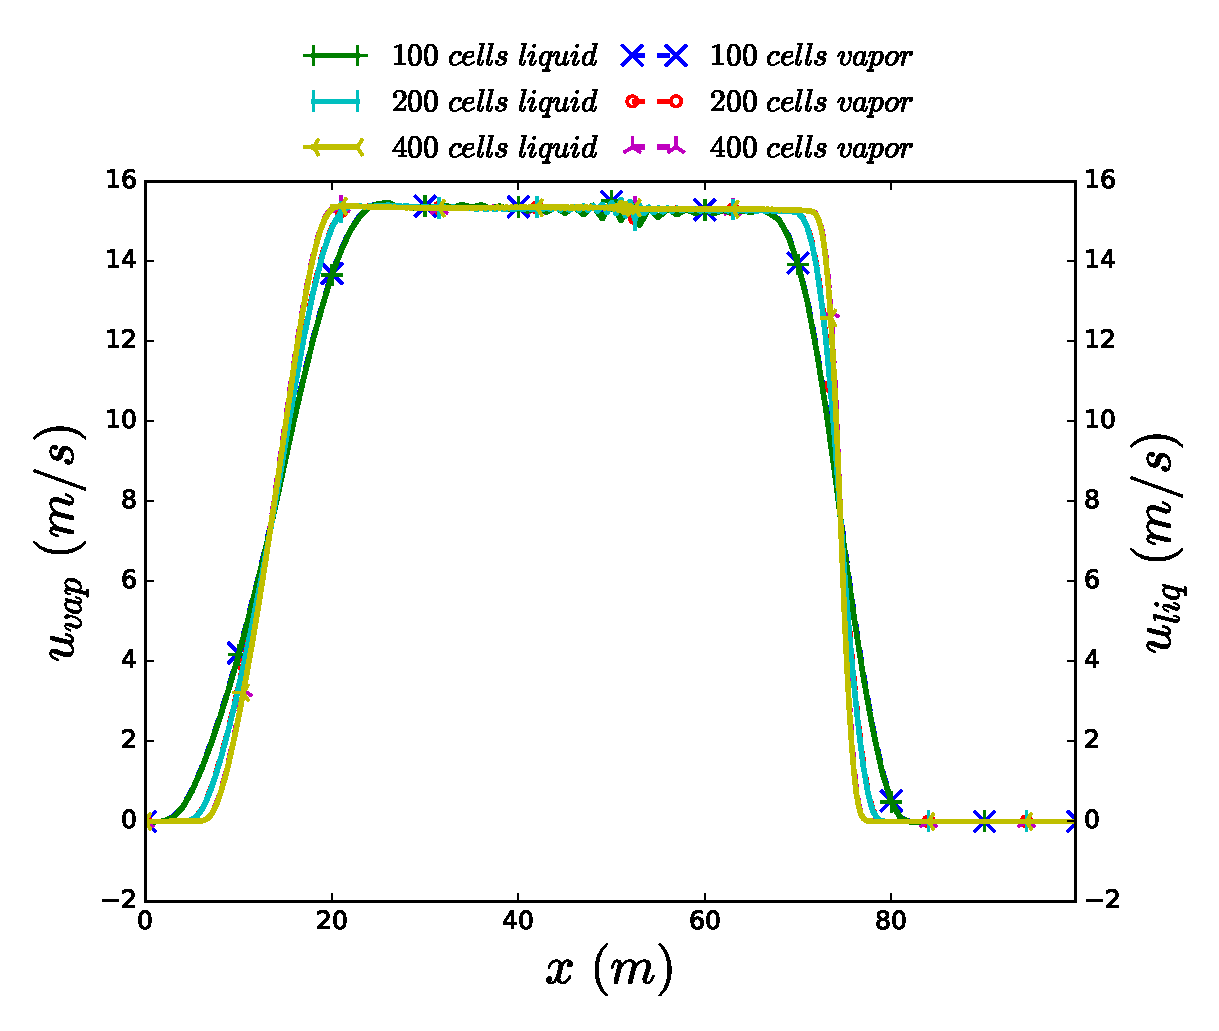
\includegraphics[width=\textwidth]{figures/two-phase-shock-tube-velocity-plot.eps}
%                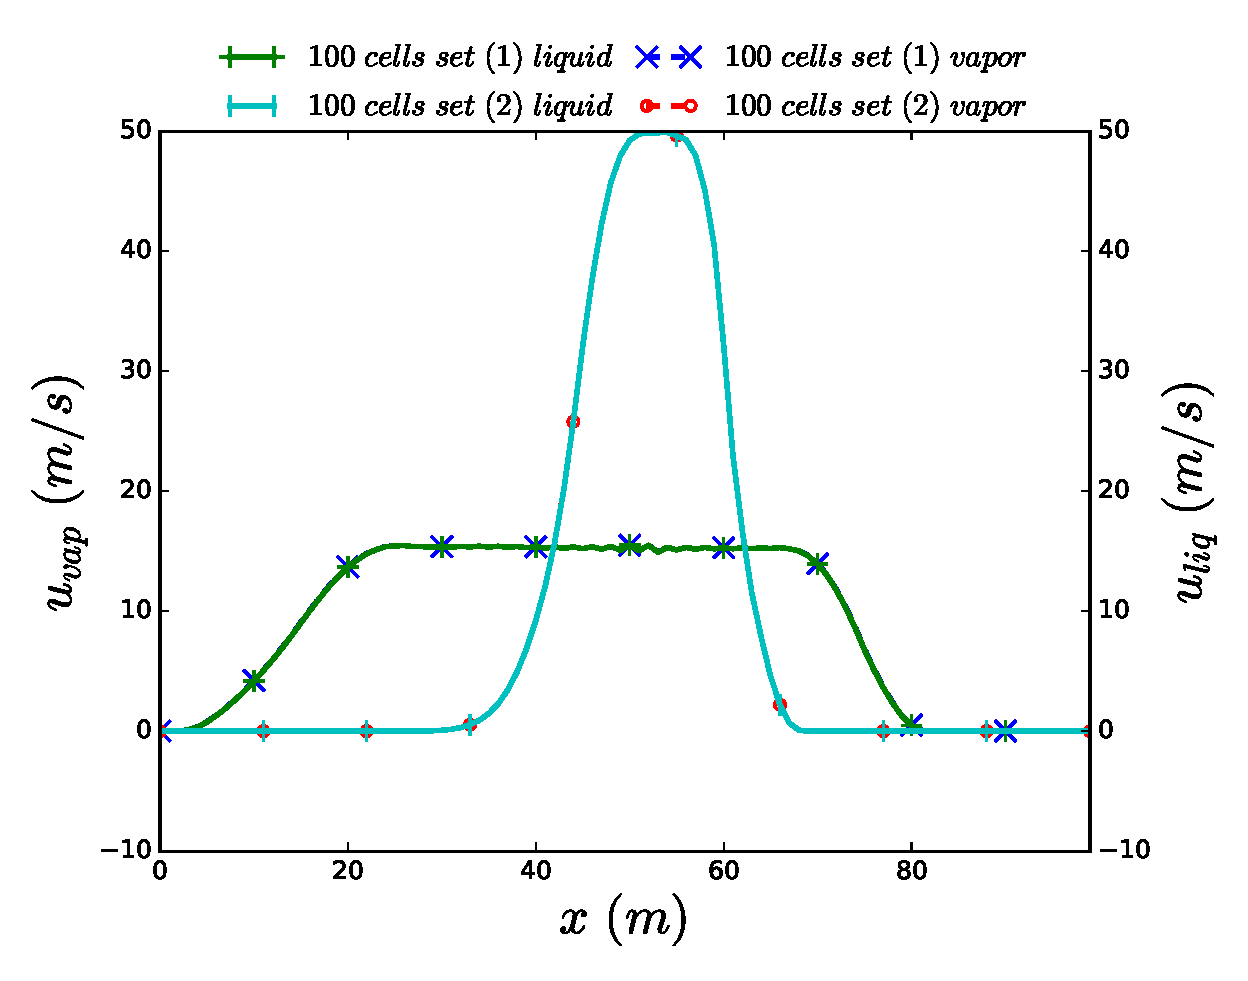
\includegraphics[width=\textwidth]{figures/hem-vs-kapil-100-velocity-plot.eps}                
%                \caption{Velocity}
%                \label{fig:2p-shock-tube-plots-vel}
%        \end{subfigure}%
%        \begin{subfigure}[b]{0.49\textwidth}
%                \centering
%                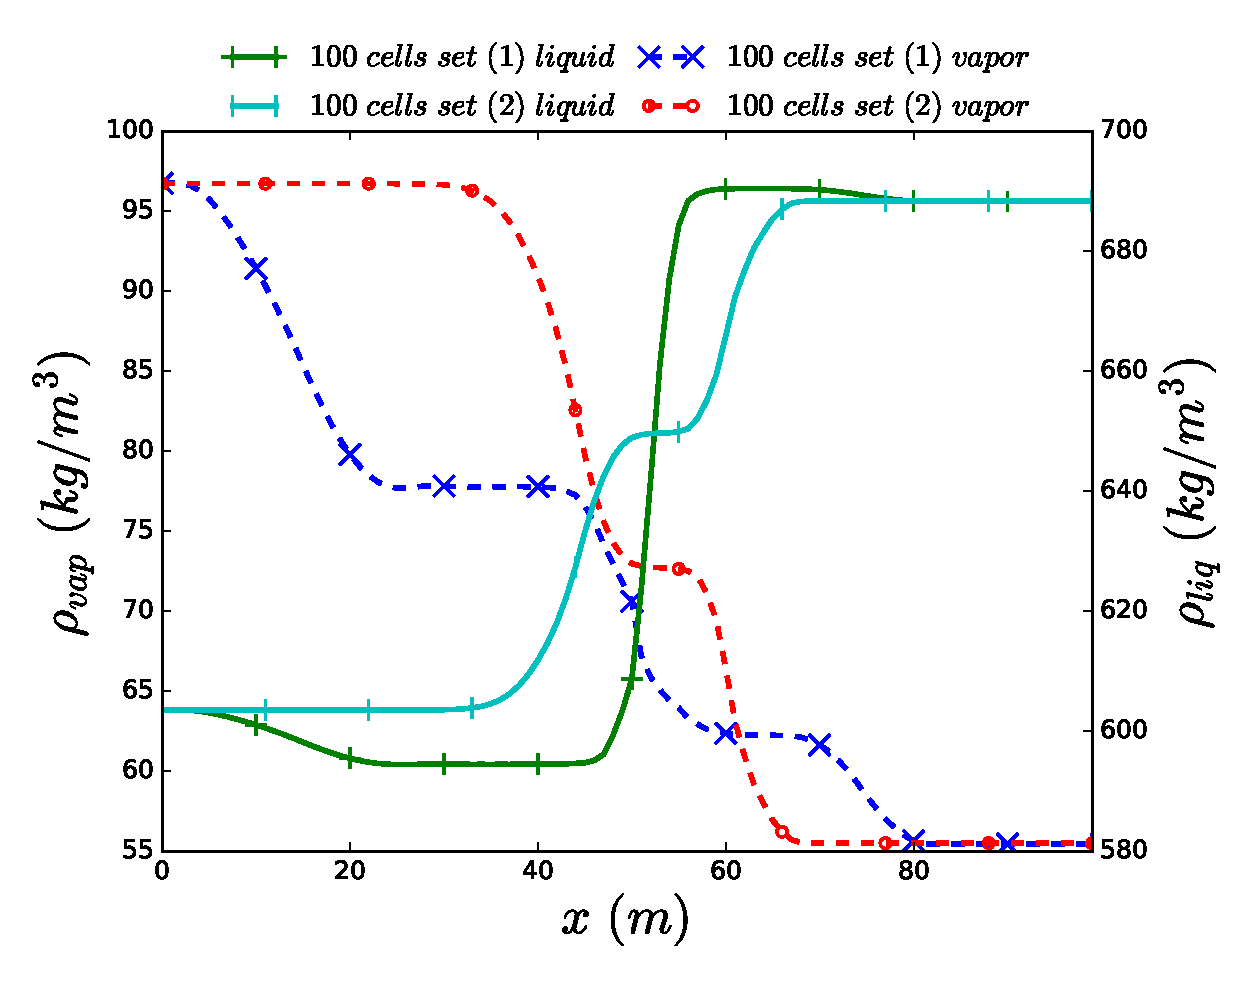
\includegraphics[width=\textwidth]{figures/hem-vs-kapil-100-density-plot.eps}              
%                \caption{Density}
%                \label{fig:2p-shock-tube-plots-dens}
%        \end{subfigure}
%        \vspace{-1 mm}
%        
%        \begin{subfigure}[b]{0.49\textwidth}
%                \centering
%                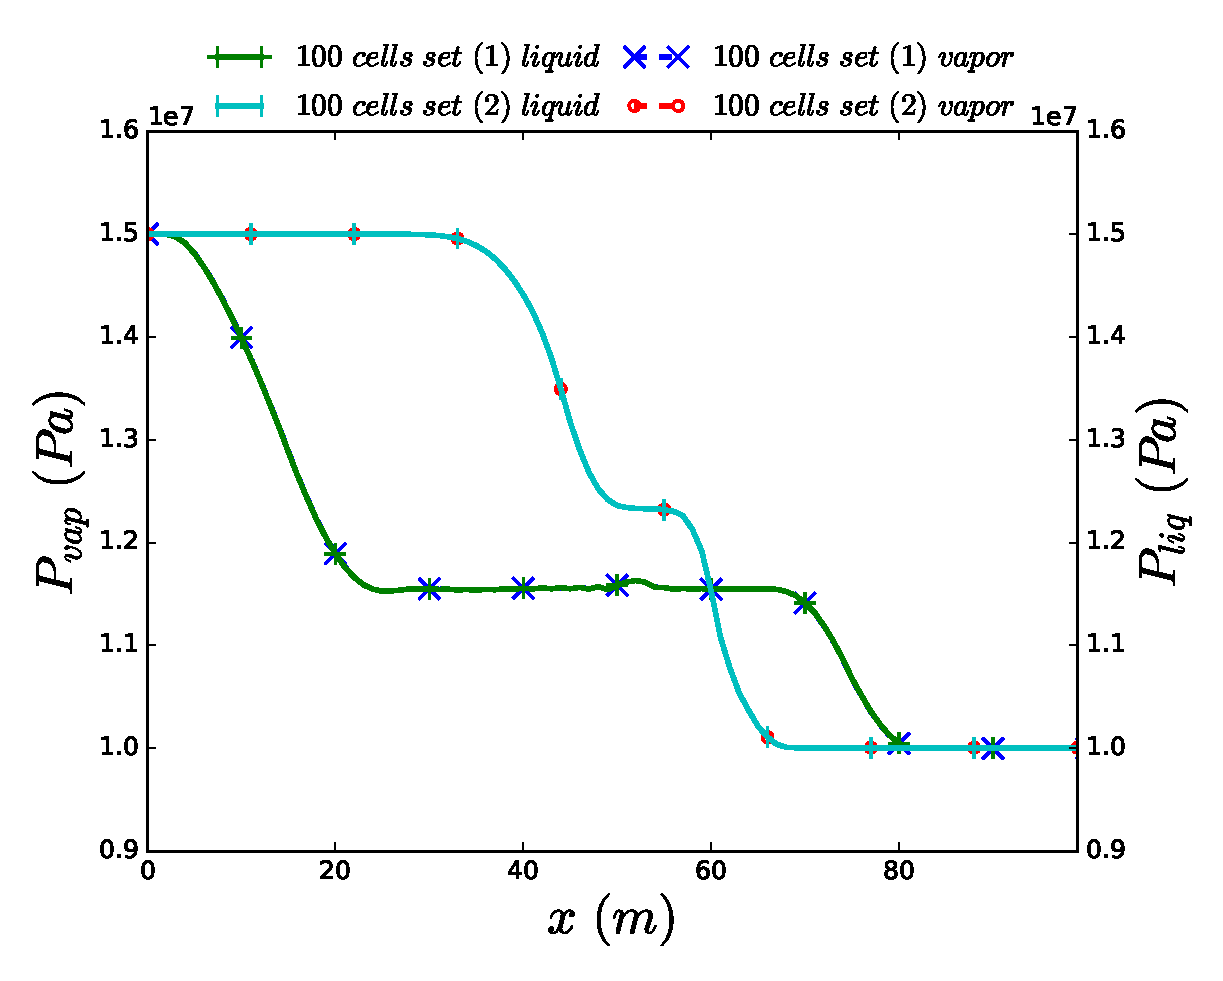
\includegraphics[width=\textwidth]{figures/hem-vs-kapil-100-pressure-plot.eps}
%                \caption{Pressure}
%                \label{fig:2p-shock-tube-plots-press}
%        \end{subfigure}        
%        \begin{subfigure}[b]{0.49\textwidth}
%                \centering
%                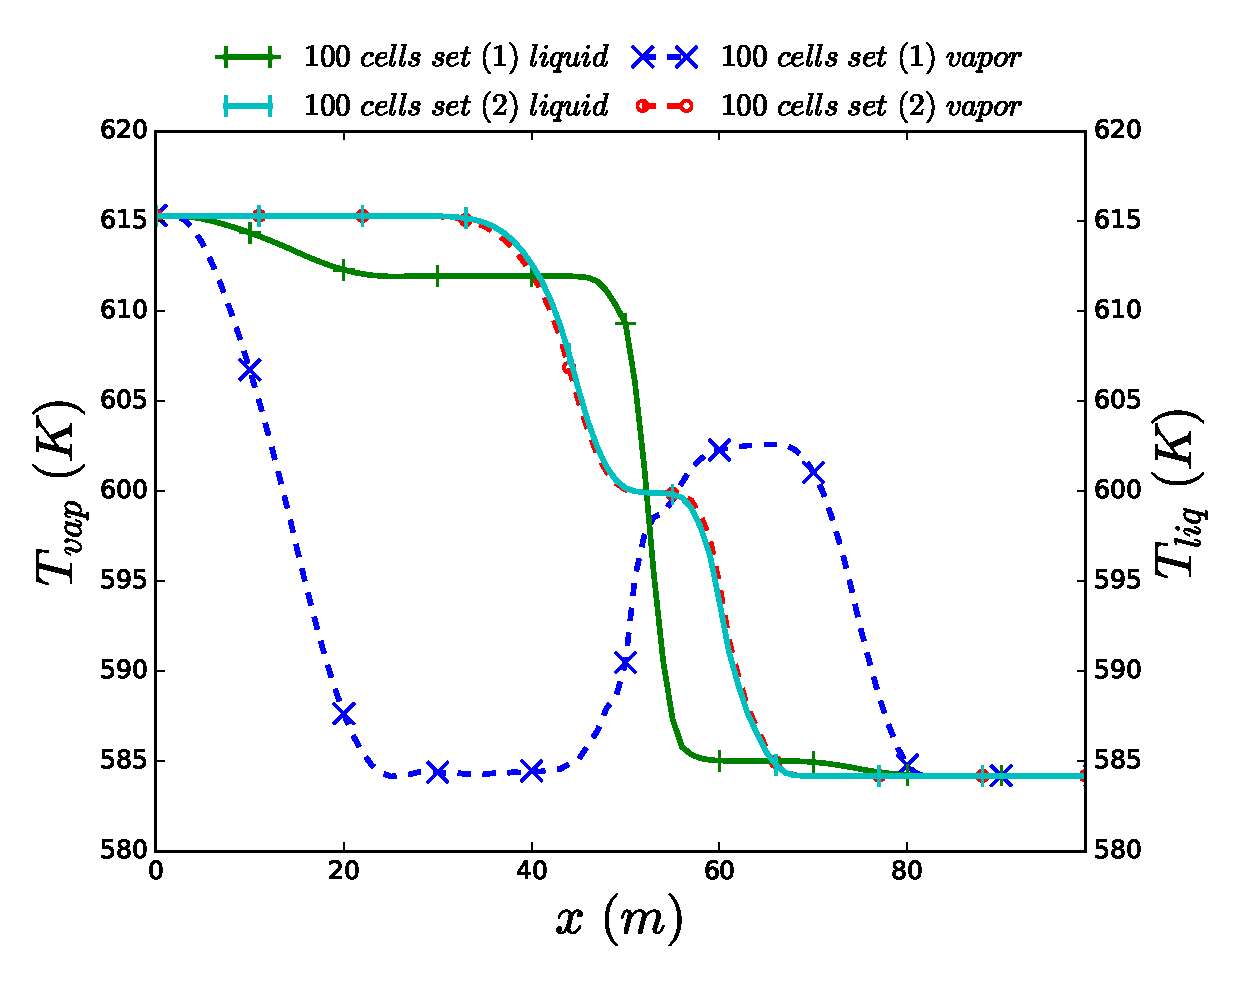
\includegraphics[width=\textwidth]{figures/hem-vs-kapil-100-temperature-plot.eps}
%                \caption{Temperature}
%                \label{fig:2p-shock-tube-plots-temp}
%        \end{subfigure}
%        \vspace{-1.3 mm}        
%        
%        \begin{subfigure}[b]{0.49\textwidth}
%                \centering
%                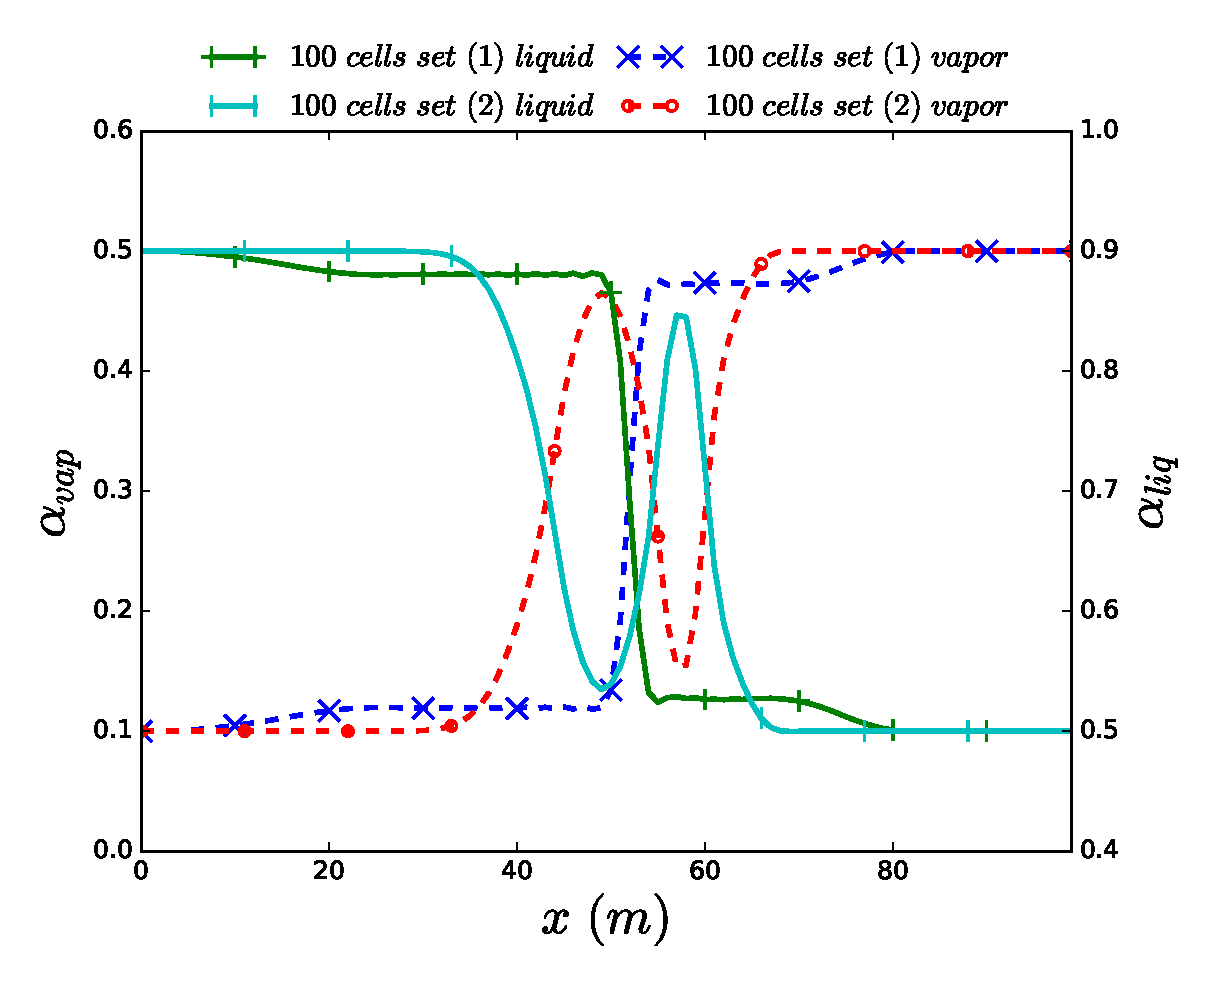
\includegraphics[width=\textwidth]{figures/hem-vs-kapil-100-vf-plot.eps}
%                \caption{Volume fraction}
%                \label{fig:2p-shock-tube-plots-vf}
%        \end{subfigure}                
%        \caption{Numerical solutions of a two-phase flow shock tube at $t=8.1 \cdot 10^{-2} \ s$ for mesh with $100$ cells.}\label{fig:2p-shock-tube-plots}
%\end{figure}
%%
%
\begin{figure}[H]
        \vspace{-1 mm}
        \centering
        \begin{subfigure}[b]{0.49\textwidth}
                \centering
                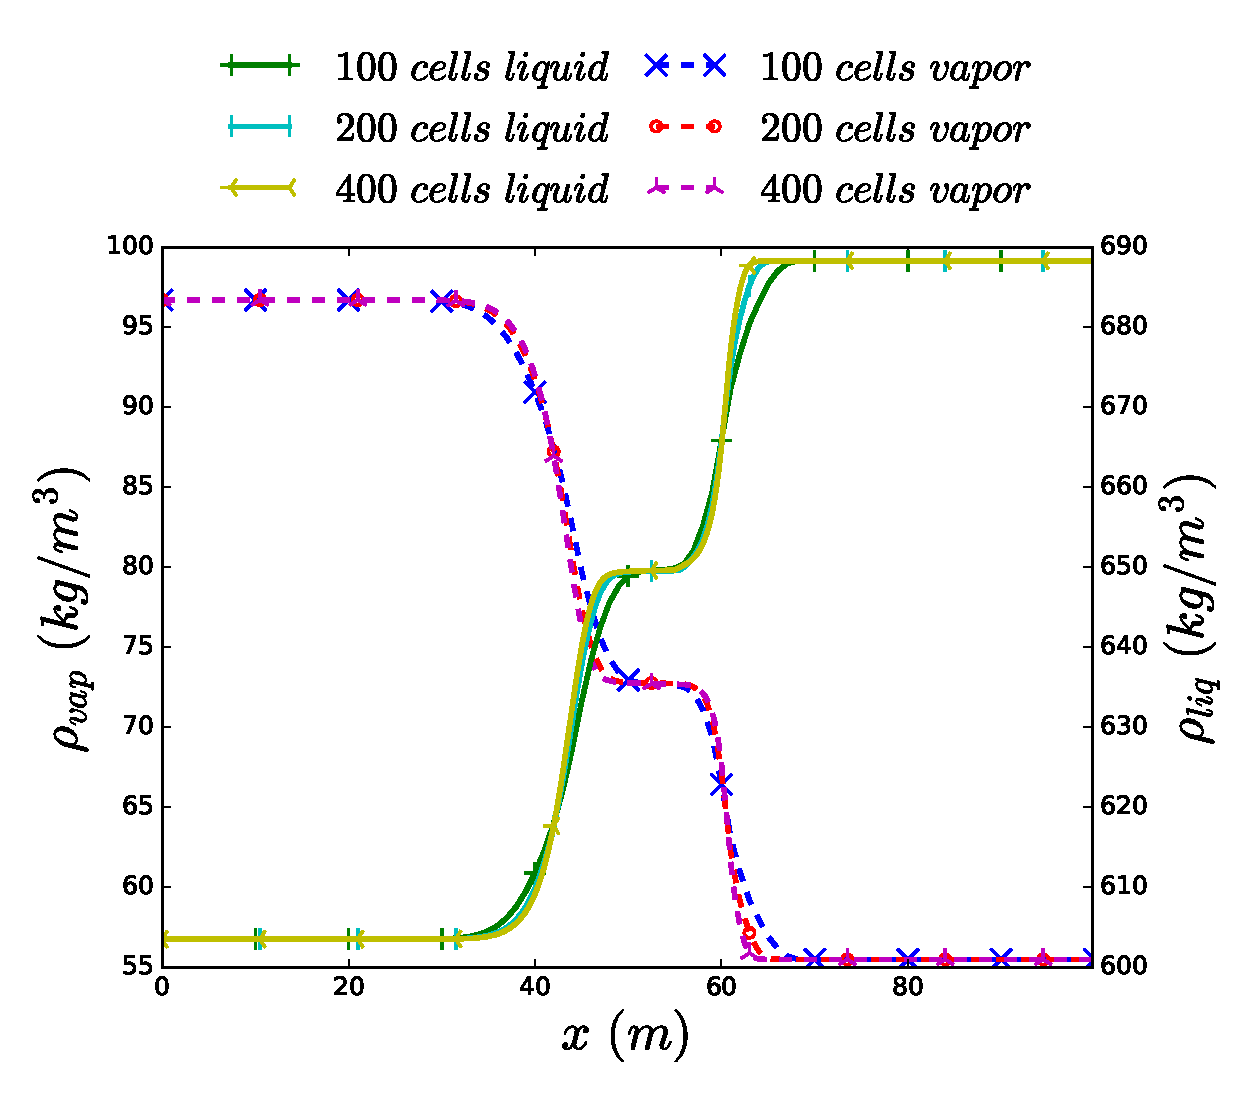
\includegraphics[width=\textwidth]{figures/two-phase-shock-tube-hem-density-plot.eps}                
                \caption{Phasic densities}
                \label{fig:2p-shock-tube-plots-rho-hem-sa}
        \end{subfigure}%
        \begin{subfigure}[b]{0.435\textwidth}
                \centering
                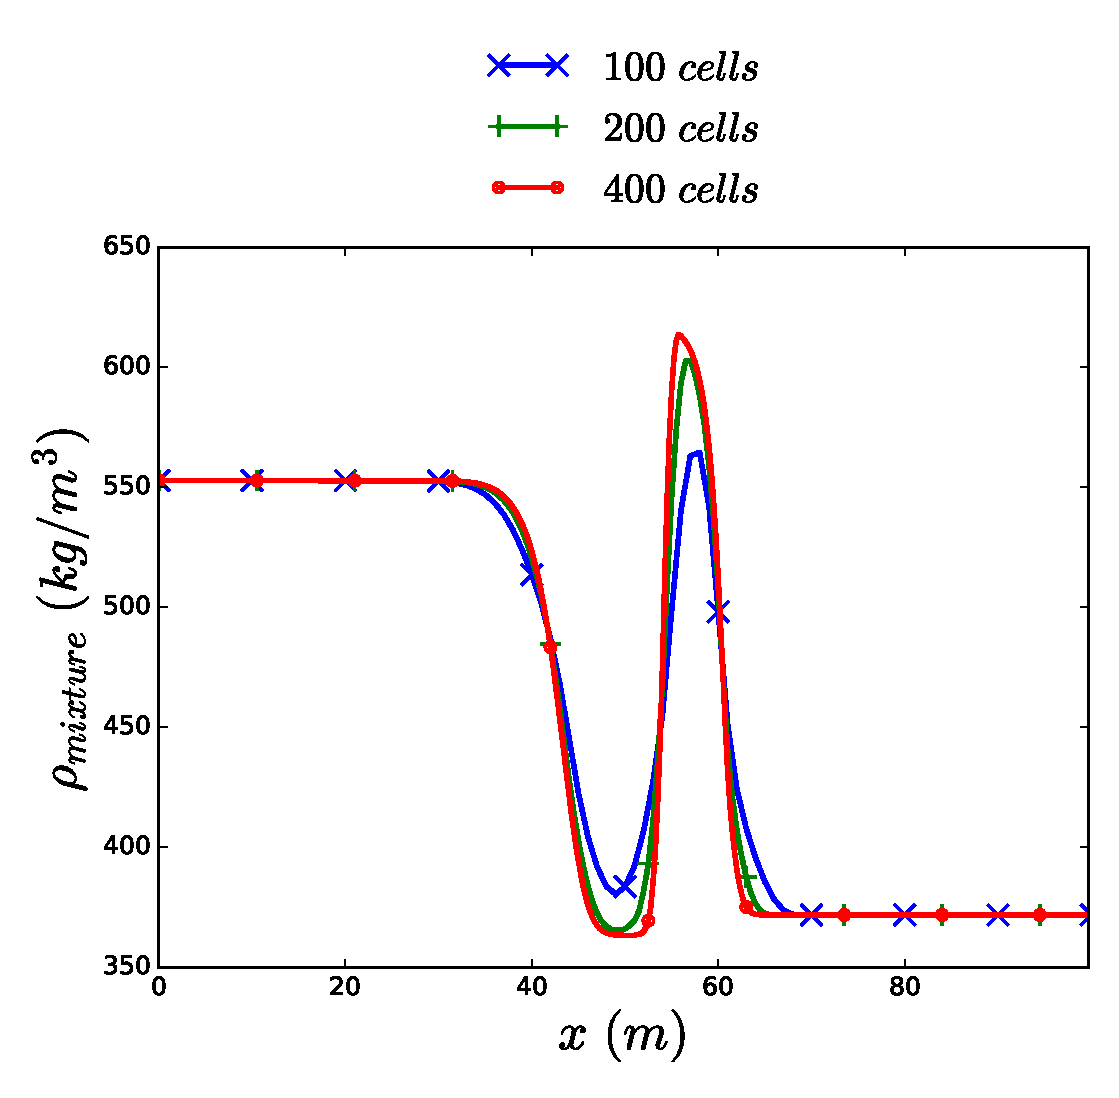
\includegraphics[width=\textwidth]{figures/two-phase-shock-tube-hem-density-mixture-plot.eps}                
                \caption{Mixture density}
                \label{fig:2p-shock-tube-plots-rho-mix-hem-sa}
        \end{subfigure}%        
        
        \begin{subfigure}[b]{0.49\textwidth}
                \centering
                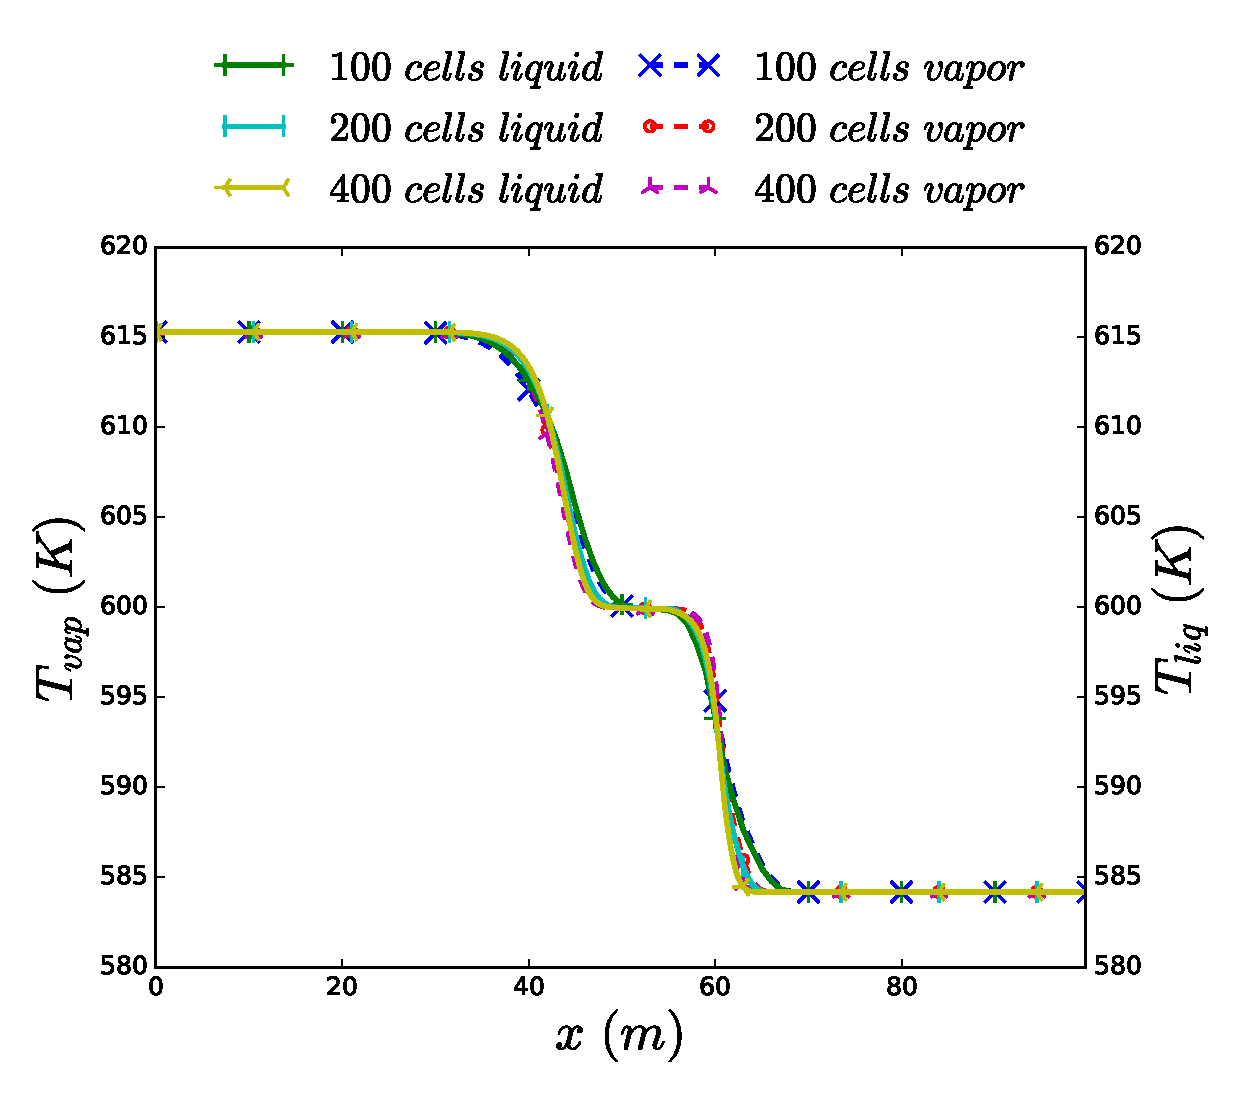
\includegraphics[width=\textwidth]{figures/two-phase-shock-tube-hem-temperature-plot.eps}              
                \caption{Temperature}
                \label{fig:2p-shock-tube-plots-temp-hem-sa}
        \end{subfigure}
        \vspace{-1 mm}
        \centering
        \begin{subfigure}[b]{0.49\textwidth}
                \centering
                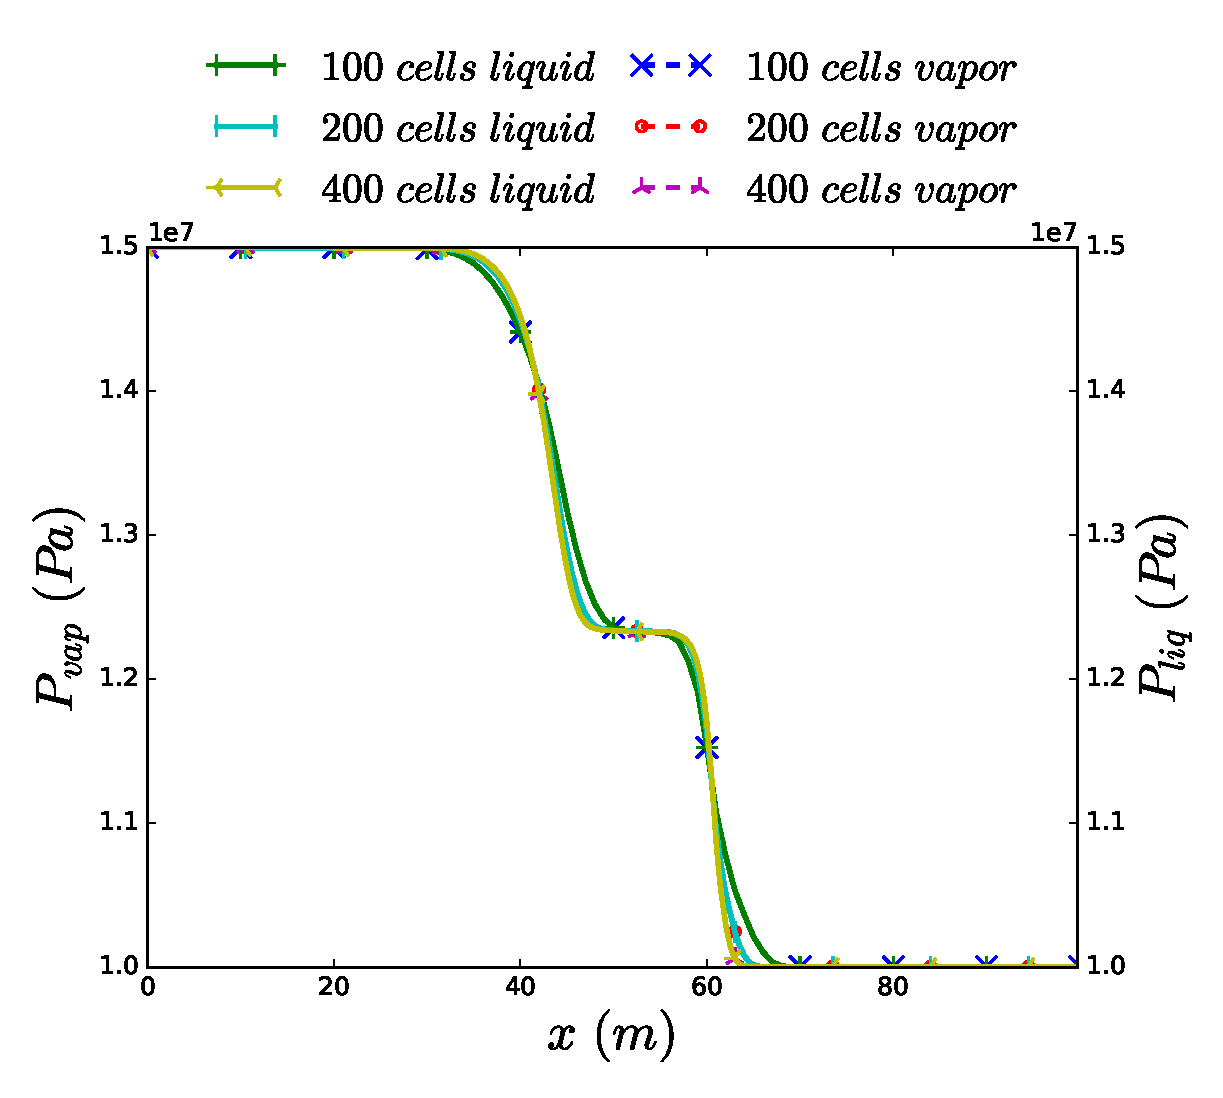
\includegraphics[width=\textwidth]{figures/two-phase-shock-tube-hem-pressure-plot.eps}                
                \caption{Pressure}
                \label{fig:2p-shock-tube-plots-press-hem-sa}
        \end{subfigure}%

        \begin{subfigure}[b]{0.49\textwidth}
                \centering
                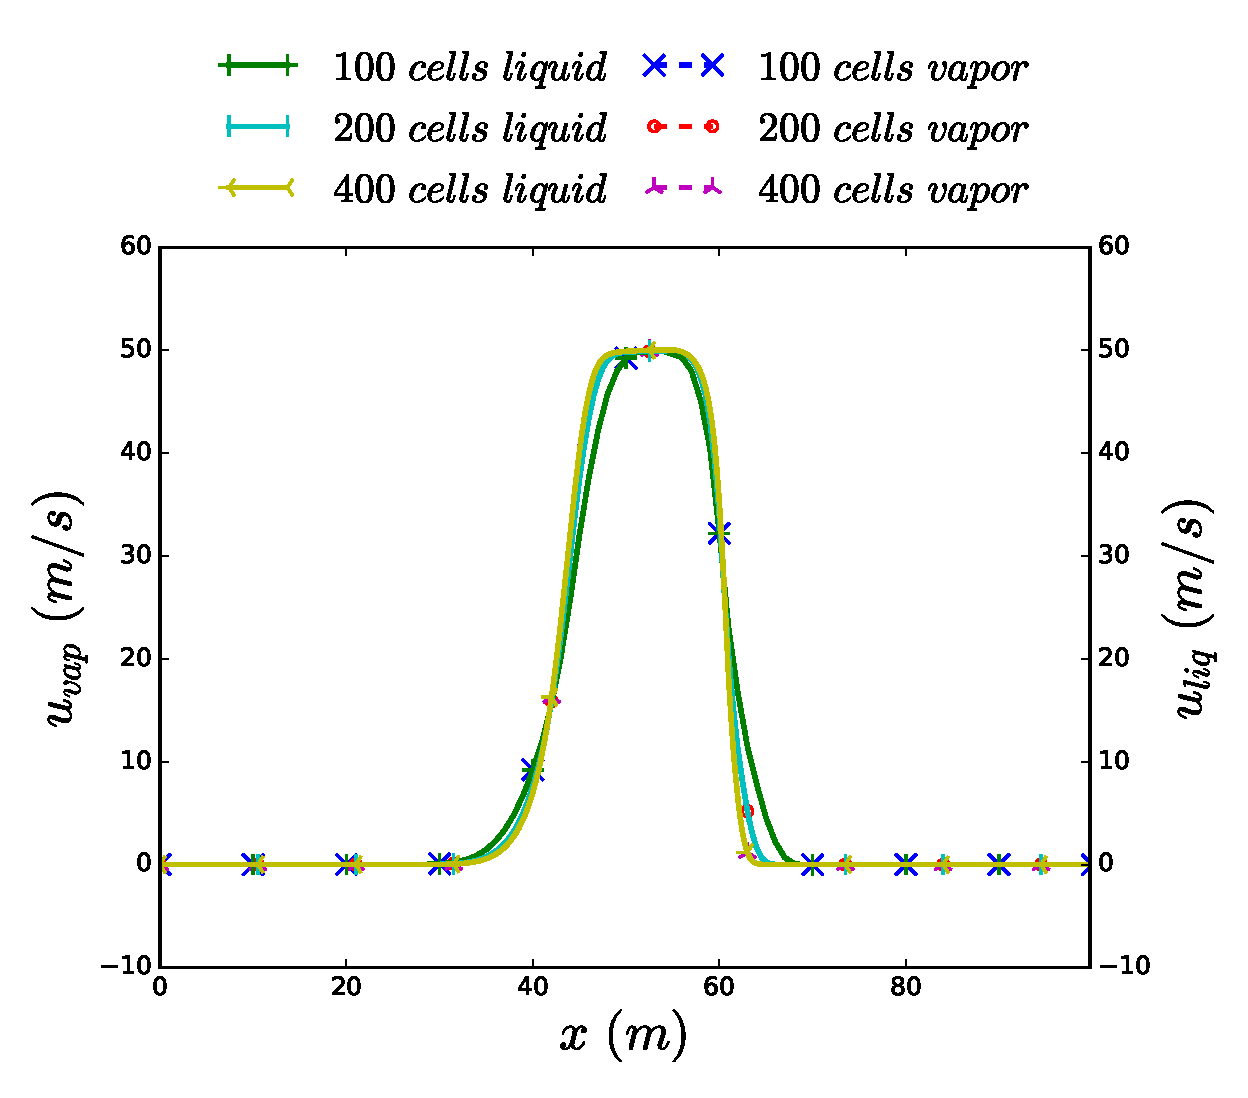
\includegraphics[width=\textwidth]{figures/two-phase-shock-tube-hem-velocity-plot.eps}              
                \caption{Velocity}
                \label{fig:2p-shock-tube-plots-velocity-hem-sa}
        \end{subfigure}        
        \begin{subfigure}[b]{0.49\textwidth}
                \centering
                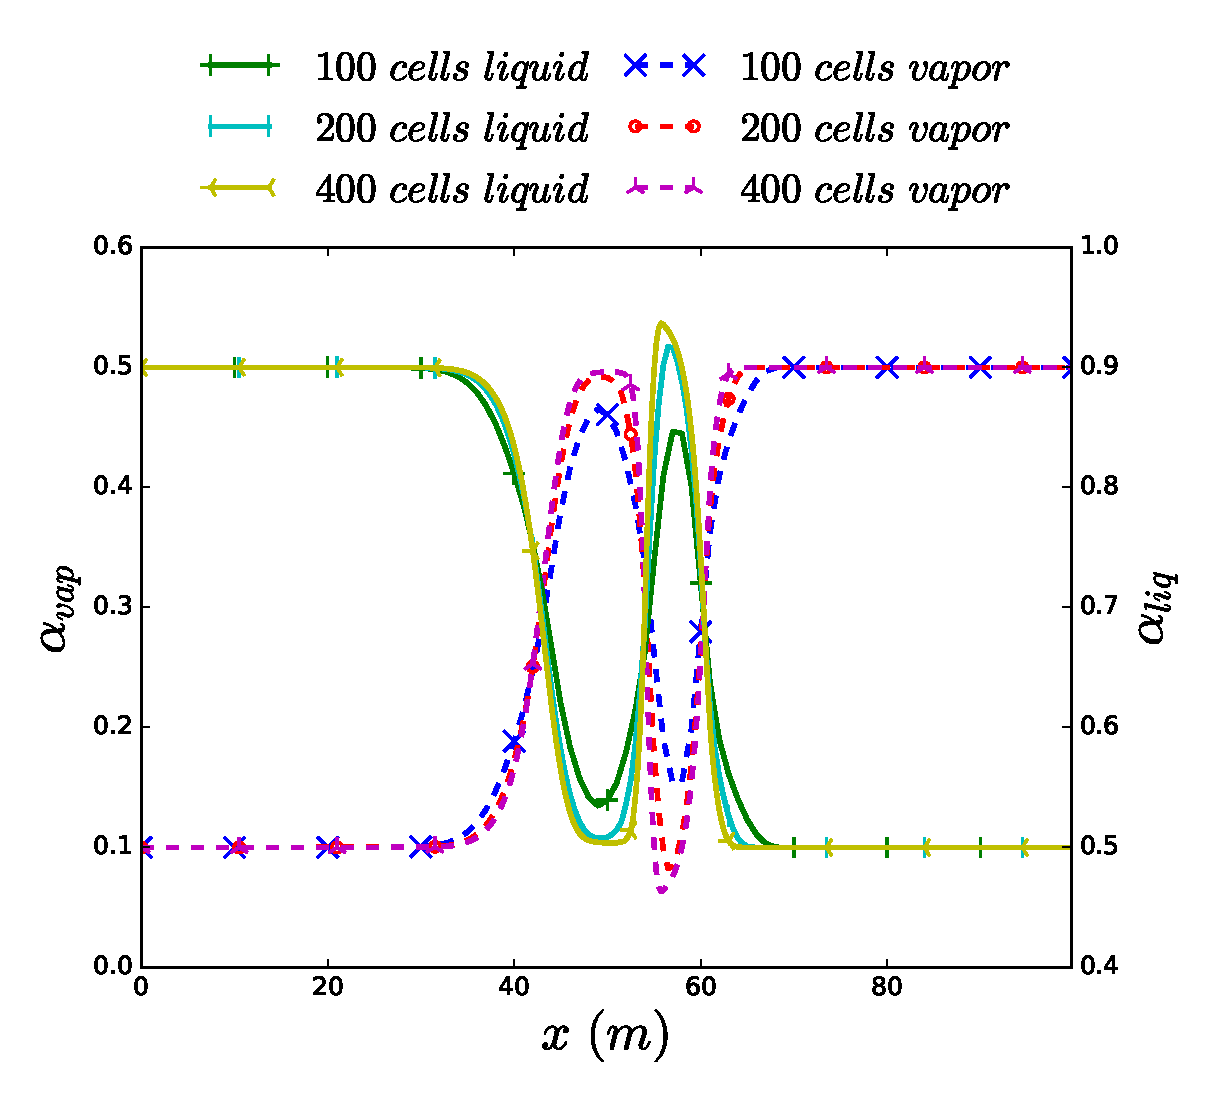
\includegraphics[width=\textwidth]{figures/two-phase-shock-tube-hem-vf-plot.eps}              
                \caption{Volume-fraction}
                \label{fig:2p-shock-tube-plots-vf-hem-sa}
        \end{subfigure}
        \vspace{-1 mm}        
        \caption{Numerical solutions of a two-phase flow shock tube at $t=8.1 \cdot 10^{-2} \ s$ for meshes with $100$, $200$ and $400$ cells.}\label{fig:2p-shock-tube-plots-hem-kapila}        
\end{figure}        
%
%The velocity and pressure profiles are given in \fig{fig:2p-shock-tube-plots-vel} and \fig{fig:2p-shock-tube-plots-press}, respectively, and show that the phasic velocity and phasic pressure are equal. 
%The numerical results presented in \fig{fig:2p-shock-tube-plots} show different flow behaviors between set (1) and set (2). 
The phasic pressures (\fig{fig:2p-shock-tube-plots-press-hem-sa}), velocities (\fig{fig:2p-shock-tube-plots-velocity-hem-sa}) and temperatures (\fig{fig:2p-shock-tube-plots-temp-hem-sa}) are equal as expected since a large interfacial area was used. The phasic density profiles in \fig{fig:2p-shock-tube-plots-rho-hem-sa} display a shock wave ($x \simeq$ 60 m) and a rarefaction wave ($x \simeq$ 20 m). The contact wave ($x \simeq$ 50 m) shows in the mixture density, $\rho_{m}$, profile that is defined as the sum over phasic densities weighted by the phasic volume fractions. The phasic volume fraction profiles plotted in \fig{fig:2p-shock-tube-plots-vf-hem-sa} display the three waves, i.e., shock, contact and rarefaction waves. Overall the numerical solutions do not display any instabilities in the vicinity of the shock wave and the contact wave. As the mesh gets refined the discontinuities are better resolved. Notably, going from 100 to 200 cells greatly improves the accuracy of the numerical solution. These results compare well to the ones obtained with the WAHA system code and showed in Fig. 8.2-1 (velocity and temperature) and Fig. 8.2-2 (pressure and volume fraction) of \cite{waha-manual}, and also to the ones obtained with the RELAP-5 system code presented in \cite{Sokolowski-Koszela}. The same dissipative behavior as in Fig. 8.2-1 of \cite{waha-manual} in the vicinity of the shock and the rarefaction waves is observed. 
%
%In set (2) that is Kapila-like, the phasic pressures and velocities are equal whereas the phasic temperatures are distinct since the interfacial heat transfer was set to zero. The same type of flow as in set (1) is observed but with different wave speed, with a shock wave (x $\simeq$ 80 m), a contact wave (x $\simeq$ 50 m) and a rarefaction wave (x $\simeq$ 20 m). Note that these results were not obtained with neither WAHA nor RELAP-7 to the best of our knowledge. This case illustrates the The pressure profile displays a small bump around x = 50 m that corresponds to the location of the contact wave. Small oscillations are also observed in the velocity profiles at the same location, i.e. the contact wave region.
%
%The numerical results presented in \fig{fig:2p-shock-tube-plots} show a shock wave (x $\simeq$ 75 m), a contact wave (x $\simeq$ 50 m) and a rarefaction wave (x $\simeq$ 20 m). Overall, the waves, notably the shock wave, get better resolved as the mesh is refined. The phasic pressure (\fig{fig:2p-shock-tube-plots-press}) and velocity (\fig{fig:2p-shock-tube-plots-vel}) profiles are equal as expected since large relaxation coefficients were used, whereas the phasic temperature (\fig{fig:2p-shock-tube-plots-temp}) are distinct. The pressure profile displays a small bump around x = 50 m that corresponds to the location of the contact wave. Small oscillations are also observed in the velocity profiles at the same location, i.e. the contact wave region. 
%The numerical solutions obtained with RELAP-5 and WAHA in Section 2.3 of \cite{Sokolowski-Koszela} for the same two-phase shock tube show different results as the two codes imply almost immediate mass, momentum and energy inter-phase transfer which causes the phasic velocities and temperatures to be nearly identical. In the present setup used to obtain the numerical solutions with RELAP-7, only mechanical equilibrium (same velocity and pressure) is achieved by using large relaxation coefficients $\mu_P$ and $\lambda_u$.
%%
%\begin{figure}[H]
%        \vspace{-1 mm}
%        \centering
%        \begin{subfigure}[b]{0.49\textwidth}
%                \centering
%                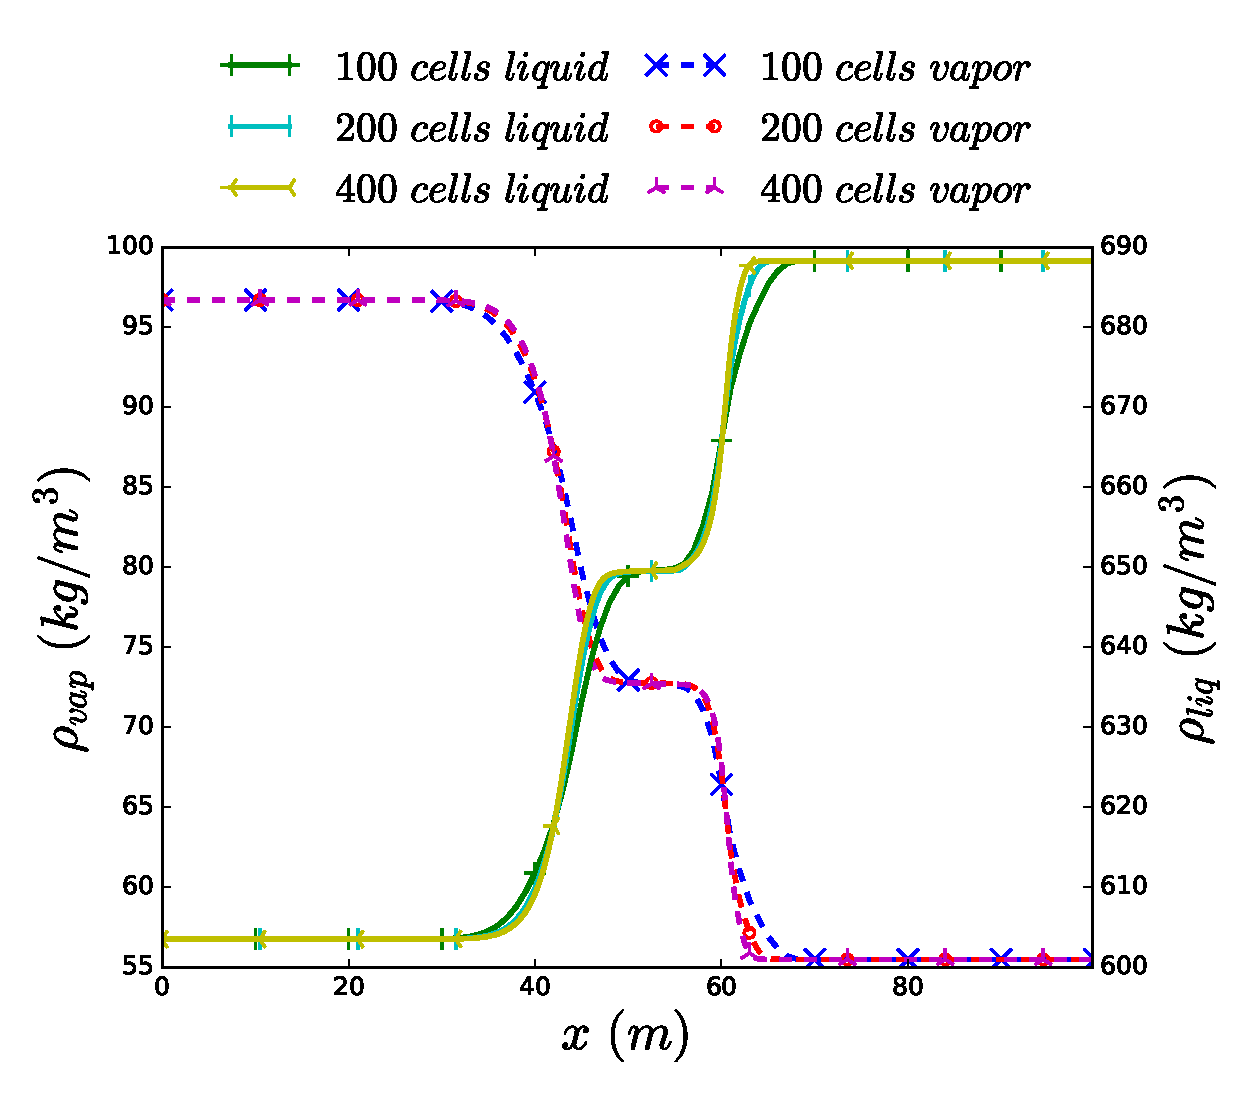
\includegraphics[width=\textwidth]{figures/two-phase-shock-tube-hem-density-plot.eps}                
%                \caption{Density, set (2)}
%                \label{fig:2p-shock-tube-plots-vel-hem-hem-sa}
%        \end{subfigure}%
%        \begin{subfigure}[b]{0.49\textwidth}
%                \centering
%                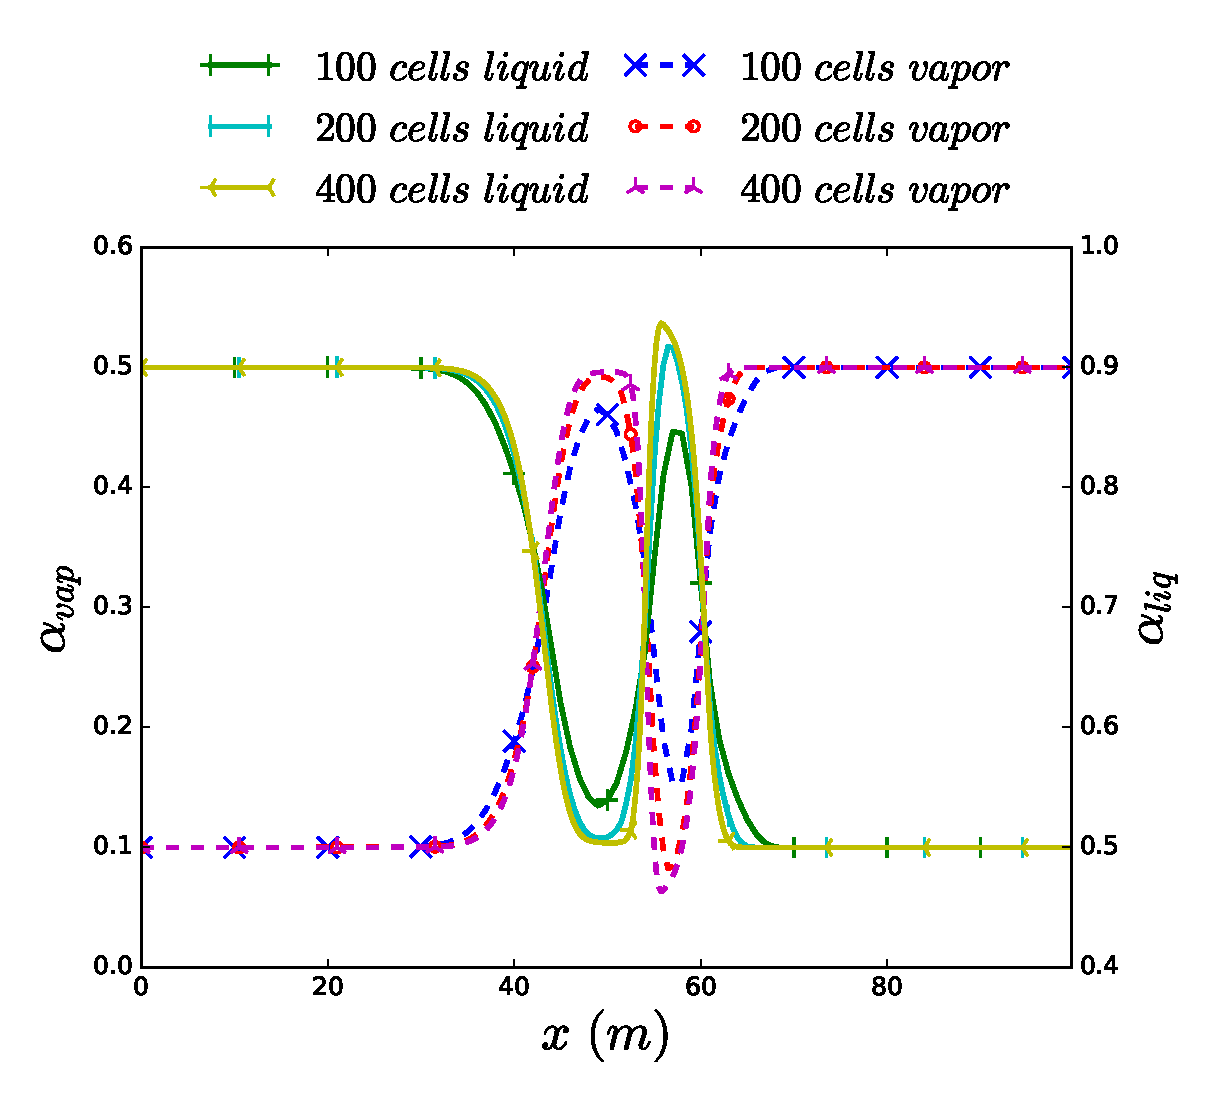
\includegraphics[width=\textwidth]{figures/two-phase-shock-tube-hem-vf-plot.eps}              
%                \caption{Volume-fraction, set (2)}
%                \label{fig:2p-shock-tube-plots-dens-hem-hem-sa}
%        \end{subfigure}
%        \vspace{-1 mm}
%        
%        \centering
%        \begin{subfigure}[b]{0.49\textwidth}
%                \centering
%                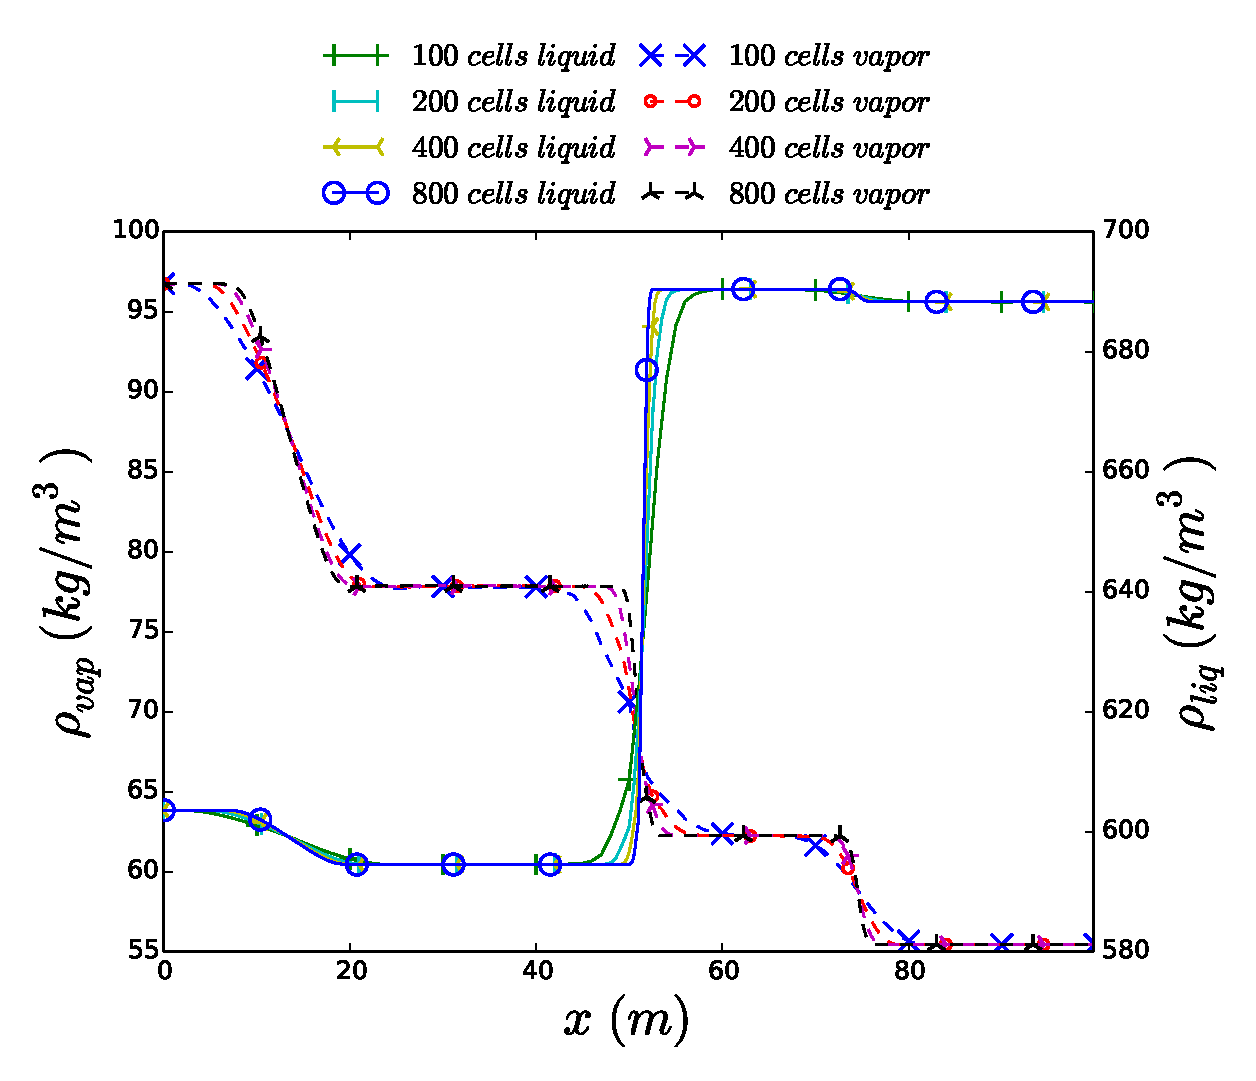
\includegraphics[width=\textwidth]{figures/two-phase-shock-tube-density-plot.eps}                
%                \caption{Density, set (1)}
%                \label{fig:2p-shock-tube-plots-vel-hem-kapila-sa}
%        \end{subfigure}%
%        \begin{subfigure}[b]{0.49\textwidth}
%                \centering
%                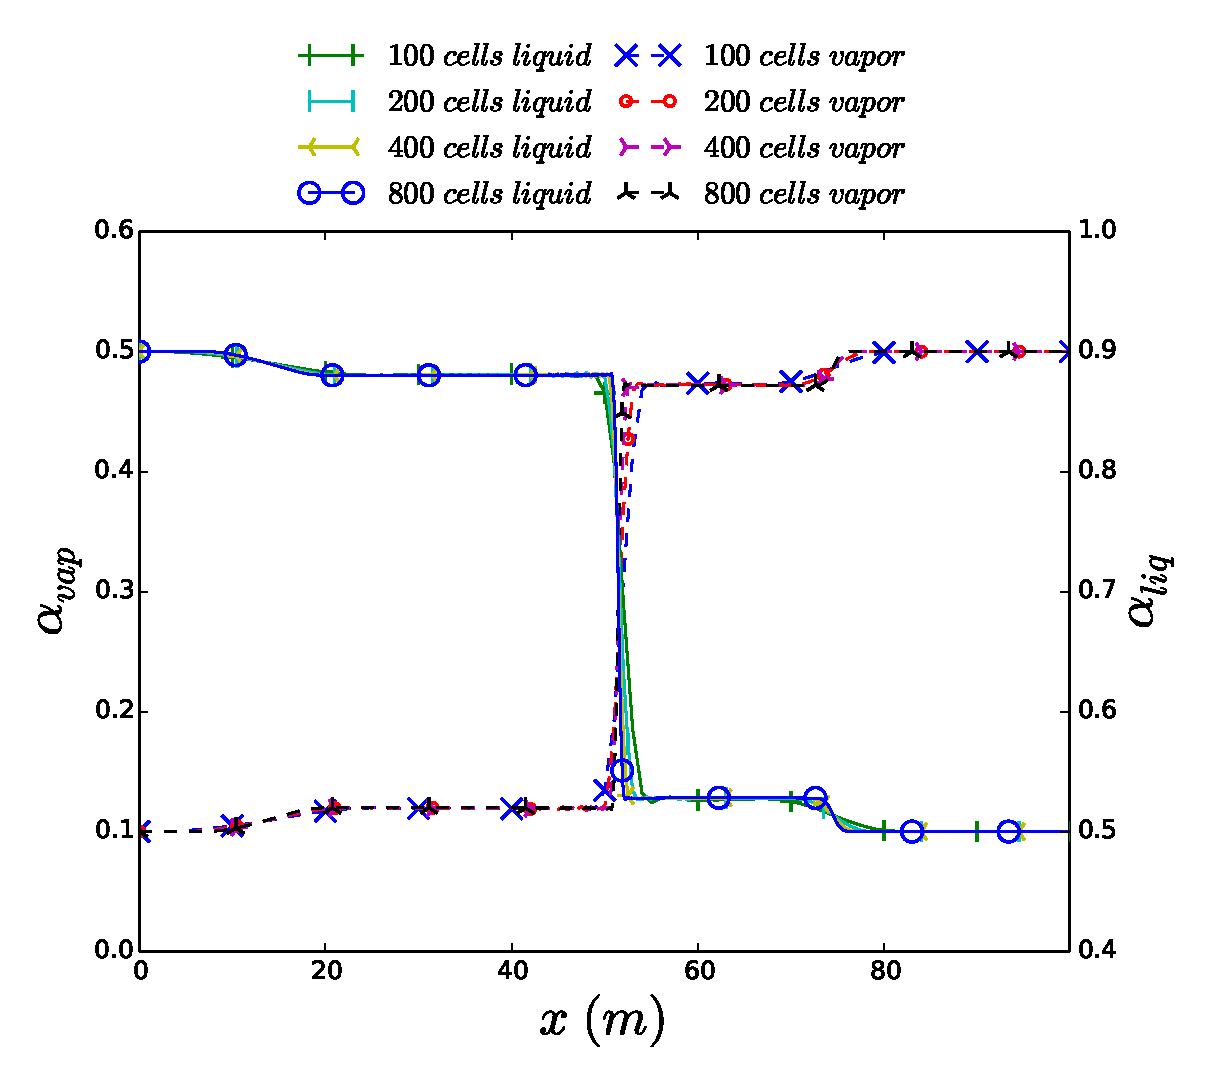
\includegraphics[width=\textwidth]{figures/two-phase-shock-tube-vf-plot.eps}              
%                \caption{Volume-fraction, set (1)}
%                \label{fig:2p-shock-tube-plots-dens-hem-kapila-sa}
%        \end{subfigure}
%        \vspace{-1 mm}        
%        \caption{Numerical solutions of a two-phase flow shock tube at $t=8.1 \cdot 10^{-2} \ s$ for mesh with $100$, $200$ and $400$ cells.}\label{fig:2p-shock-tube-plots-hem-kapila-sa}        
%\end{figure}        
%%
%%---------------------------------------------------------------------------------------------------
%\subsection{Single-phase water-hammer} \label{sec:single-num-res}
%%---------------------------------------------------------------------------------------------------
%%
%A single-phase water hammer consists of a liquid phase flowing in a straight 1-D pipe of length $L=10 \ m$ with initial uniform pressure ($P = 7$ MPa), velocity ($u = -12$ $m/s$) and temperature ($T = 453$ K). At $t=0$ s, the two extremities of the 1-D pipe are closed by solid walls which causes sharp compression (shock) and sharp rarefaction waves to appear at the left and right extremities, respectively. The two waves initially propagate towards the middle of the pipe and are reflected on the opposite wall after crossing each other near the middle of the pipe. Numerical results of the velocity, density and pressure profiles are given in \fig{fig:single-phase-vel}, ~\ref{fig:single-phase-density} and ~\ref{fig:single-phase-press}, respectively.\, for three different times $t=8.7 \times 10^{-4}, \, 6.8 \times 10^{-3} \text{ and } 10^{-3}$ s. The viscosity coefficients are plotted in \fig{fig:single-phase-visc} at time $t = 8.7 \times 10^{-4}$ s only.
%%
%\begin{figure}[H]
%        \centering
%        \begin{subfigure}[b]{0.5\textwidth}
%                \centering
%                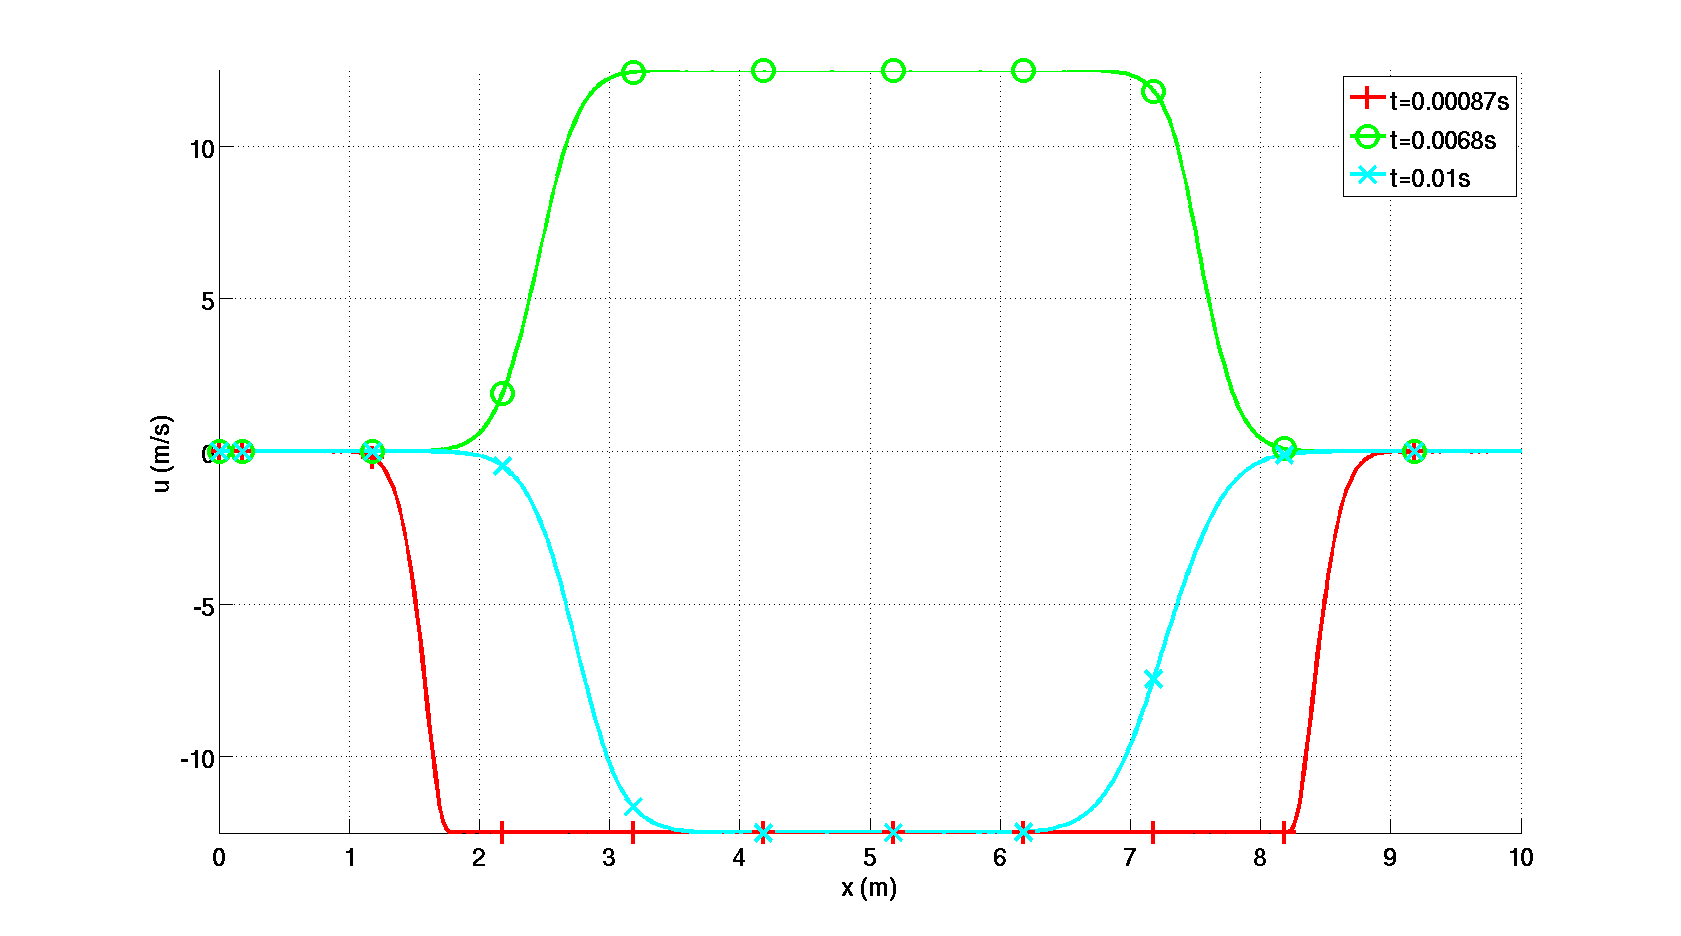
\includegraphics[width=\textwidth]{figures/Plot_velocity_single_phase.png}
%                \caption{Velocity}
%                \label{fig:single-phase-vel}
%        \end{subfigure}%
%        \begin{subfigure}[b]{0.5\textwidth}
%                \centering
%                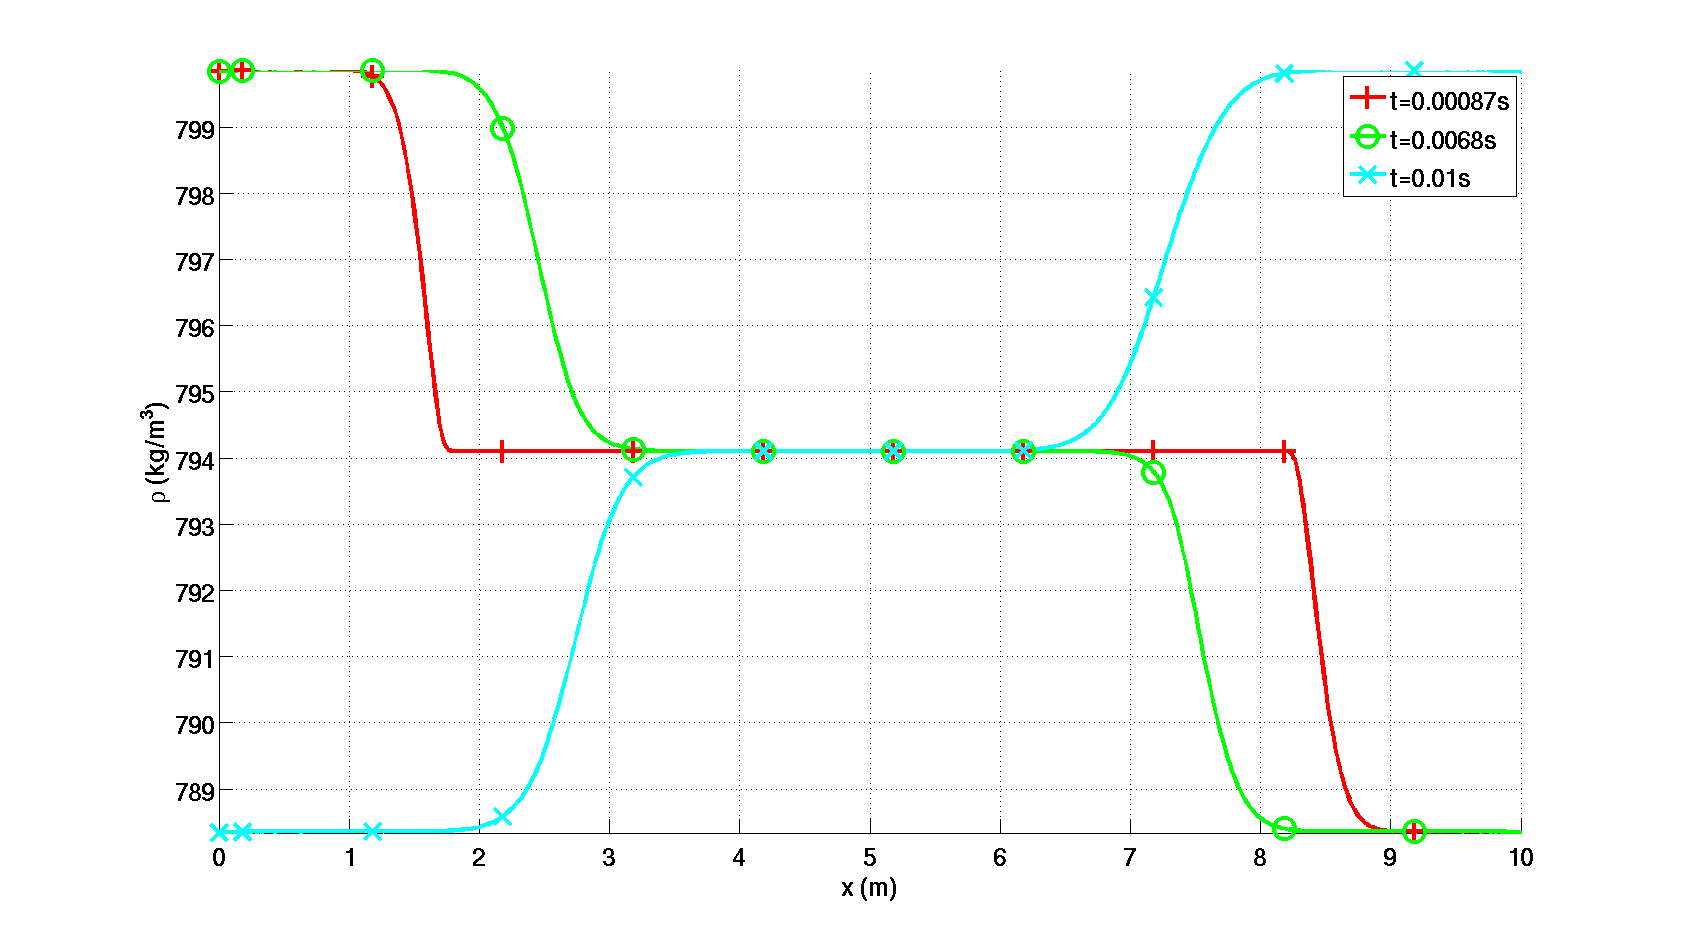
\includegraphics[width=\textwidth]{figures/Plot_density_single_phase.png}
%                \caption{Density}
%                \label{fig:single-phase-density}
%        \end{subfigure}
%        
%        \begin{subfigure}[b]{0.495\textwidth}
%                \centering
%                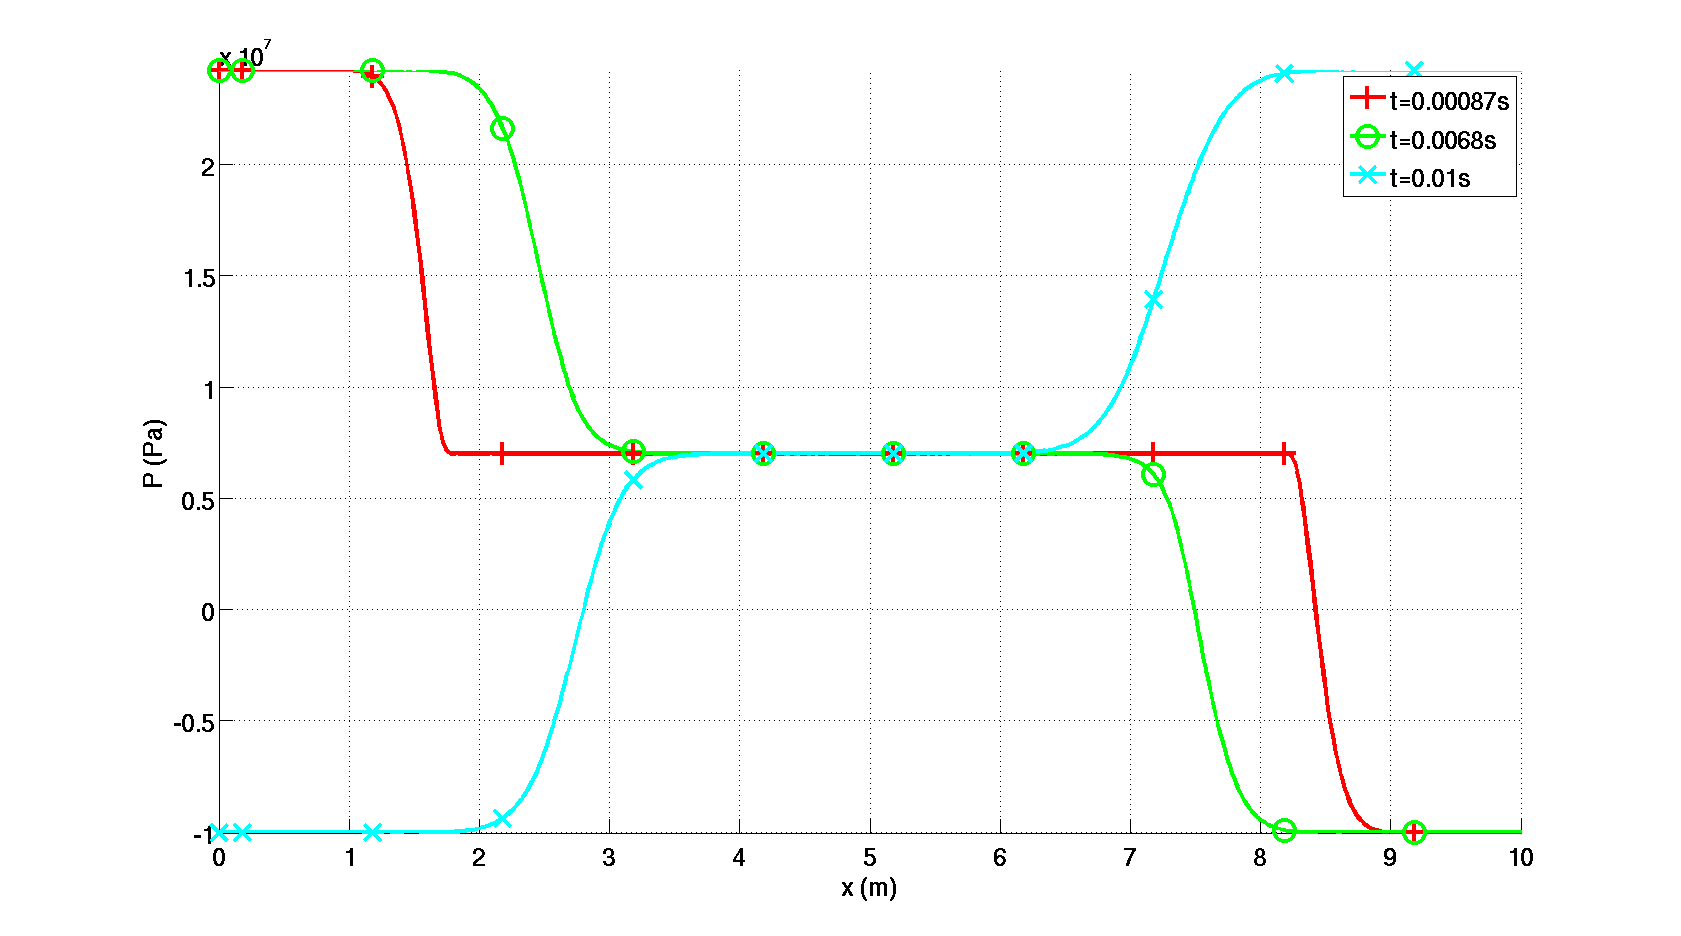
\includegraphics[width=\textwidth]{figures/Plot_pressure_single_phase.png}
%                \caption{Pressure}
%                \label{fig:single-phase-press}
%        \end{subfigure}        
%        \begin{subfigure}[b]{0.495\textwidth}
%                \centering
%                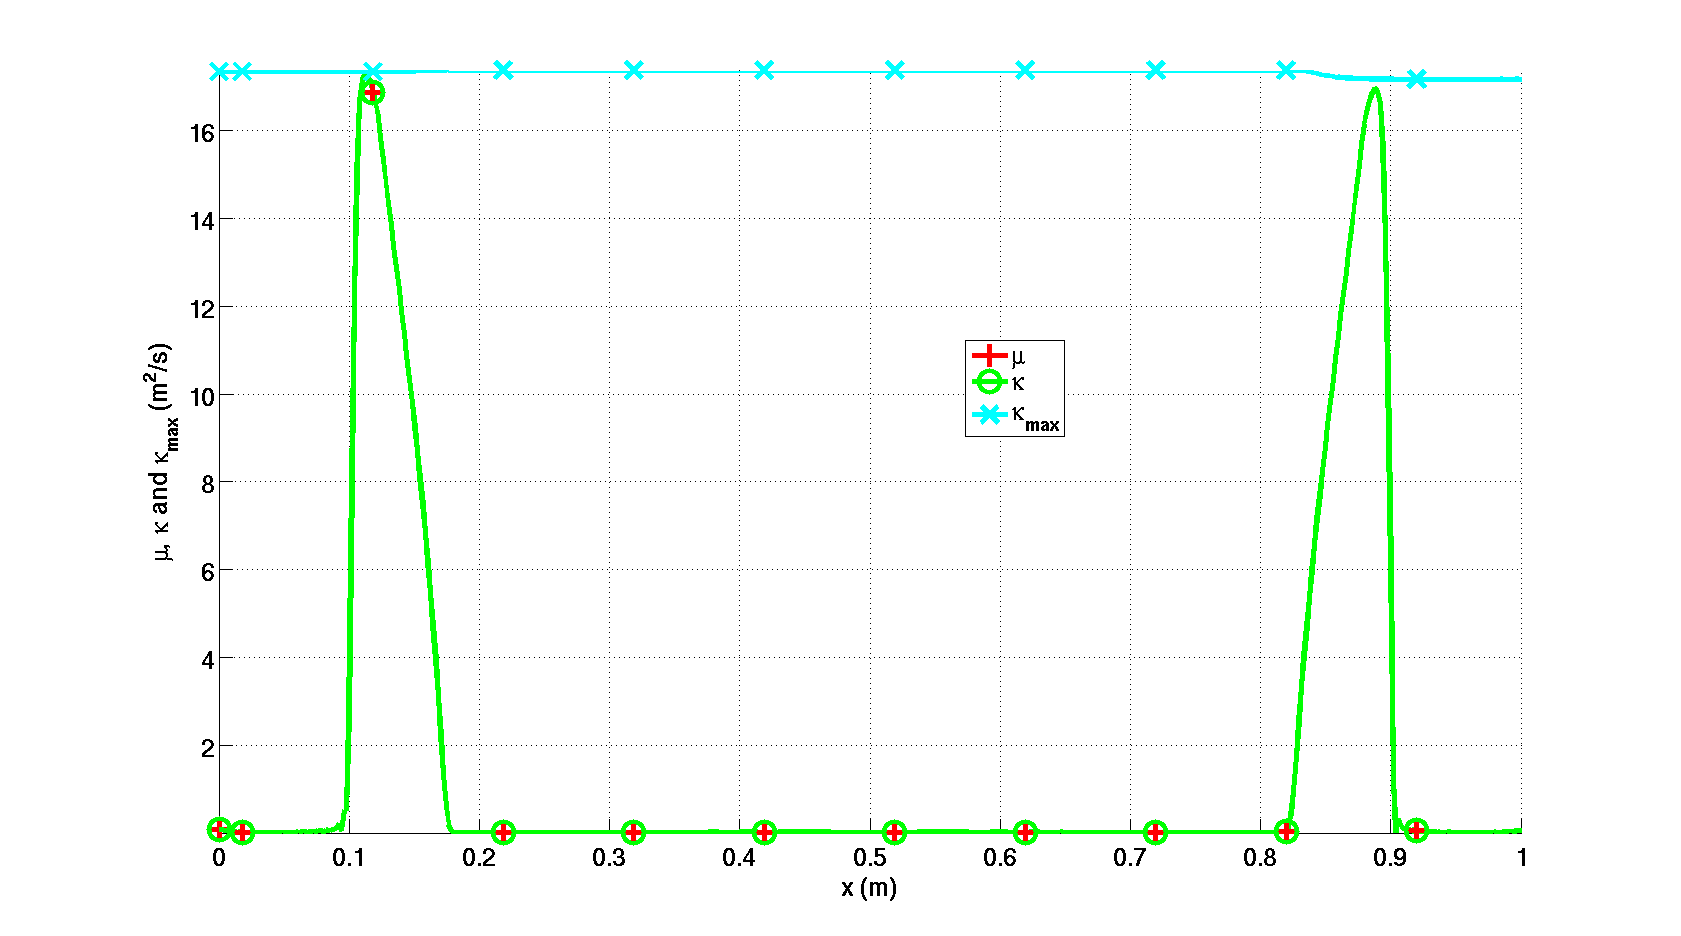
\includegraphics[width=\textwidth]{figures/Plot_viscosity_single_phase.png}
%                \caption{Viscosity coefficients}
%                \label{fig:single-phase-visc}
%        \end{subfigure}
%        \caption{Numerical solutions of a water hammer at times $t=8.7 \times 10^{-4}, \, 6.8 \times 10^{-3} \text{ and } 10^{-3}$ s (the viscosity coefficients are only shown at time $t=8.7 \times 10^{-4}$ s).}\label{fig:single-phase}
%\end{figure}
%%
%In \fig{fig:single-phase}, the numerical solution does not display any oscillations or any spurious instabilities due to the numerics. The viscosity coefficients $\kappa$ and $\mu$ only saturate to the first-order viscosity coefficients, $\kappa_{max}$, around $x=0.1$ m and $x=0.9$ m which match the positions of the wave fronts at $t=8.7 \times 10^{-4}$. It is also noted that the accuracy of the compression (shock) wave decreases over time: the numerical dissipation comes from the temporal integrator (time step size) and the spatial discretize element size. The accuracy of the numerical solution could be improved over time by using a finer grid with smaller time steps or a higher-order temporal integrator. In \fig{fig:single-phase-press}, the pressure temporarily becomes negative as the liquid phase cannot vaporize in the model used. Such negative pressure variations are allowed by the stiffened gas equation of state.
%
%%---------------------------------------------------------------------------------------------------
%\subsubsection{Two-phase flow water hammer} \label{sec:two-num-res}
%%---------------------------------------------------------------------------------------------------
%
%The two-phase water hammer is identical to the single-phase water hammer described in \sct{sec:two-num-res}: the liquid and vapor phases have the same initial conditions and the liquid volume fraction is initially set to $0.5$. The two phases are interact through the pressure and velocity relaxation terms (see \eqt{eq:sem-eq}) that are functions of the relaxation coefficients, $\mu_P$ and $\lambda_u$, computed with $A_{int} = 10^3$ $m^{-1}$ so that the two phases nearly achieve pressure and velocity equilibrium at all times. Plots of the velocity, the density, the pressure and the viscosity coefficients are given in \fig{fig:liquid-phase} and \ref{fig:vapor-phase} for the liquid and gas phases, respectively.
%%
%\begin{figure}[H]
%        \centering
%        \begin{subfigure}[b]{0.5\textwidth}
%                \centering
%                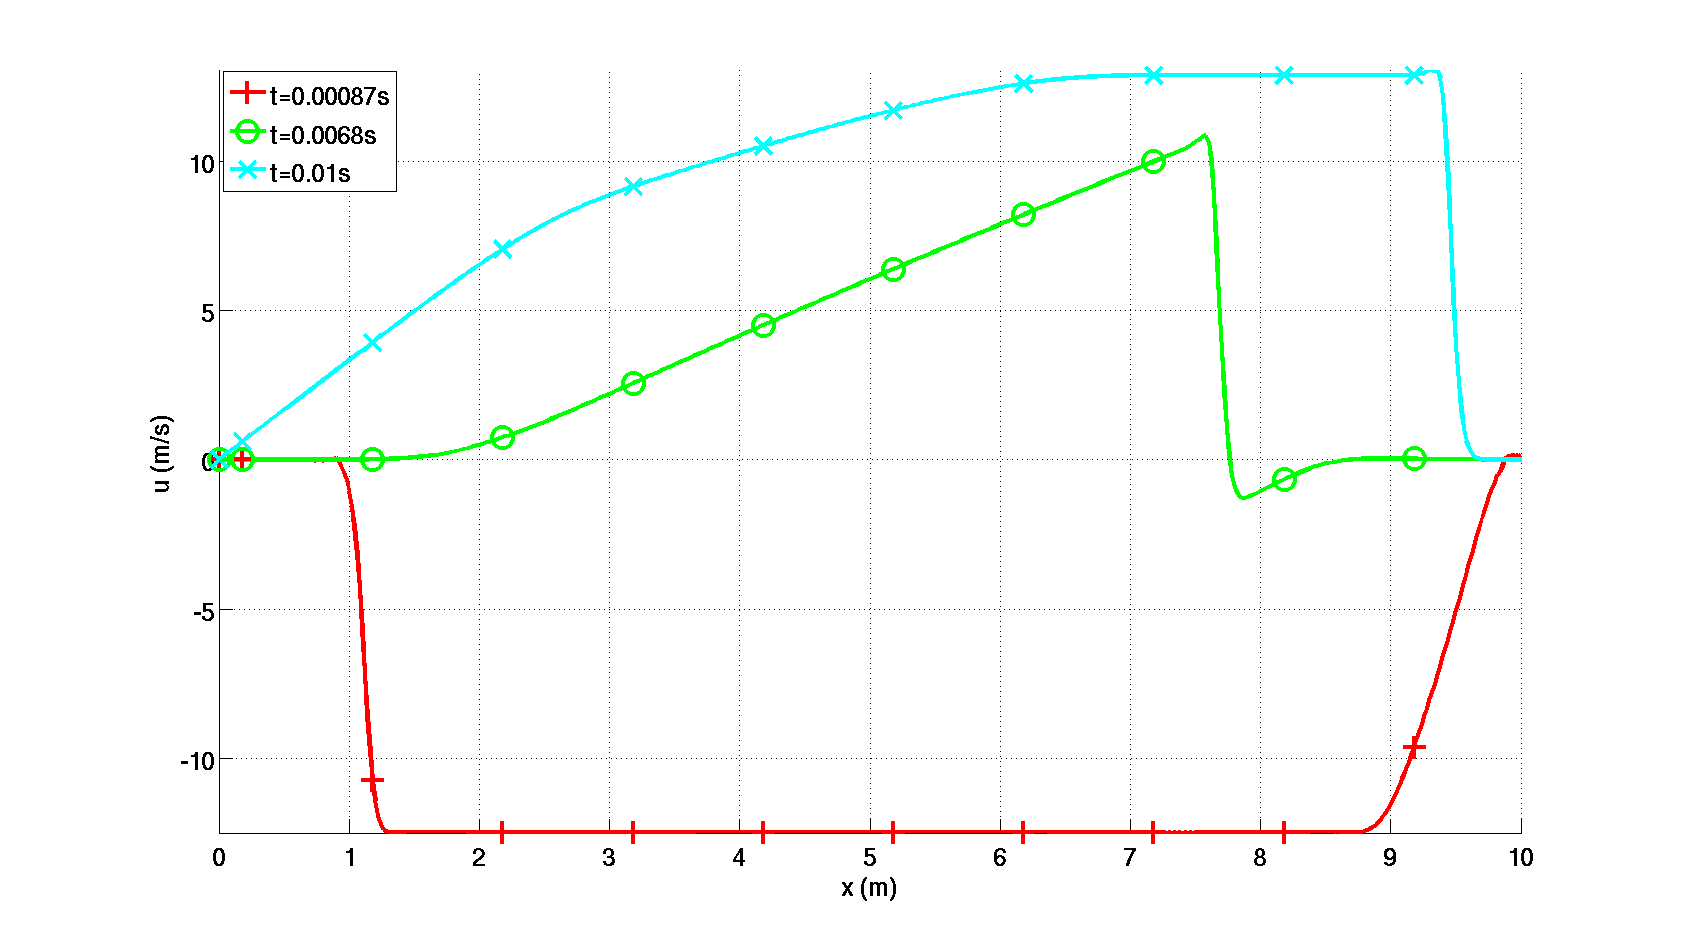
\includegraphics[width=\textwidth]{figures/Plot_velocity_liquid_phase.png}
%                \caption{Liquid velocity}
%                \label{fig:liq-phase-vel}
%        \end{subfigure}%
%        \begin{subfigure}[b]{0.5\textwidth}
%                \centering
%                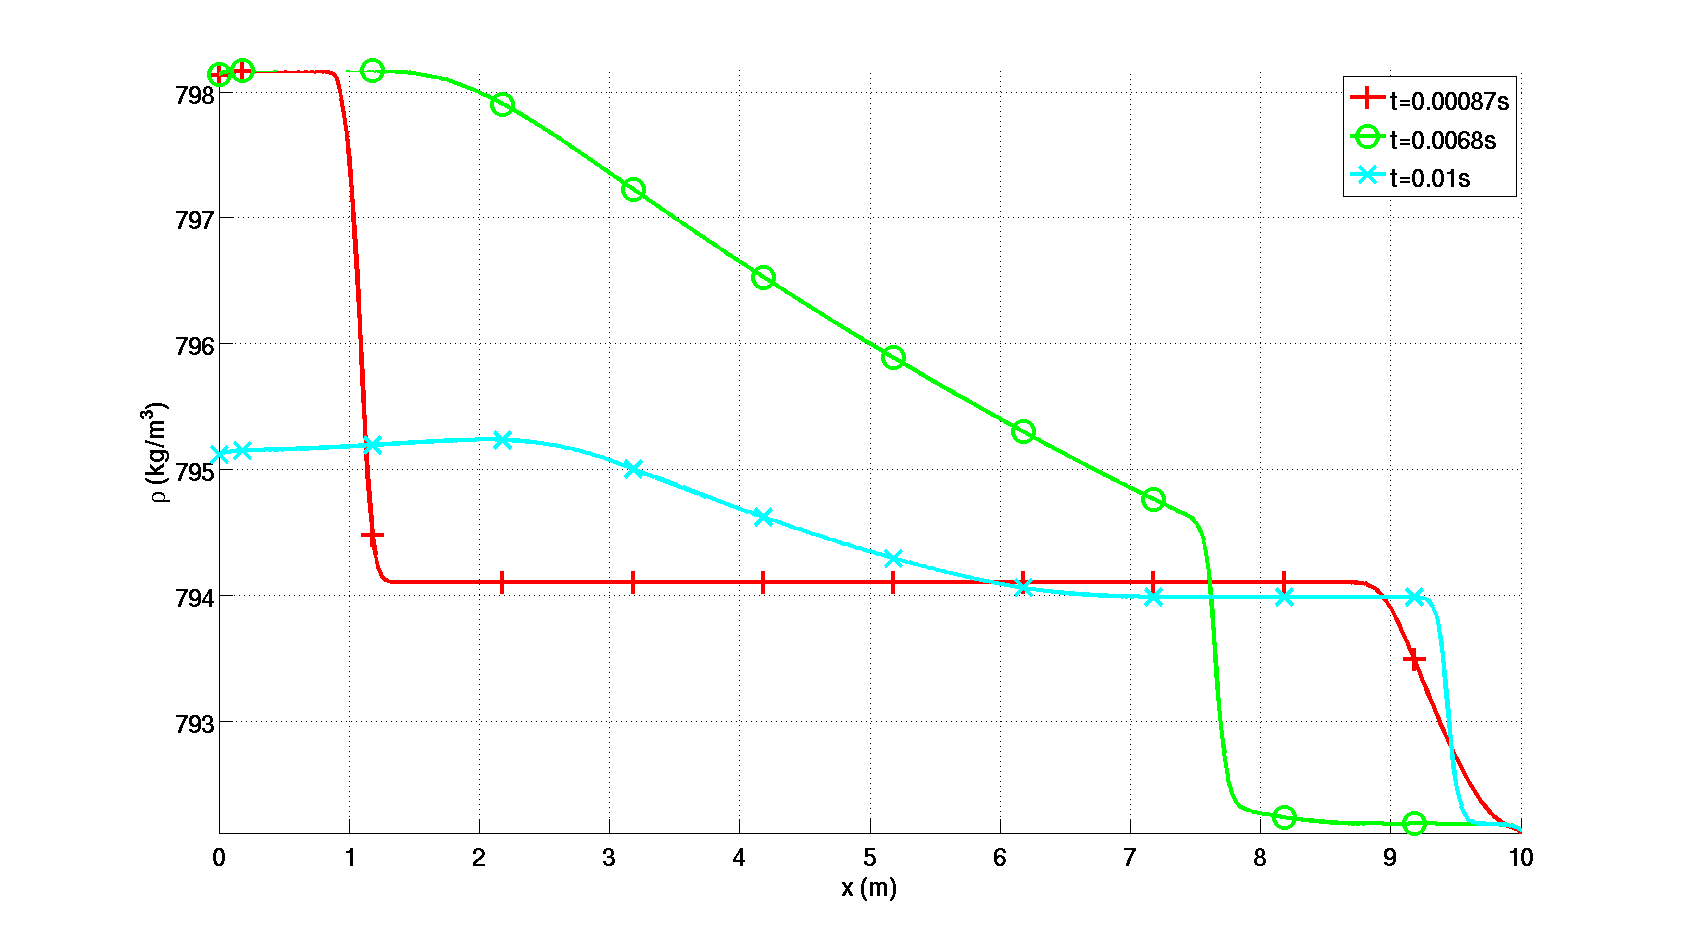
\includegraphics[width=\textwidth]{figures/Plot_density_liquid_phase.png}
%                \caption{Liquid density}
%                \label{fig:liq-phase-density}
%        \end{subfigure}
%        
%        \begin{subfigure}[b]{0.495\textwidth}
%                \centering
%                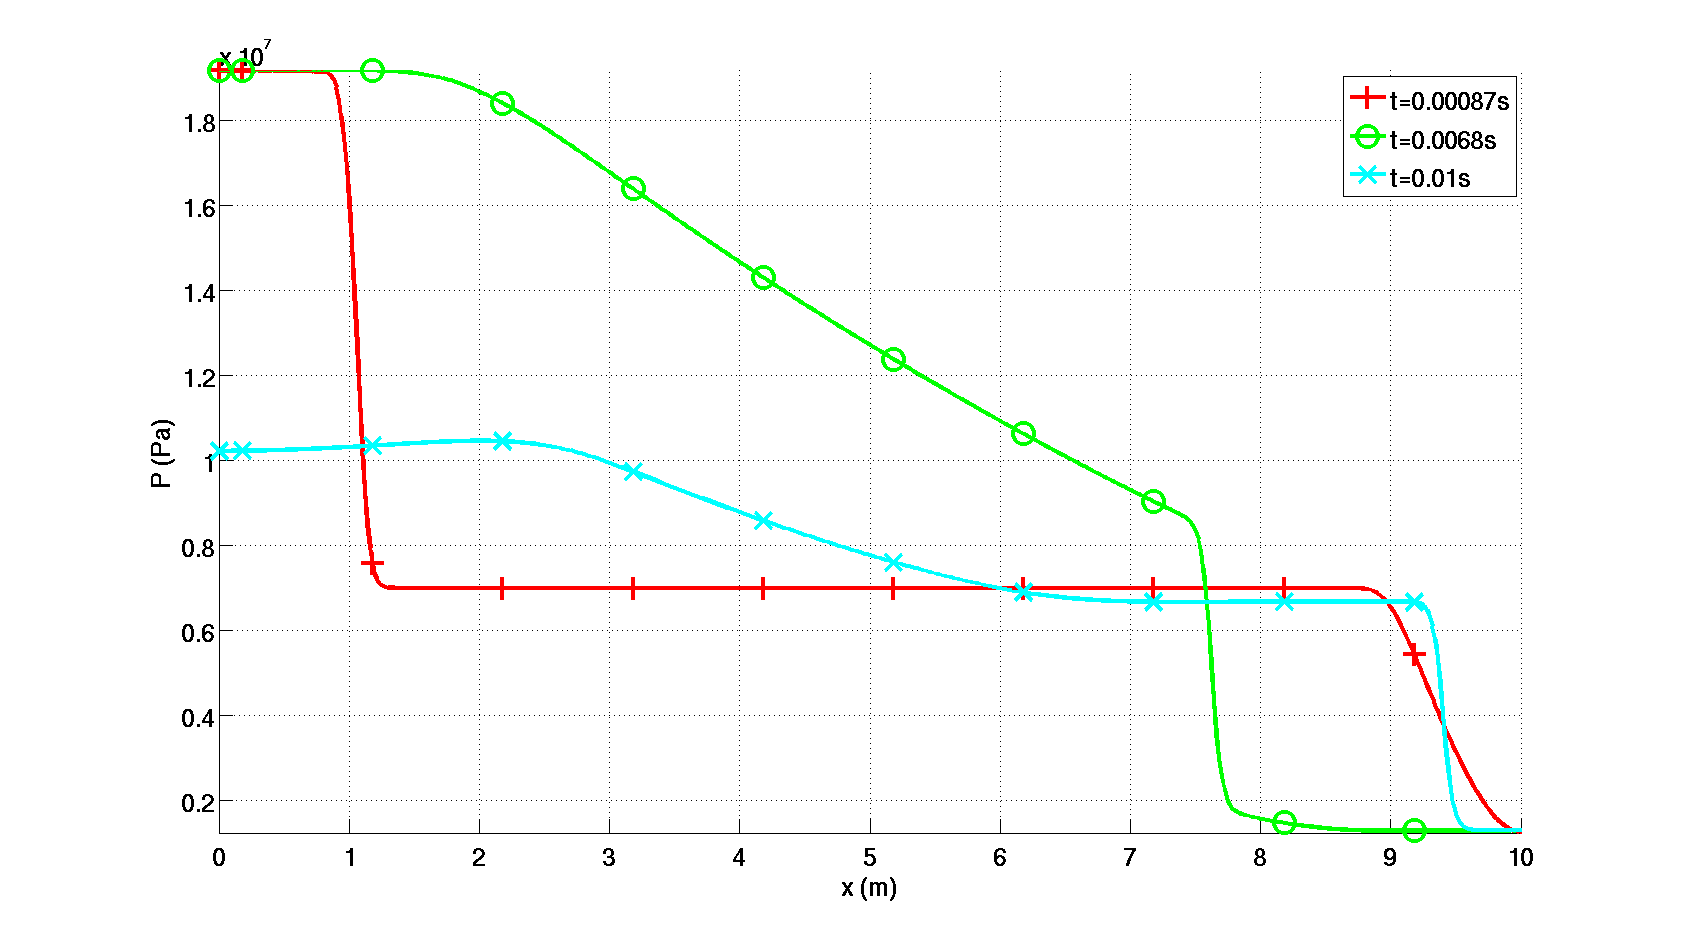
\includegraphics[width=\textwidth]{figures/Plot_pressure_liquid_phase.png}
%                \caption{Liquid pressure}
%                \label{fig:liq-phase-press}
%        \end{subfigure}        
%        \begin{subfigure}[b]{0.495\textwidth}
%                \centering
%                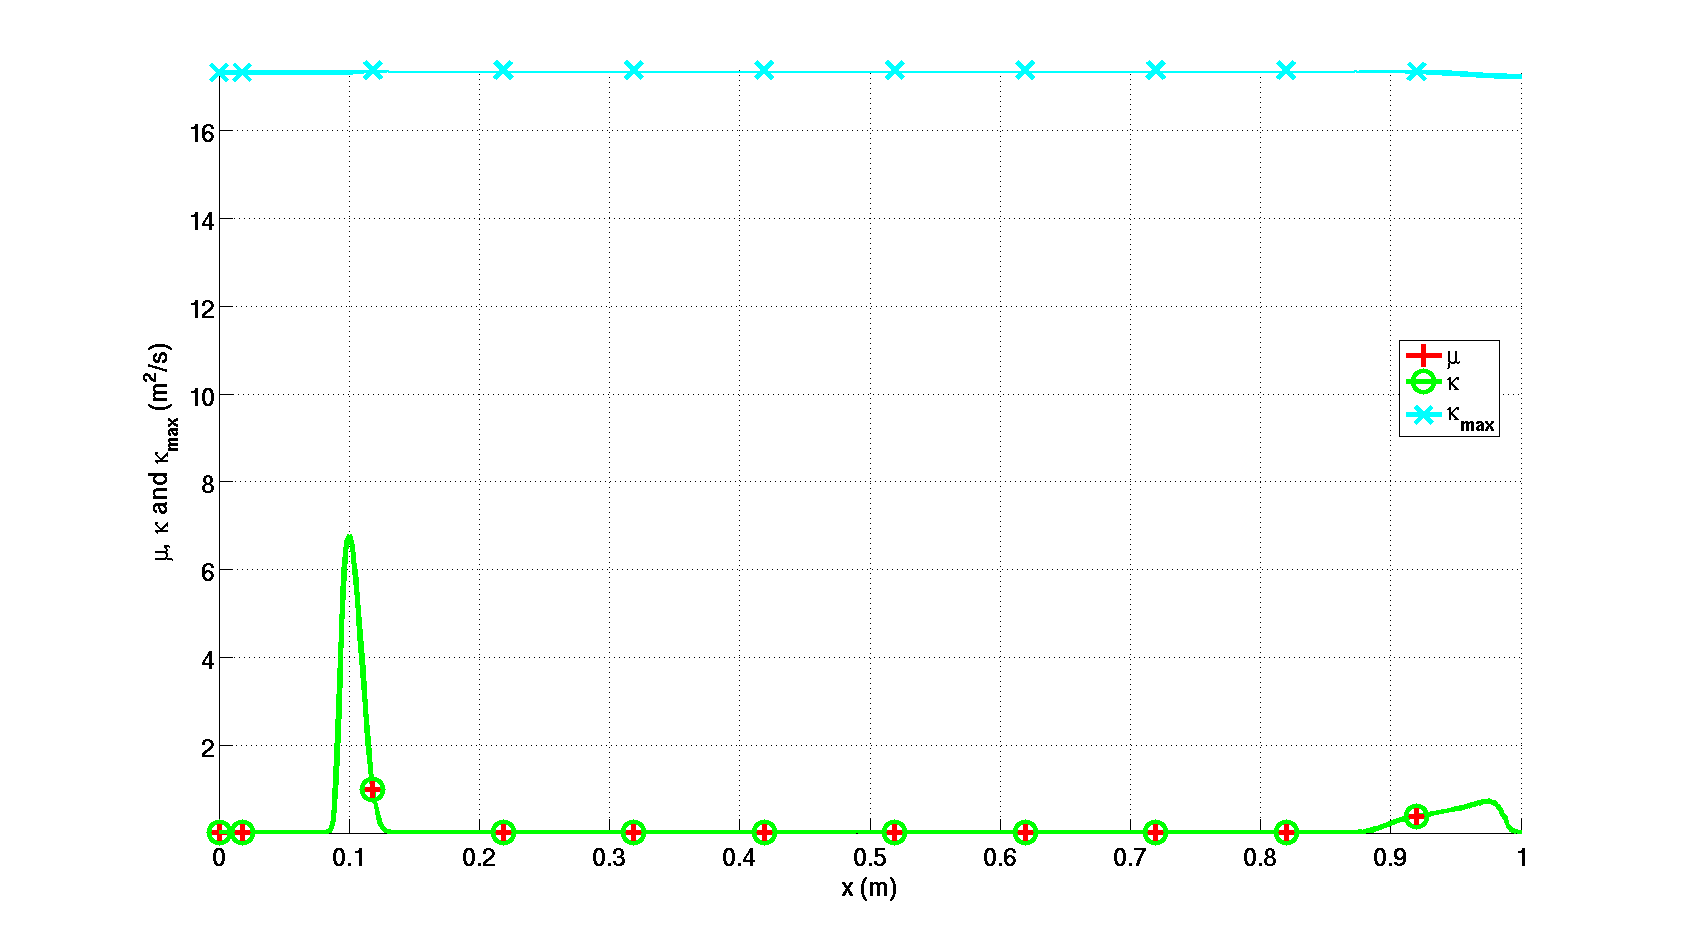
\includegraphics[width=\textwidth]{figures/Plot_viscosity_liquid_phase.png}
%                \caption{Liquid viscosity coefficients}
%                \label{ffig:liq-phase-visc}
%        \end{subfigure}
%        \caption{Numerical solutions for the liquid phase of a two-phase water hammer at times $t=8.7 \times 10^{-4}, \, 6.8 \times 10^{-3} \text{ and } 10^{-3}$ s (the viscosity coefficients are only shown at time $t=8.7 \times 10^{-4}$ s).}\label{fig:liquid-phase}
%\end{figure}
%%
%%
%\begin{figure}[H]
%        \centering
%        \begin{subfigure}[b]{0.5\textwidth}
%                \centering
%                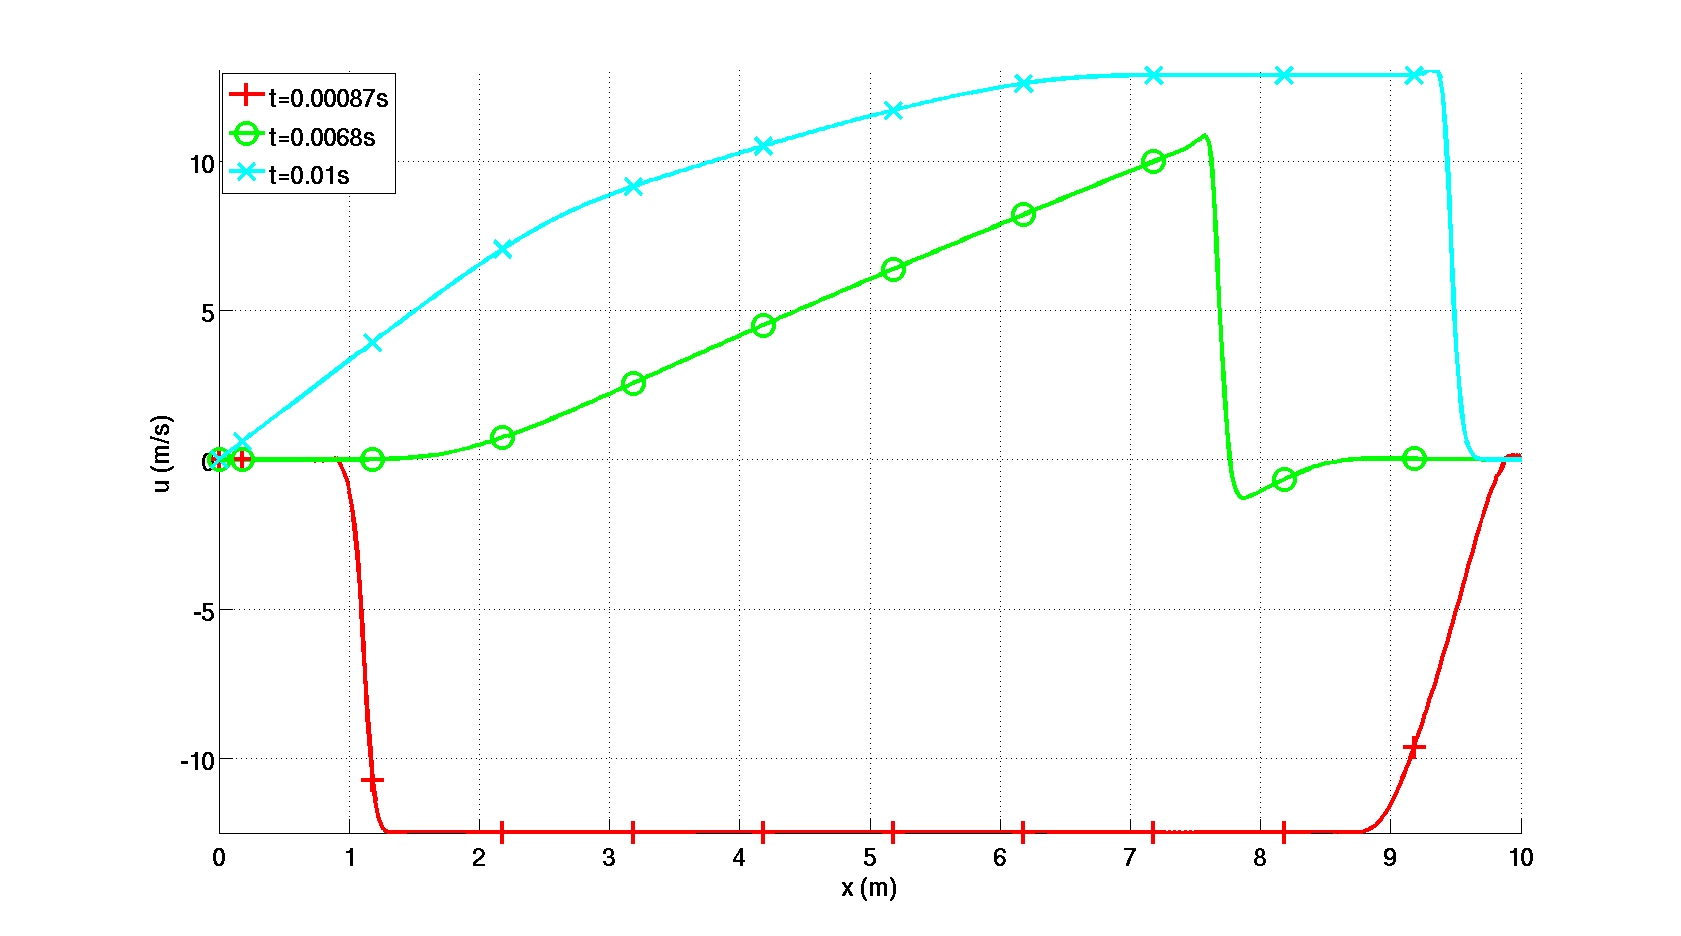
\includegraphics[width=\textwidth]{figures/Plot_velocity_gas_phase.png}
%                \caption{Gas velocity}
%                \label{fig:vap-phase-vel}
%        \end{subfigure}%
%        \begin{subfigure}[b]{0.5\textwidth}
%                \centering
%                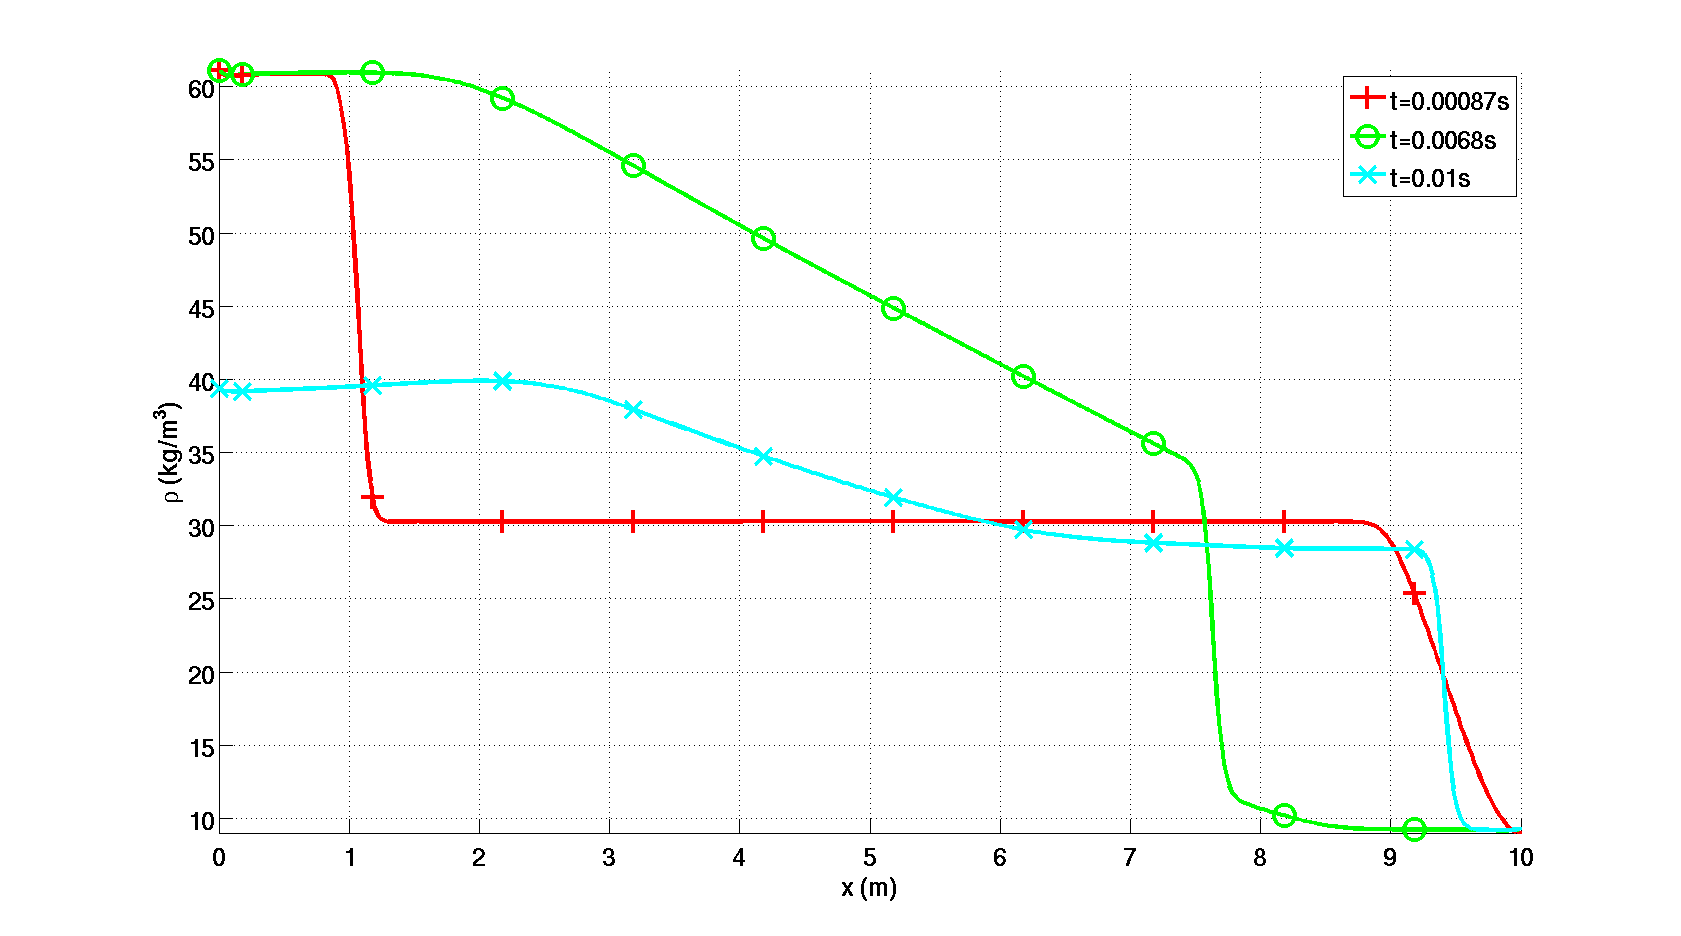
\includegraphics[width=\textwidth]{figures/Plot_density_gas_phase.png}
%                \caption{Gas density}
%                \label{fig:vap-phase-density}
%        \end{subfigure}
%        
%        \begin{subfigure}[b]{0.495\textwidth}
%                \centering
%                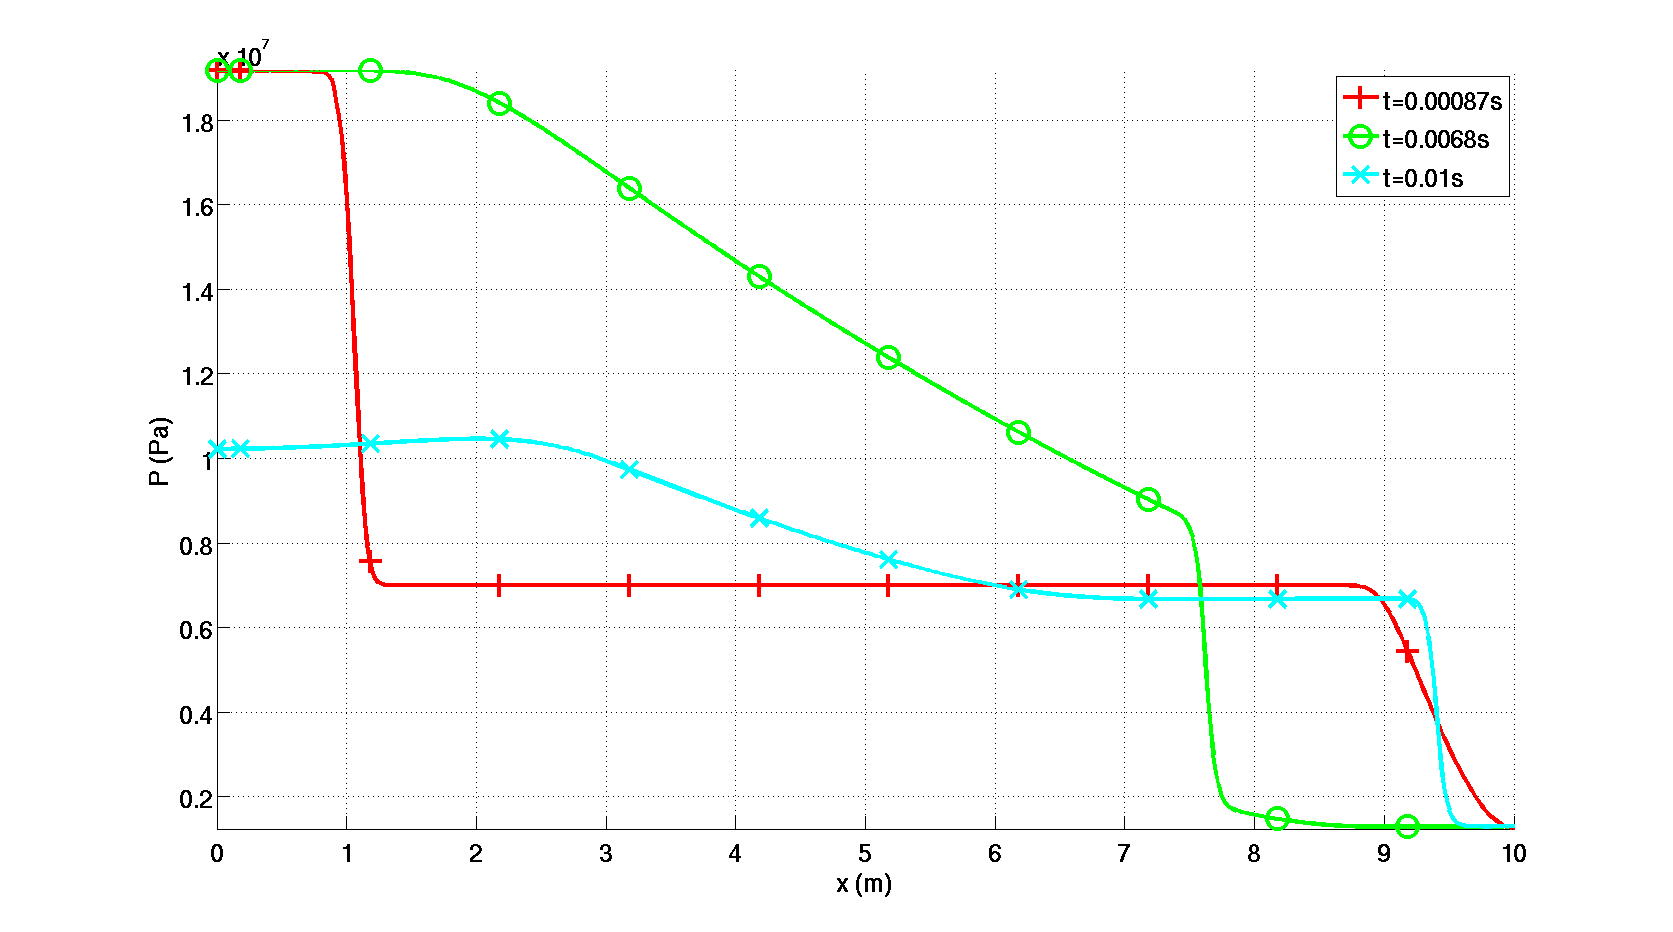
\includegraphics[width=\textwidth]{figures/Plot_pressure_gas_phase.png}
%                \caption{Gas pressure}
%                \label{fig:vap-phase-press}
%        \end{subfigure}        
%        \begin{subfigure}[b]{0.495\textwidth}
%                \centering
%                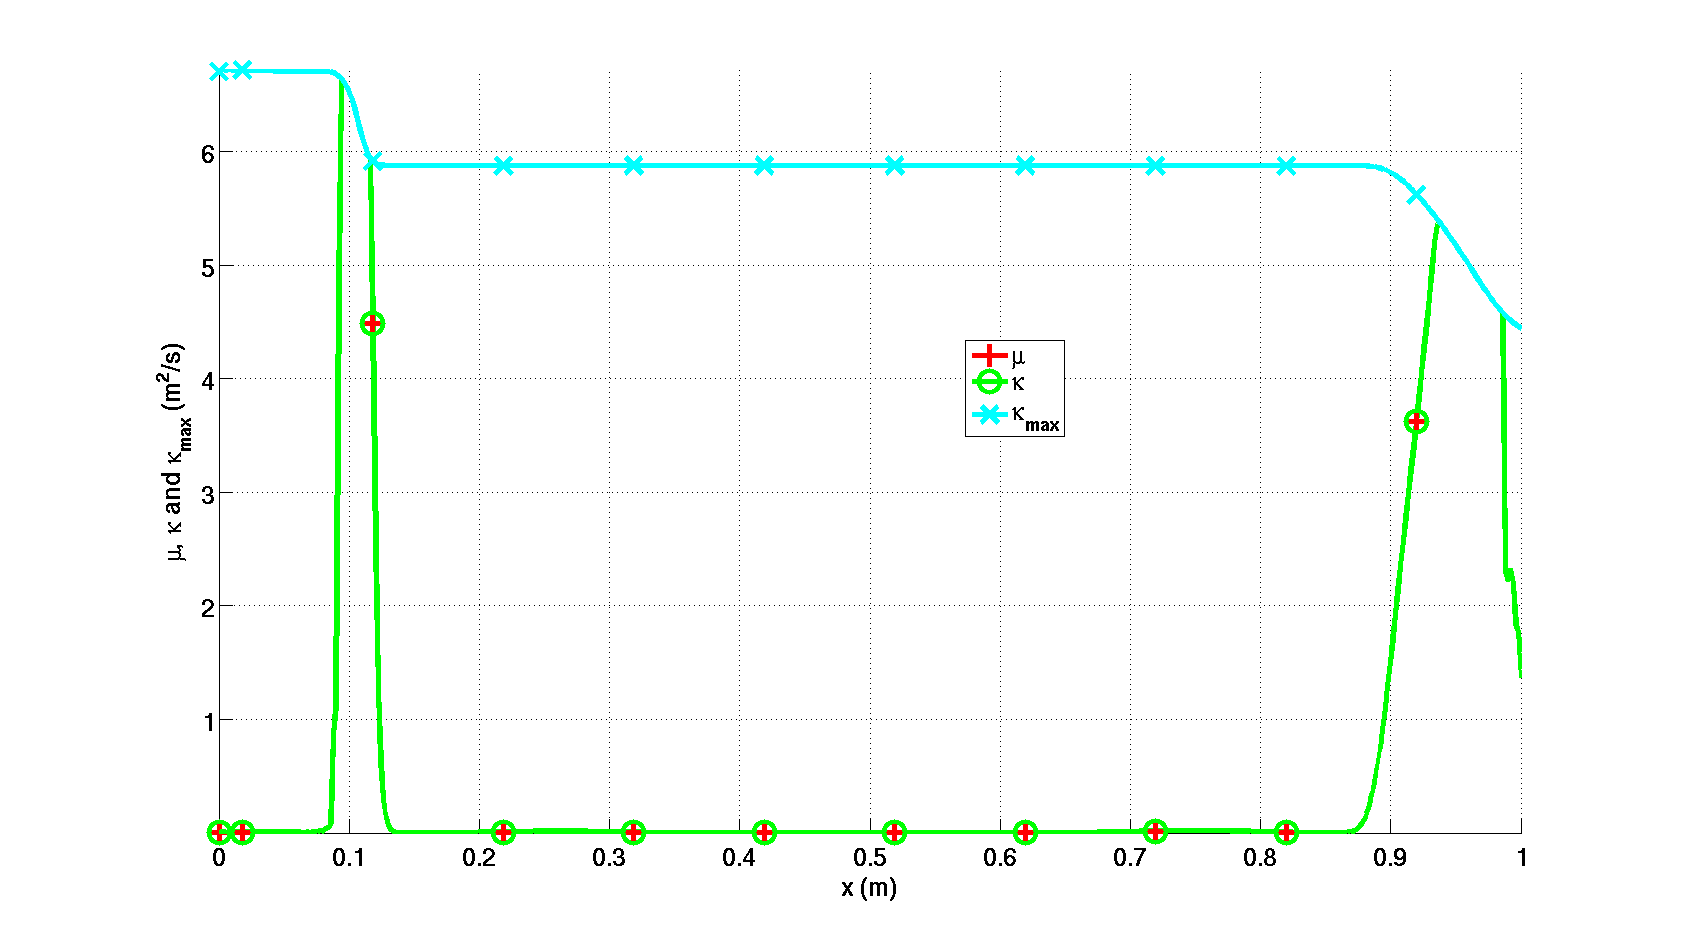
\includegraphics[width=\textwidth]{figures/Plot_viscosity_gas_phase.png}
%                \caption{Gas viscosity coefficients}
%                \label{fig:vap-phase-visc}
%        \end{subfigure}
%        \caption{Numerical solutions for the vapor phase of a two-phase water hammer at times $t=8.7 \times 10^{-4}, \, 6.8 \times 10^{-3} \text{ and } 10^{-3}$ s (the viscosity coefficients are only shown at time $t=8.7 \times 10^{-4}$ s).}\label{fig:vapor-phase}
%\end{figure}
%%
%\fig{fig:liquid-phase} and ~\ref{fig:vapor-phase} show that the numerical solution of the liquid and gas phases do not display any oscillations or instabilities. 
%As expected, the two fluids have the same pressure and velocity profiles as shown in \fig{fig:vap-phase-press}, ~\ref{fig:liq-phase-press} and \fig{fig:vap-phase-vel}, ~\ref{fig:liq-phase-vel}, respectively. The waves  coming from the left and right walls are initially well resolved and do not display any instability but lose sharpness over time for the same reason as detailed in \sct{sec:single-num-res}. The density of the liquid and gas phases have different values but experience similar variations. The viscosity coefficients are plotted at time $t = 8.7 \times 10^{-3}$ s and display two peaks that match the shock positions.
%
%%%%%%%%%%%%%%%%%%%%%%%%%%%%%%%%%%%%%%%%%%%%%%%%%%%%%%%%%%%%%%%%%%%%%%%%%%%%%
%%%%%%%%%%%%%%%%%%%%%%%%%%%%%%%%%%%%%%%%%%%%%%%%%%%%%%%%%%%%%%%%%%%%%%%%%%%%%
\section{Conclusions and future work}\label{sec:conclusion}
%%%%%%%%%%%%%%%%%%%%%%%%%%%%%%%%%%%%%%%%%%%%%%%%%%%%%%%%%%%%%%%%%%%%%%%%%%%%%
%%%%%%%%%%%%%%%%%%%%%%%%%%%%%%%%%%%%%%%%%%%%%%%%%%%%%%%%%%%%%%%%%%%%%%%%%%%%%
%
In this paper, we have presented two sets of results involving single- and two-phase flows developing pressure waves simulated with the RELAP-7 system code. The EVM was used to stabilize the numerical solution.

Three single-phase shock tubes tests were simulated with air, liquid water and vapor using ideal and real equations of state, and showed that the EVM can accurately resolved the shock, contact, and rarefaction waves. Single-phase numerical results compared well against solutions obtained with the RELAP-5 and WAHA system codes from \cite{Sokolowski-Koszela}. A two-phase flow shock tube taken from the published literature was also performed with RELAP-7 in the case where the seven-equation model devolves to the HEM. Using the EVM as a stabilization technique, we observe that the numerical solutions compare well against results obtained with the RELAP-5 and WAHA system codes. For both set of tests, a mesh sensitivity analysis is also performed and shows that the accuracy of the numerical solution is improved when refining the mesh. 

Overall, these tests demonstrate the capabilities of the EVM to resolved single- and two-phase shock tubes in the RELAP-7 code when using steam-water tables. Ongoing and future work will include the simulation of waterhammer tests; such tests require the implementation of appropriate mass and heat transfer correlations, and thus will be the focus of a future communication.
%We have presented numerical results of single- and a two-phase water hammers obtained with the system code RELAP-7. The numerical results show that the Entropy Viscosity Method is capable of stabilizing the schemes and that the viscosity coefficients are well-scaled. This work contributes to the assessment of the stabilization techniques for reactor flow problems computed with RELAP-7.

%%%%%%%%%%%%%%%%%%%%%%%%%%%%%%%%%%%%%%%%%%%%%%%%%%%%%%%%%%%%%%%%%%%%%
\section{Acknowledgments}

This research was carried out under the auspices of the Idaho National Laboratory, a contractor of the U.S. Government under contract No. DEAC07-05ID14517.  Accordingly, the U.S. Government retains a non-exclusive, royalty-free license to publish or reproduce the published form of this contribution, or allow others to do so, for U.S. Government purposes.
%\tcr{copy the Acknowledgments of our 7eq paper. It has all of the information that INL wants to see here. Ray will have to tell us if the DOE contract number for INL's management must be updated} \tcb{done}

%%%%%%%%%%%%%%%%%%%%%%%%%%%%%%%%%%%%%%%%%%%%%%%%%%%%%%%%%%%%%%%%%%%%%
\setlength{\baselineskip}{12pt}

\bibliographystyle{inputs/mc2015}
\bibliography{mybibfile}



\end{document}
